\chapter{Results}
In this section, results from the computation using the implemented software are presented. There are two classical benchmarks for 3-dimensional MHD equations, namely the MHD Blast \cite{blast1}, \cite{blast2}, and the Orszag-Tang vortex \cite{vortex}. And then the main section of this work contains results from the flux tube eruption model on and above the Sun's surface.
\paragraph{}
In most cases, we are interested in the distribution of plasma density $\rho$ and the magnetic field $B$ in the domain $\Omega$.

\section{Benchmarks}
\label{sec:benchmarks}
The benchmarks presented in this Section do not have an exact analytical solution, but the formation of waves and discontinuities is well studied, and benchmarking is usually performed on the basis of comparing the structure and presence of non-physical attributes.
\subsection{Hardware specification}
For all following benchmarks, the setup described below was used. The computational mesh $T_h$ was formed in all cases by rectangular hexahedra.
The value of the time step $\tau$ used was set according to the CFL condition (\cref{section:CFL}).
The Taylor basis functions (see \cite{KuzminVertex}) and Divergence-free basis functions (\cref{tbl:divFreeBasis}) of order $0$ (piecewise constant functions) and $1$ (piecewise linear functions) were used.
Where appropriate (for piecewise linear basis functions), the slope limiting technique from \cref{sec:vertex} was used.
Illustration of the obtained results follows below - these results were obtained using one node of the department's computational cluster with these parameters:
\begin{itemize}
    \item CPU: Intel(R) Xeon(R) CPU E5-2680 v3 @ 2.50GHz,
    \item \# of Cores: 48 per node (nodes 1, 2), 16 per node (nodes 3, 4),
    \item Vectorization support: AVX2,
    \item Parallelization implemented: Intel TBB,
    \item Distributed calculation implemented: OpenMPI,
    \item RAM: 512 GB,
    \item C/C++ Compiler: GNU gcc 5.4.0 .
\end{itemize}

\subsection{MHD Blast}
\subsubsection{MHD Blast - original version}
This benchmark has been used for decades - \cite{blast0}, \cite{blast1}, \cite{blast2} - in a variety of configurations and as a benchmark in software - e.g. \citep{athena}. The setup as described in \cite{blast0}, \cite{blast1} is defined (although in \cite{blast1} with interchanged $x-$ and $y-$ coordinates) by the initial conditions:
\begin{align}
\label{mhdBlastOld}
\gamma & =  5 / 3\\ \nonumber
p_0\lo\bfx, t\ro & =  100\ \ \text{for}\ \left|\bfx\right| < 0.1\\ \nonumber
p_0\lo\bfx, t\ro & =  1\ \ \text{for}\ \left|\bfx\right| \geq 0.1\\ \nonumber
\rho\lo\bfx, t = 0\ro & =  1,\\ \nonumber
p\lo\bfx, t = 0\ro & =  p_0\lo\bfx, t\ro,\\ \nonumber
\bfu_1\lo\bfx, t = 0\ro & =  0,\\ \nonumber
\bfu_2\lo\bfx, t = 0\ro & =  0,\\ \nonumber
\bfu_3\lo\bfx, t = 0\ro & =  0,\\ \nonumber
\bfB_1\lo\bfx, t = 0\ro & =  0,\\ \nonumber
\bfB_2\lo\bfx, t = 0\ro & =  100,\\ \nonumber
\bfB_3\lo\bfx, t = 0\ro & =  0.
\end{align}
Total energy is calculated using \cref{magU,kinU,presU}.
The domain $\Omega$ is a square, with scaling quite arbitrarily used in the papers. In the case of \cite{blast1}, $\Omega = [0, 1] \times [0, 1]$, in this work it is $\Omega = [-0.25, 0.25] \times [-0.25, 0.25]$.

It is obvious from the initial setup, that the example is true to its name, and it is in fact a blast of the over-pressured area $\left|\bfx\right| < 0.1$, where pressure $p$ is 100$\times$ larger than elsewhere in the domain. This setup is completed with simple outflow boundary condition \cref{bcoutdef}.
In the next figures, the solution as presented in \cite{blast1} is compared to the solution obtained with the approach described in this work. Note that the solution from \cite{blast1} needed to have the axes transformed $\lo x\rightleftharpoons y\ro$ with respect to the original paper. The figure \cref{figure:blastOldRef} is taken from the article \cite{blast1} from the page 33. Unfortunately the paper does not specify the precise time at which the snapshots are taken.

\begin{figure}[H]
\centering
\hspace{-8mm}
\begin{subfigure}[b]{0.4\textwidth}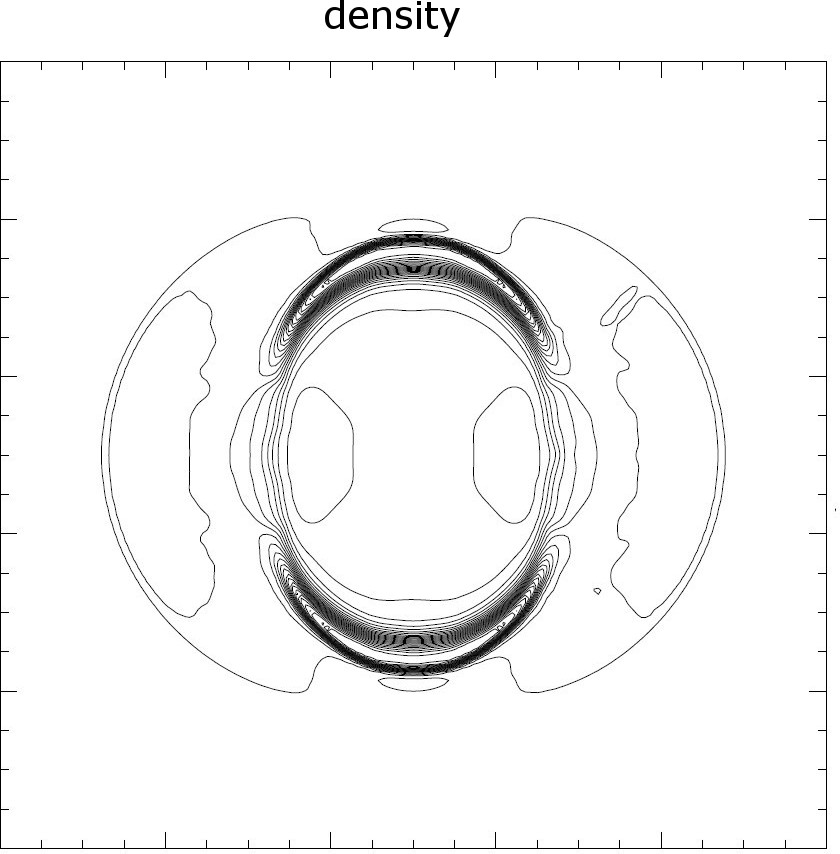
\includegraphics[width=\textwidth]{img/mhd-blast/old/ref.jpg}\end{subfigure}
\begin{subfigure}[b]{0.395\textwidth}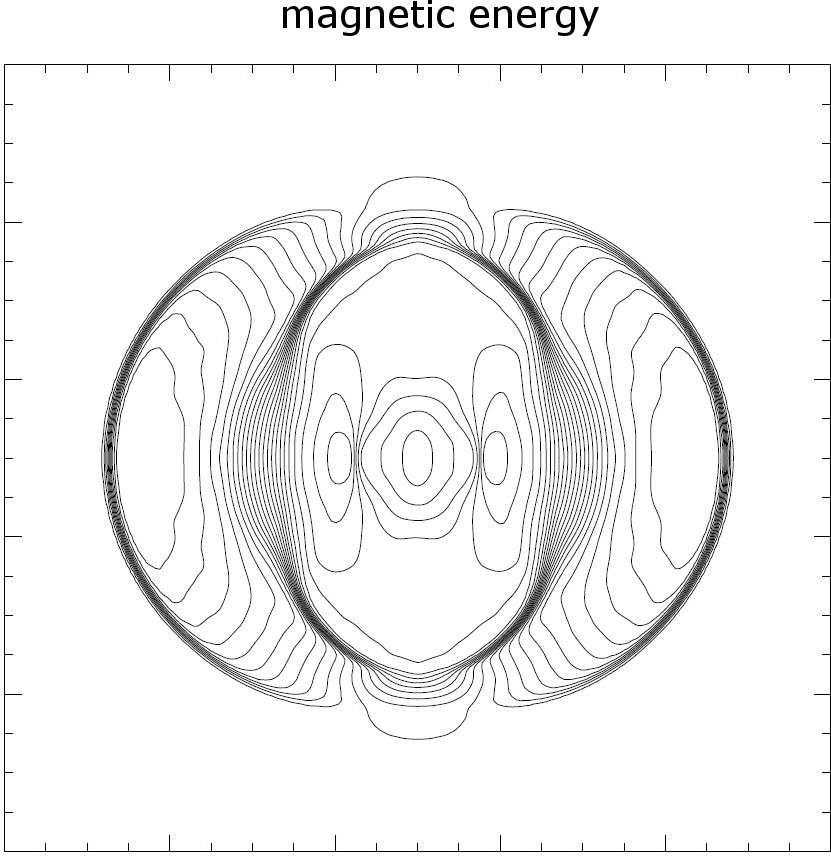
\includegraphics[width=\textwidth]{img/mhd-blast/old/refmag.jpg}\end{subfigure}
\caption{Results from \cite{blast1}, density(left), magnetic energy(right)}
\label{figure:blastOldRef}
\end{figure}

\vspace{-5mm}
\begin{figure}[H]
	\begin{center}
		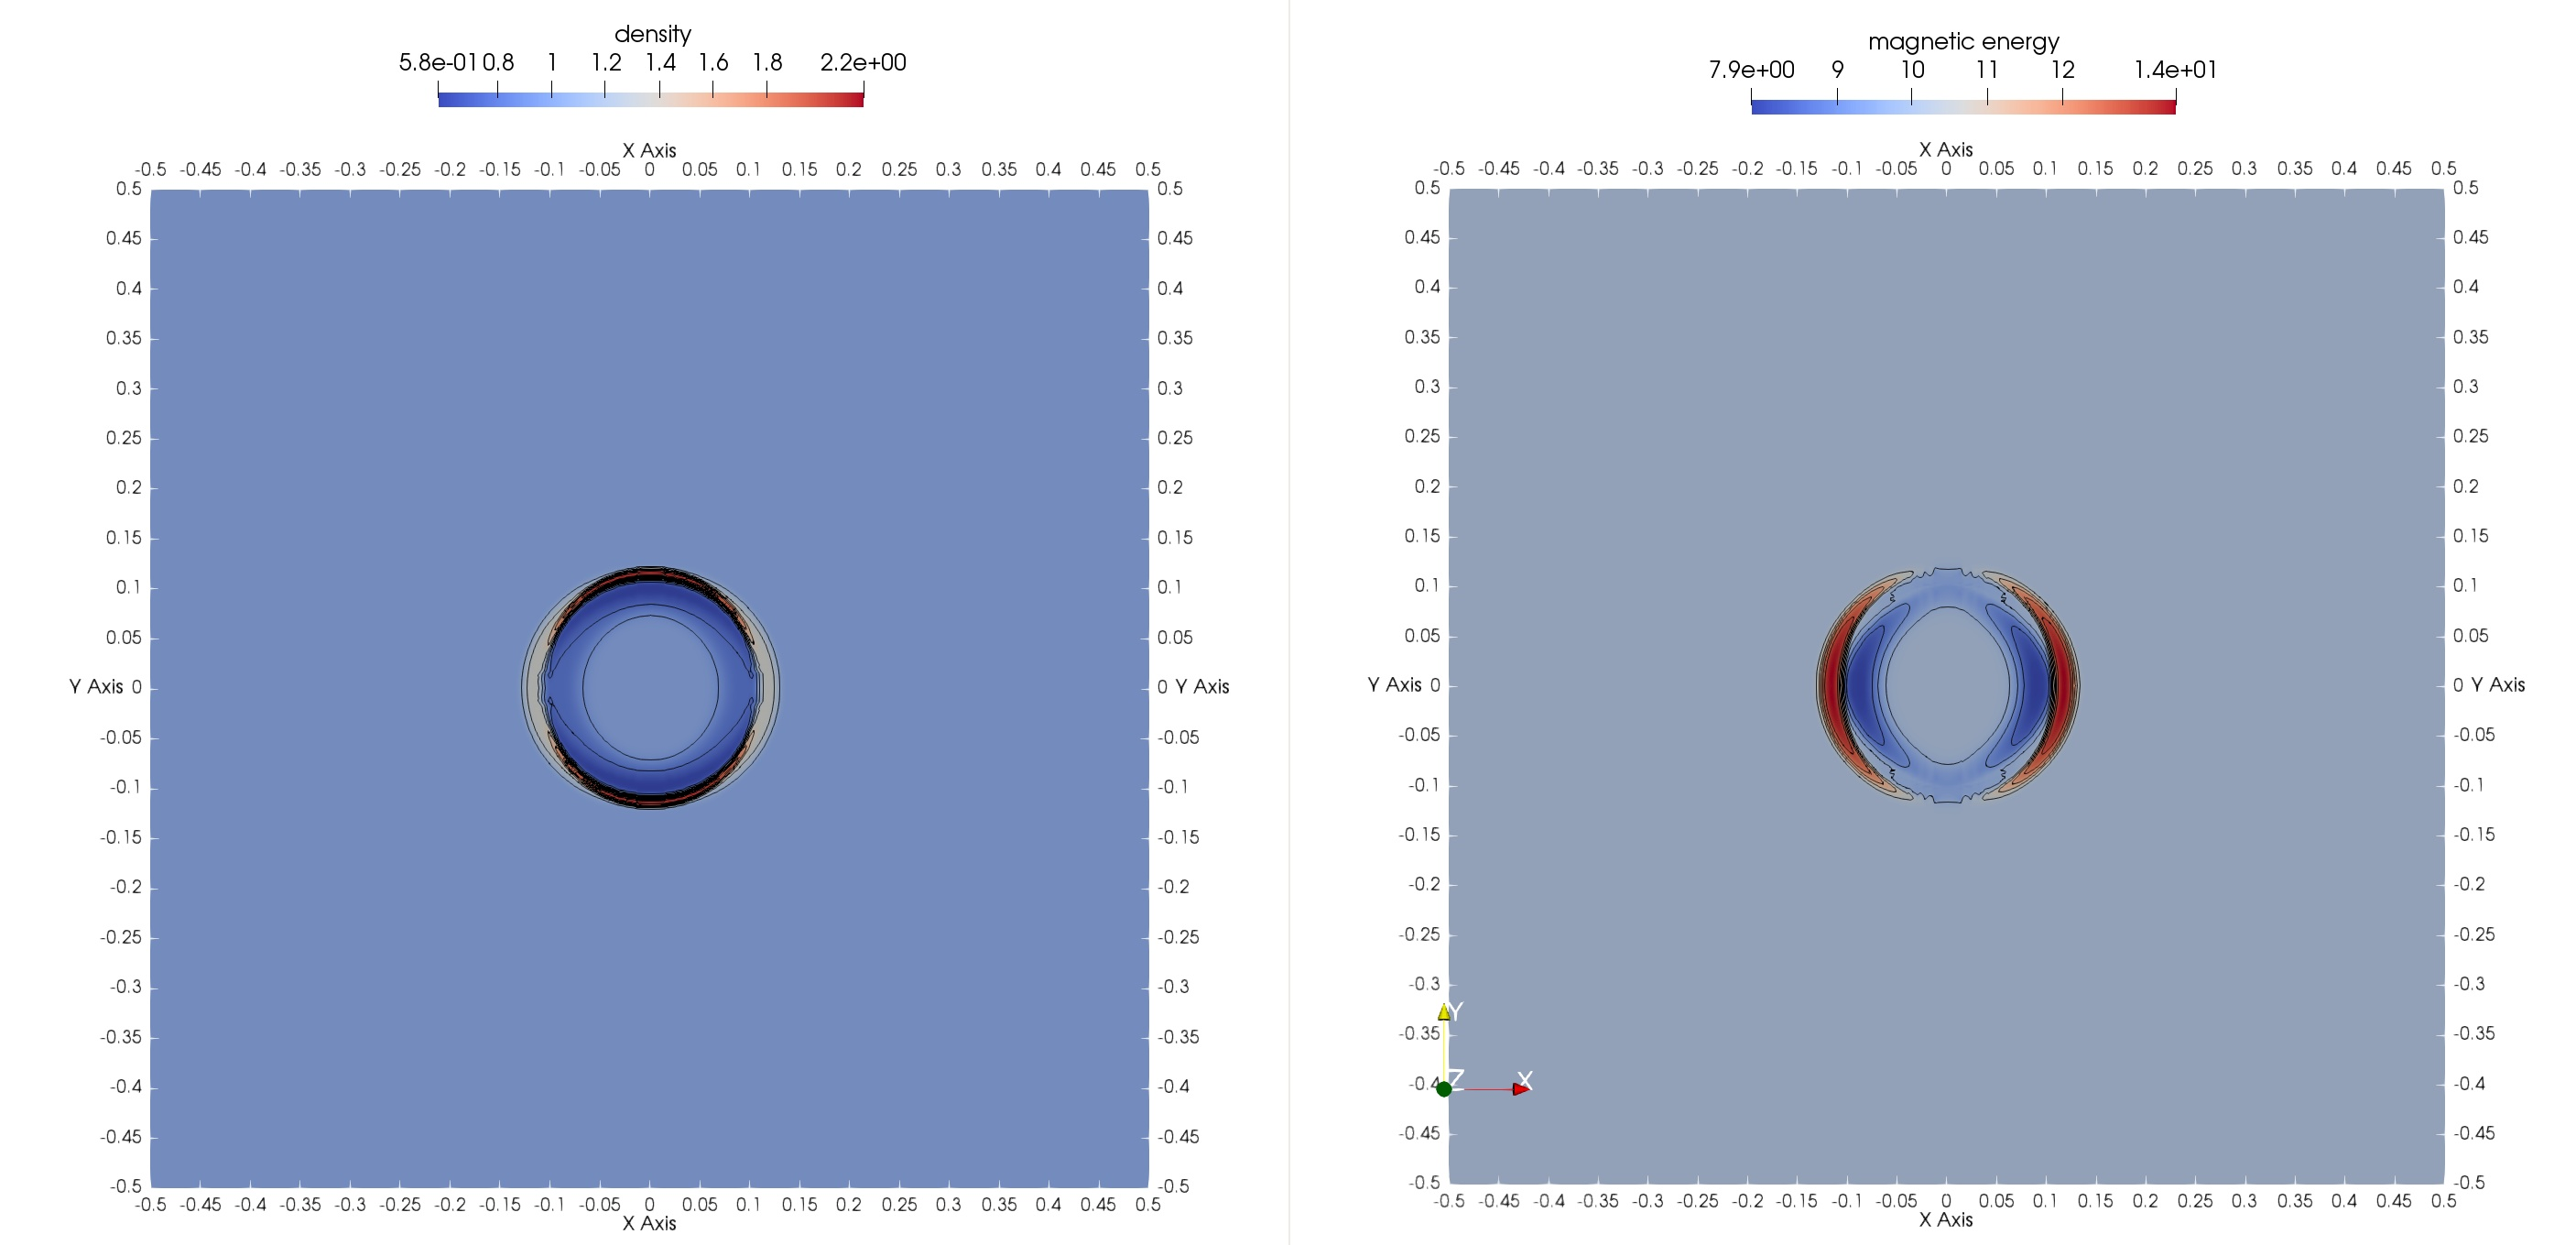
\includegraphics[width=0.87\textwidth]{img/mhd-blast/old/mynew1.jpg}
	\caption{Obtained results, $t = 1\times 10^{-3}$, density(left), magnetic energy(right)}
	\label{figure:blastOldMy1}
	\end{center}
\end{figure}
\vspace{-8mm}

\begin{figure}[H]
	\begin{center}
		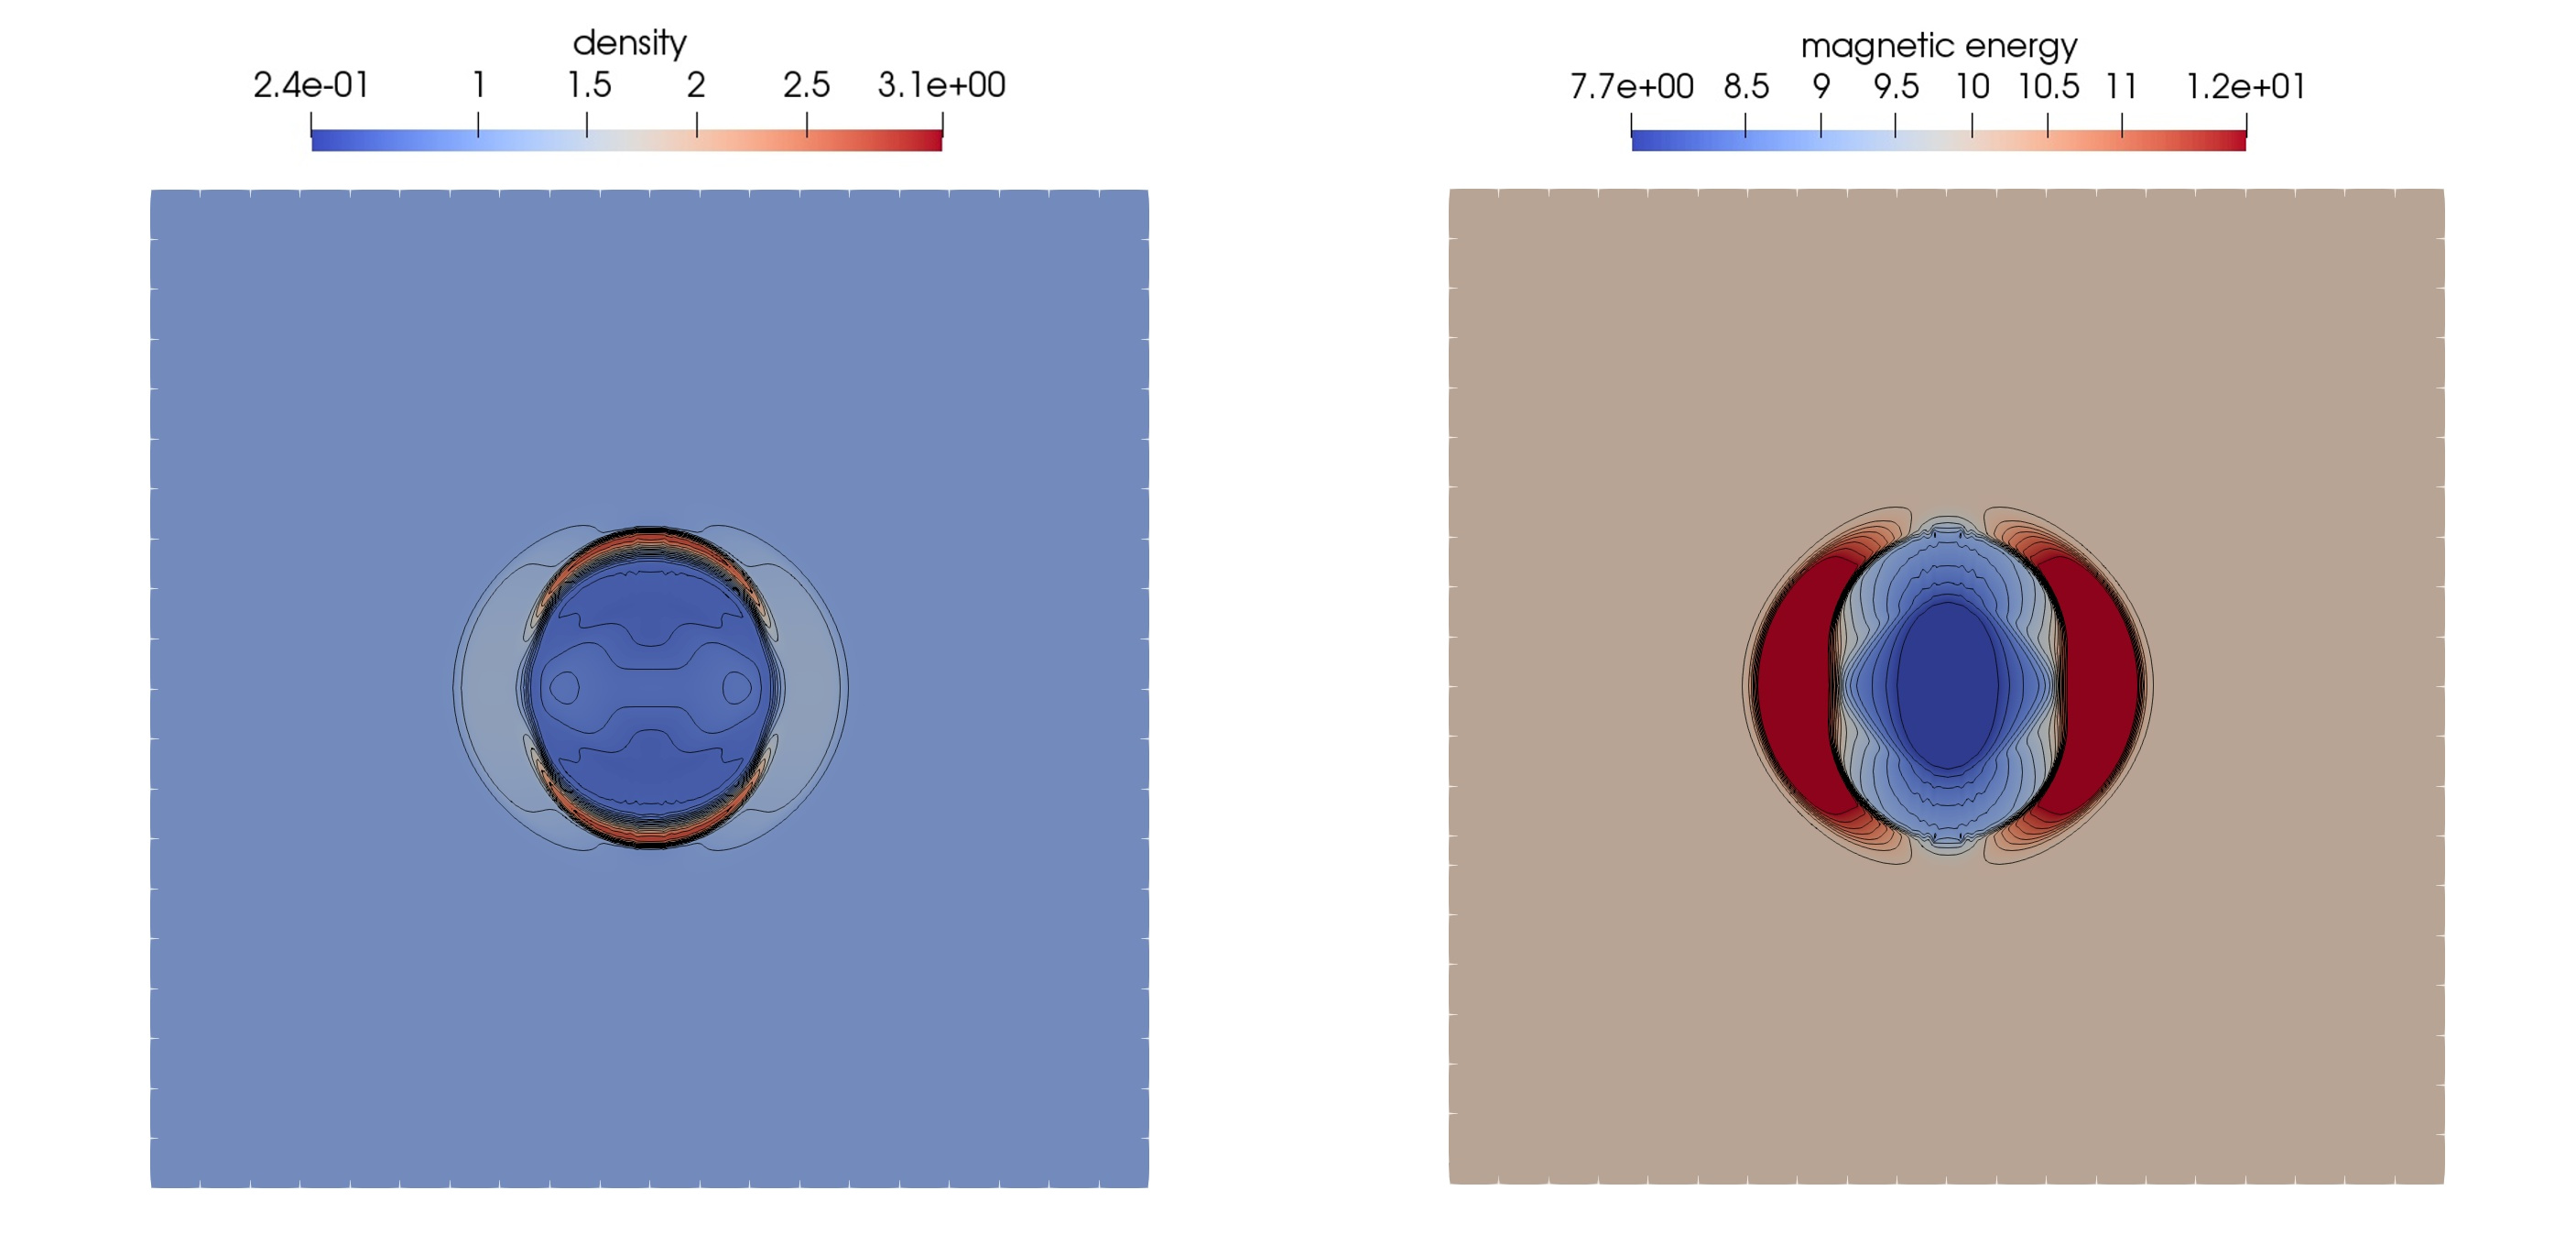
\includegraphics[width=0.87\textwidth]{img/mhd-blast/old/mynew2.jpg}
	\caption{Obtained results, $t = 6\times 10^{-3}$, density(left), magnetic energy(right)}
	\label{figure:blastOldMy2}
	\end{center}
\end{figure}
\vspace{-8mm}

\begin{figure}[H]
	\begin{center}
		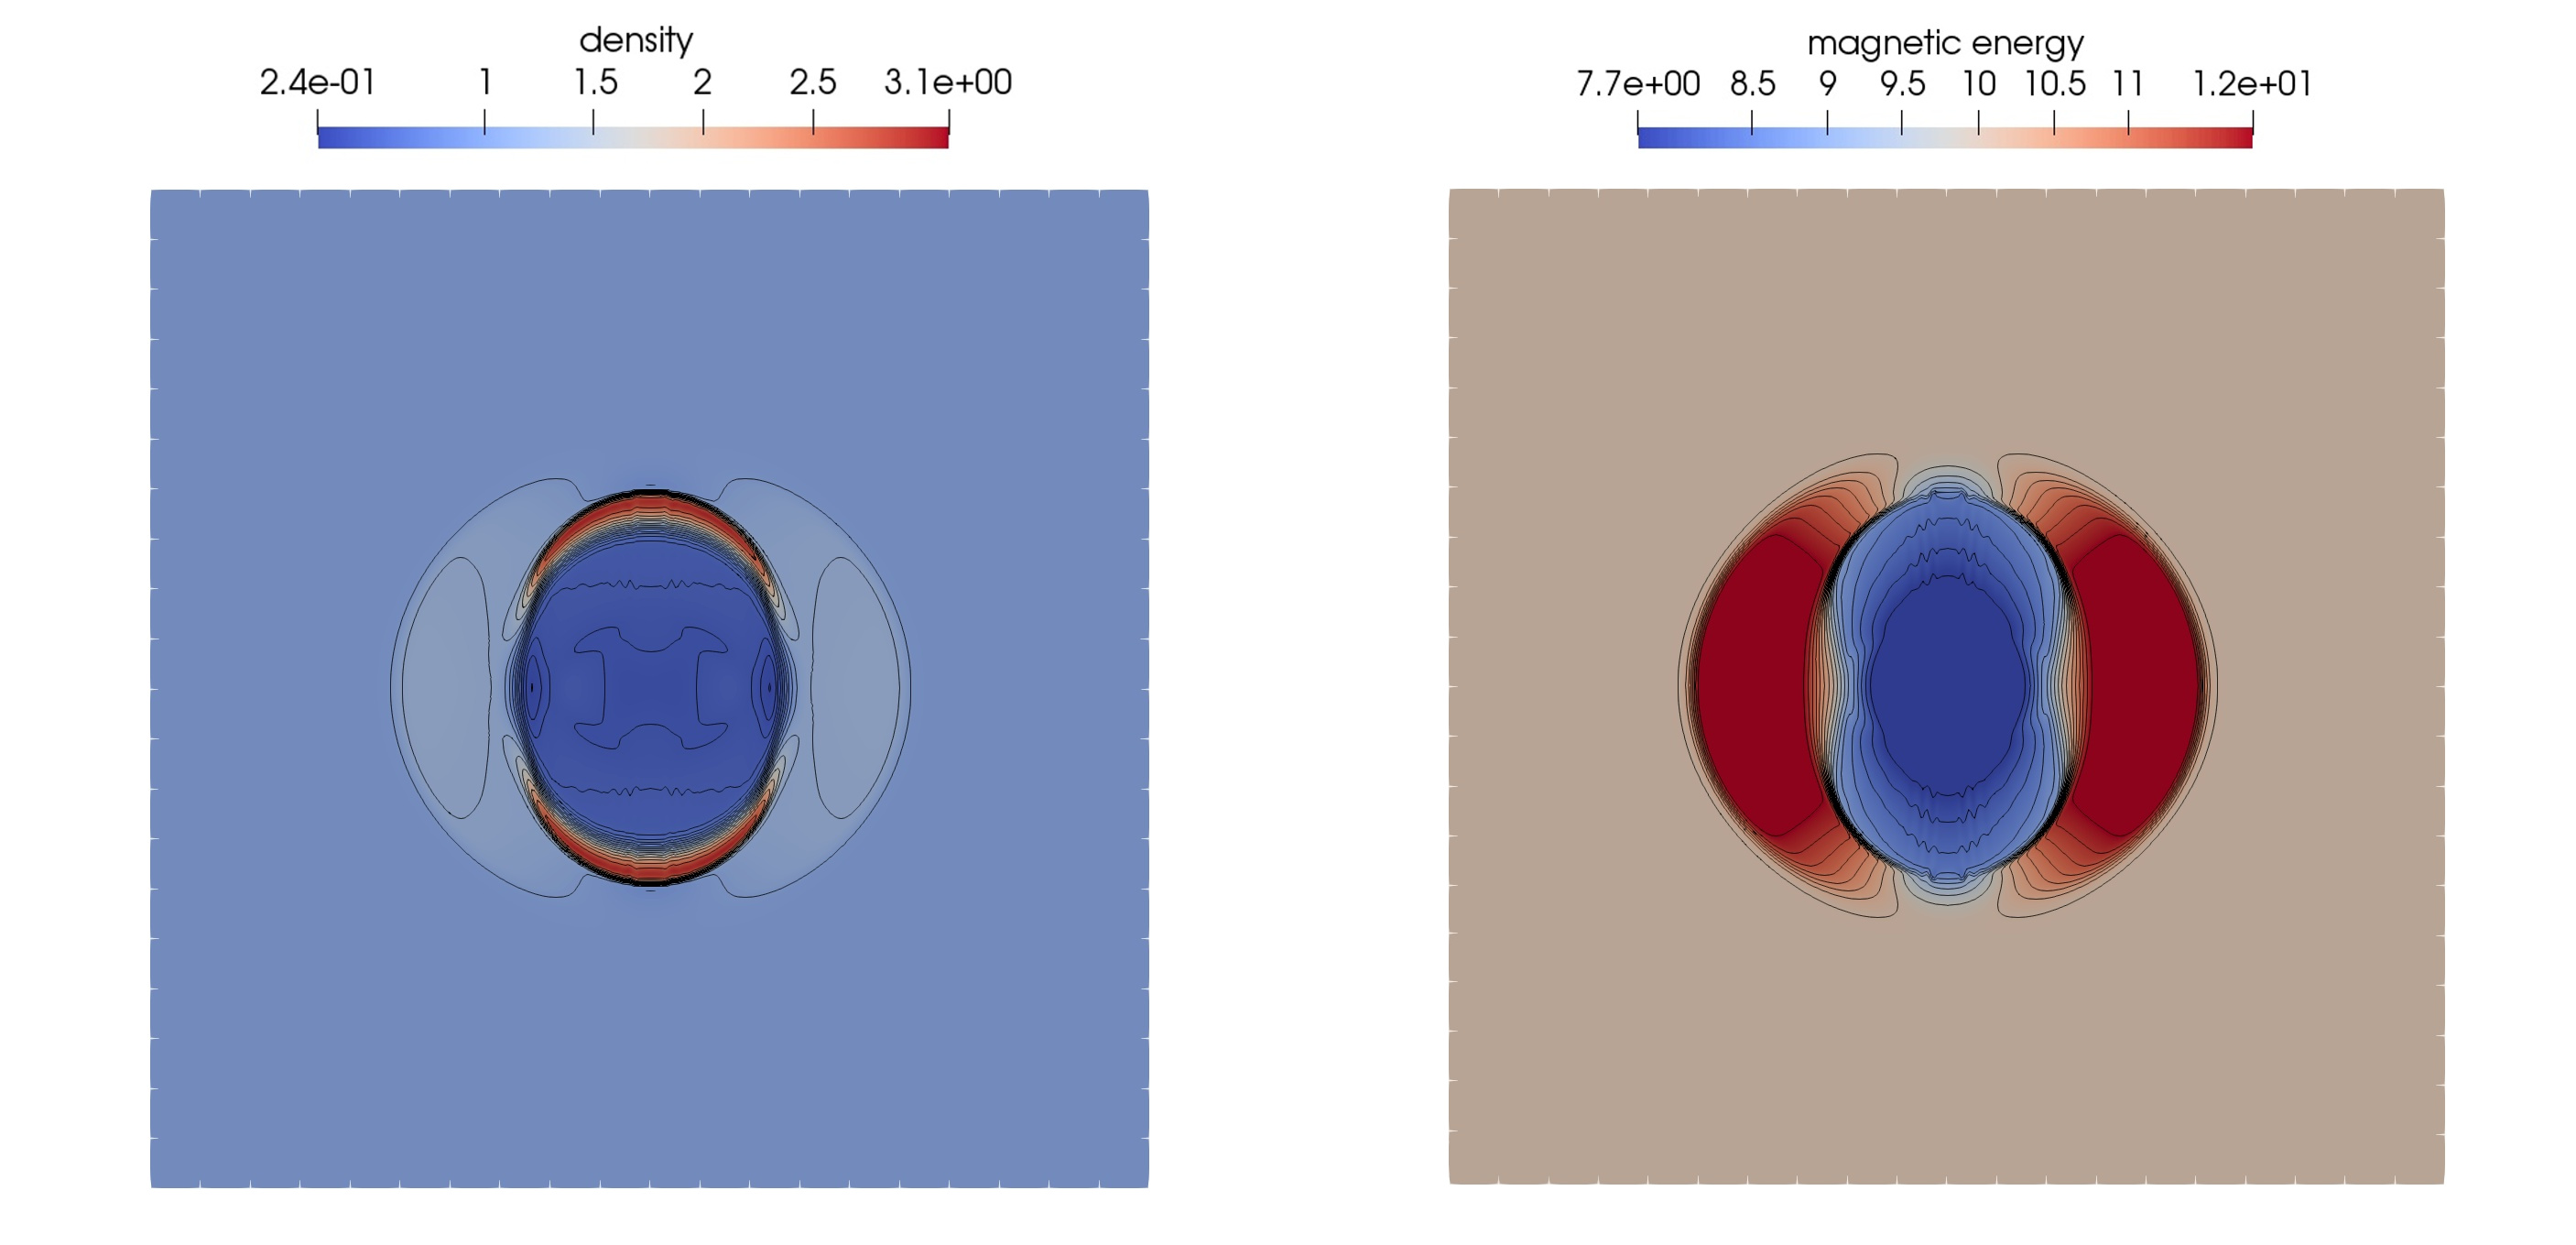
\includegraphics[width=0.87\textwidth]{img/mhd-blast/old/mynew3.jpg}
	\caption{Obtained results, $t = 11\times 10^{-3}$, density(left), magnetic energy(right)}
	\label{figure:blastOldMy3}
	\end{center}
\end{figure}
\vspace{-8mm}

\begin{figure}[H]
	\begin{center}
		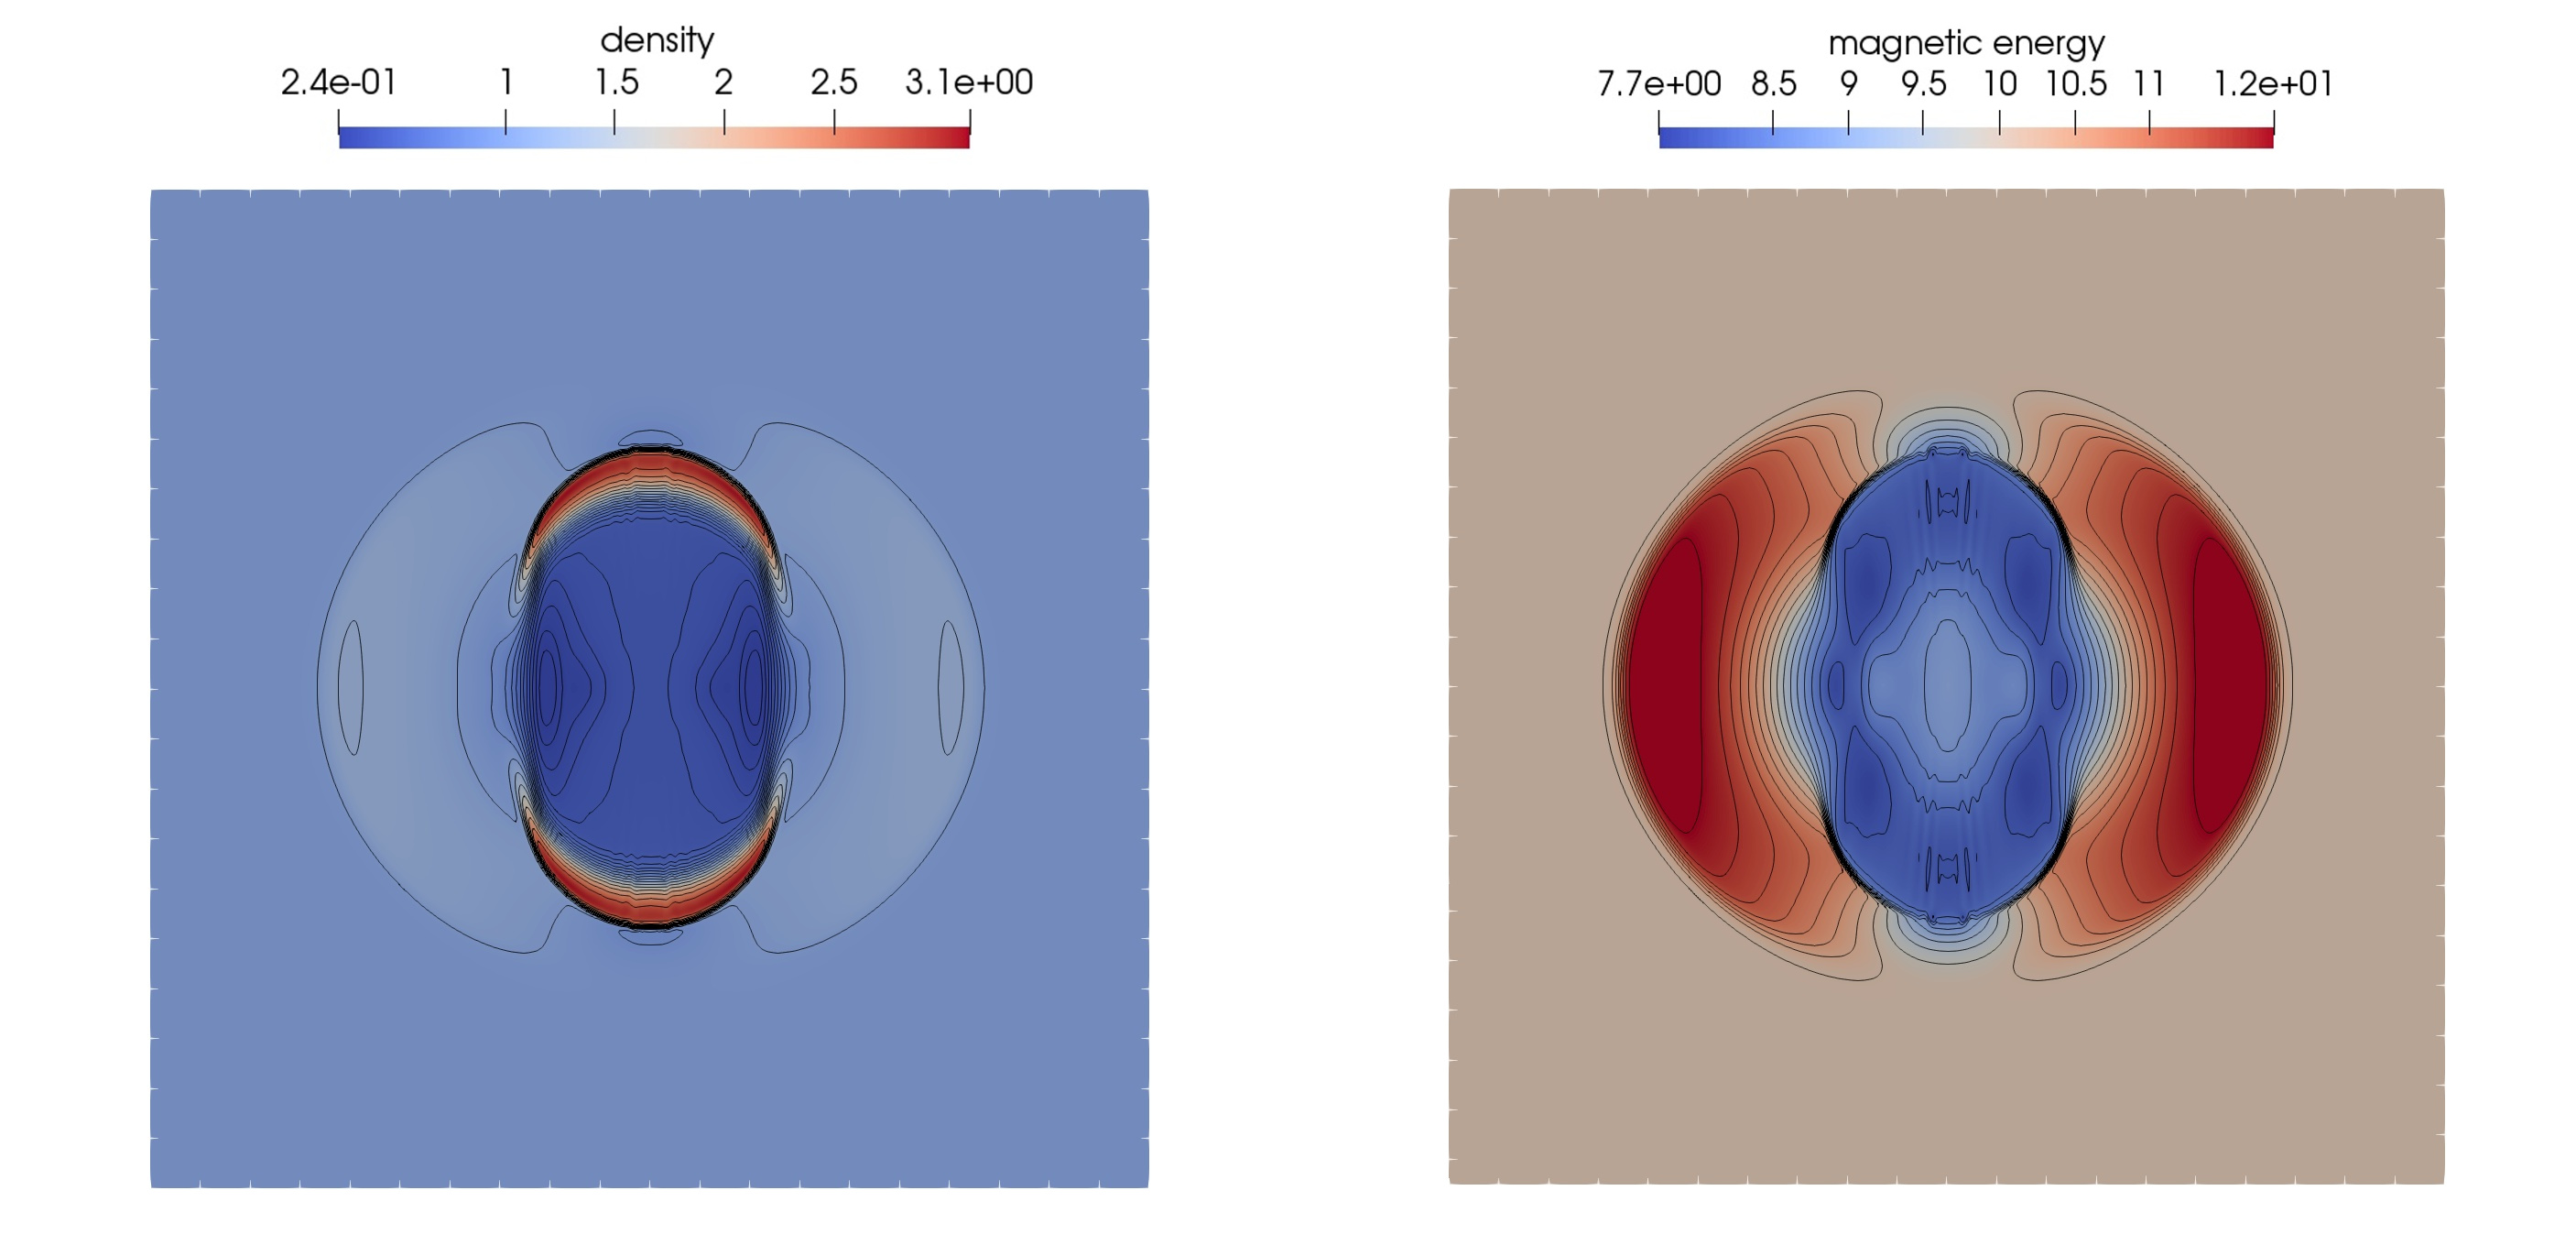
\includegraphics[width=0.87\textwidth]{img/mhd-blast/old/mynew4.jpg}
	\caption{Obtained results, $t = 16\times 10^{-3}$, density(left), magnetic energy(right)}
	\label{figure:blastOldMy4}
	\end{center}
\end{figure}
\vspace{-8mm}

\begin{figure}[H]
	\begin{center}
		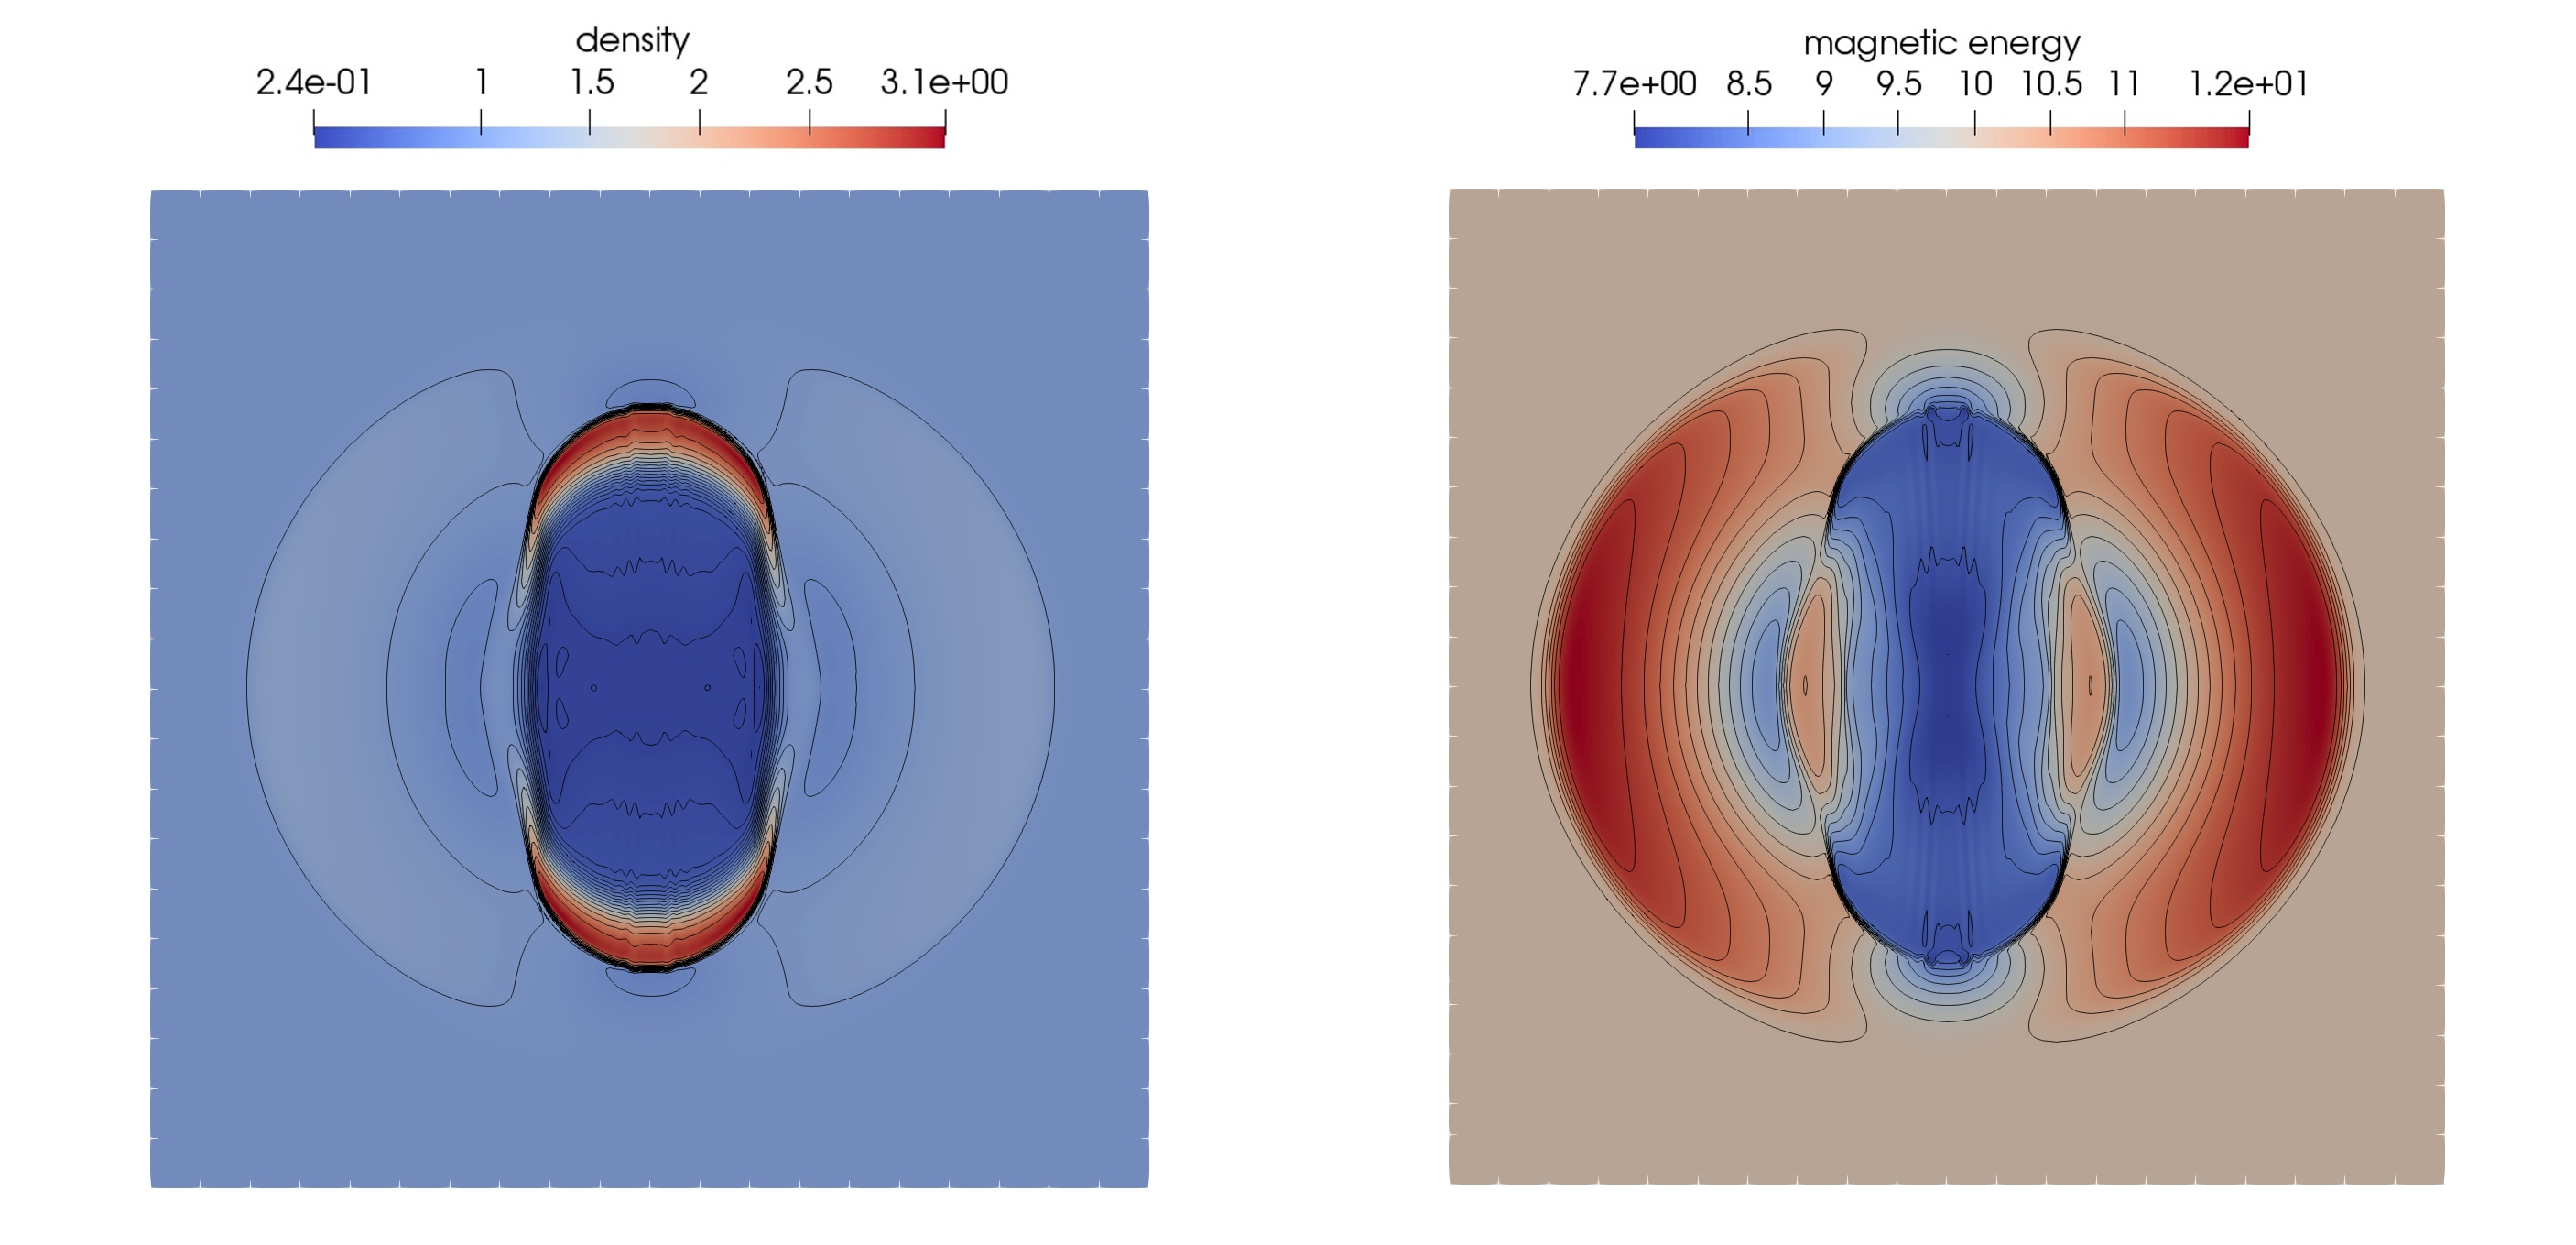
\includegraphics[width=0.87\textwidth]{img/mhd-blast/old/mynew5.jpg}
	\caption{Obtained results, $t = 23\times 10^{-3}$, density(left), magnetic energy(right)}
	\label{figure:blastOldMy5}
	\end{center}
\end{figure}
\vspace{-5mm}
The solution in \cref{figure:blastOldMy4,figure:blastOldMy5}  is apparently almost identical to that in \cref{figure:blastOldRef}. To demonstrate the distributed nature of the computation, in \cref{figure:subdomainsBlastOld}, color-mapping of elements $K \in T$ to processors owning the particular element is presented (see \cref{section:ditributedTria} for details). Note that there were $48$ processors used for the computation.

\begin{figure}[H]
	\begin{center}
		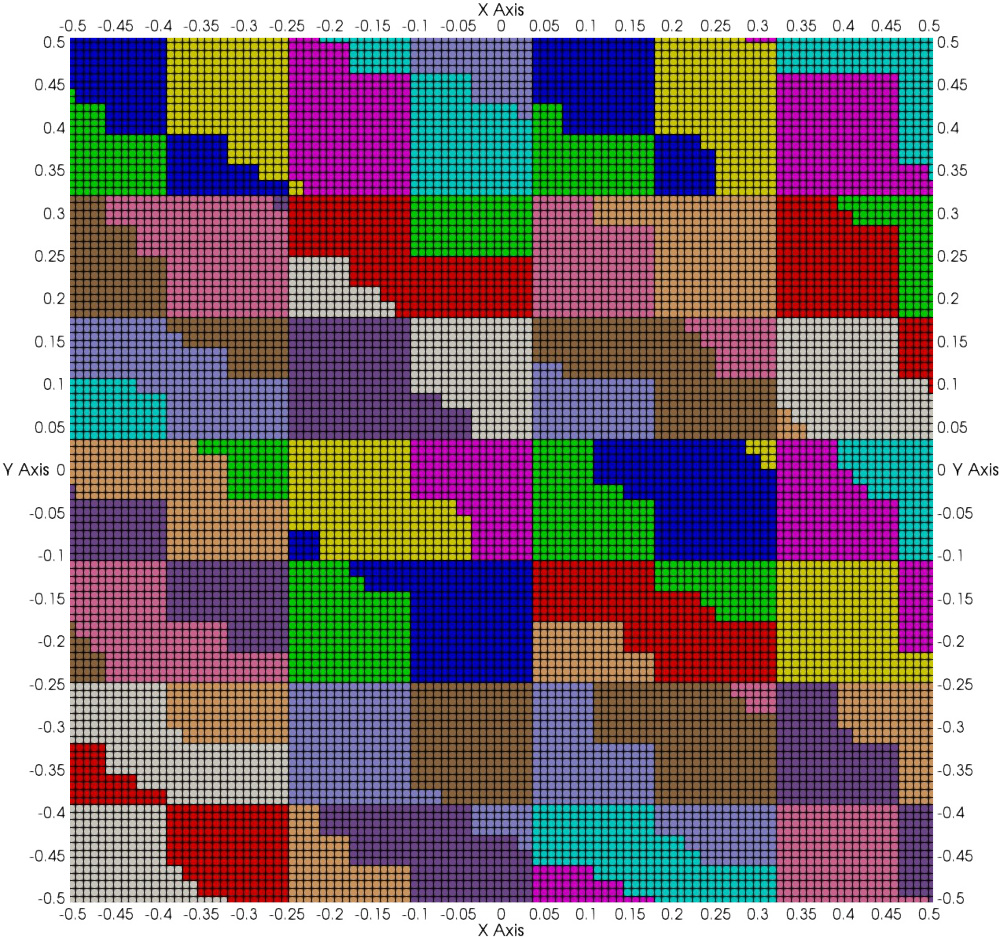
\includegraphics[width=0.65\textwidth]{img/mhd-blast/old/subdomain.jpg}
	\caption{Color-mapping of elements to processors for the computation of \crefrange{figure:blastOldMy1}{figure:blastOldMy5}}
	\label{figure:subdomainsBlastOld}
	\end{center}
\end{figure}
\vspace{-5mm}

This however, was a static calculation with 200 mesh elements in the $x-$ and $y-$ dimensions. In order to see how the AMR (see \cref{chapter:amr}) performs, the same computation was performed in adaptive setup. Starting from a very coarse mesh of 10 elements in both dimensions, the evolving mesh and its distribution to processors are shown in \crefrange{figure:blastOldMyAdapt1}{figure:blastOldMyAdapt6} - the distribution to processors on the left, the mesh elements on the right.

\begin{figure}[H]
	\begin{center}
		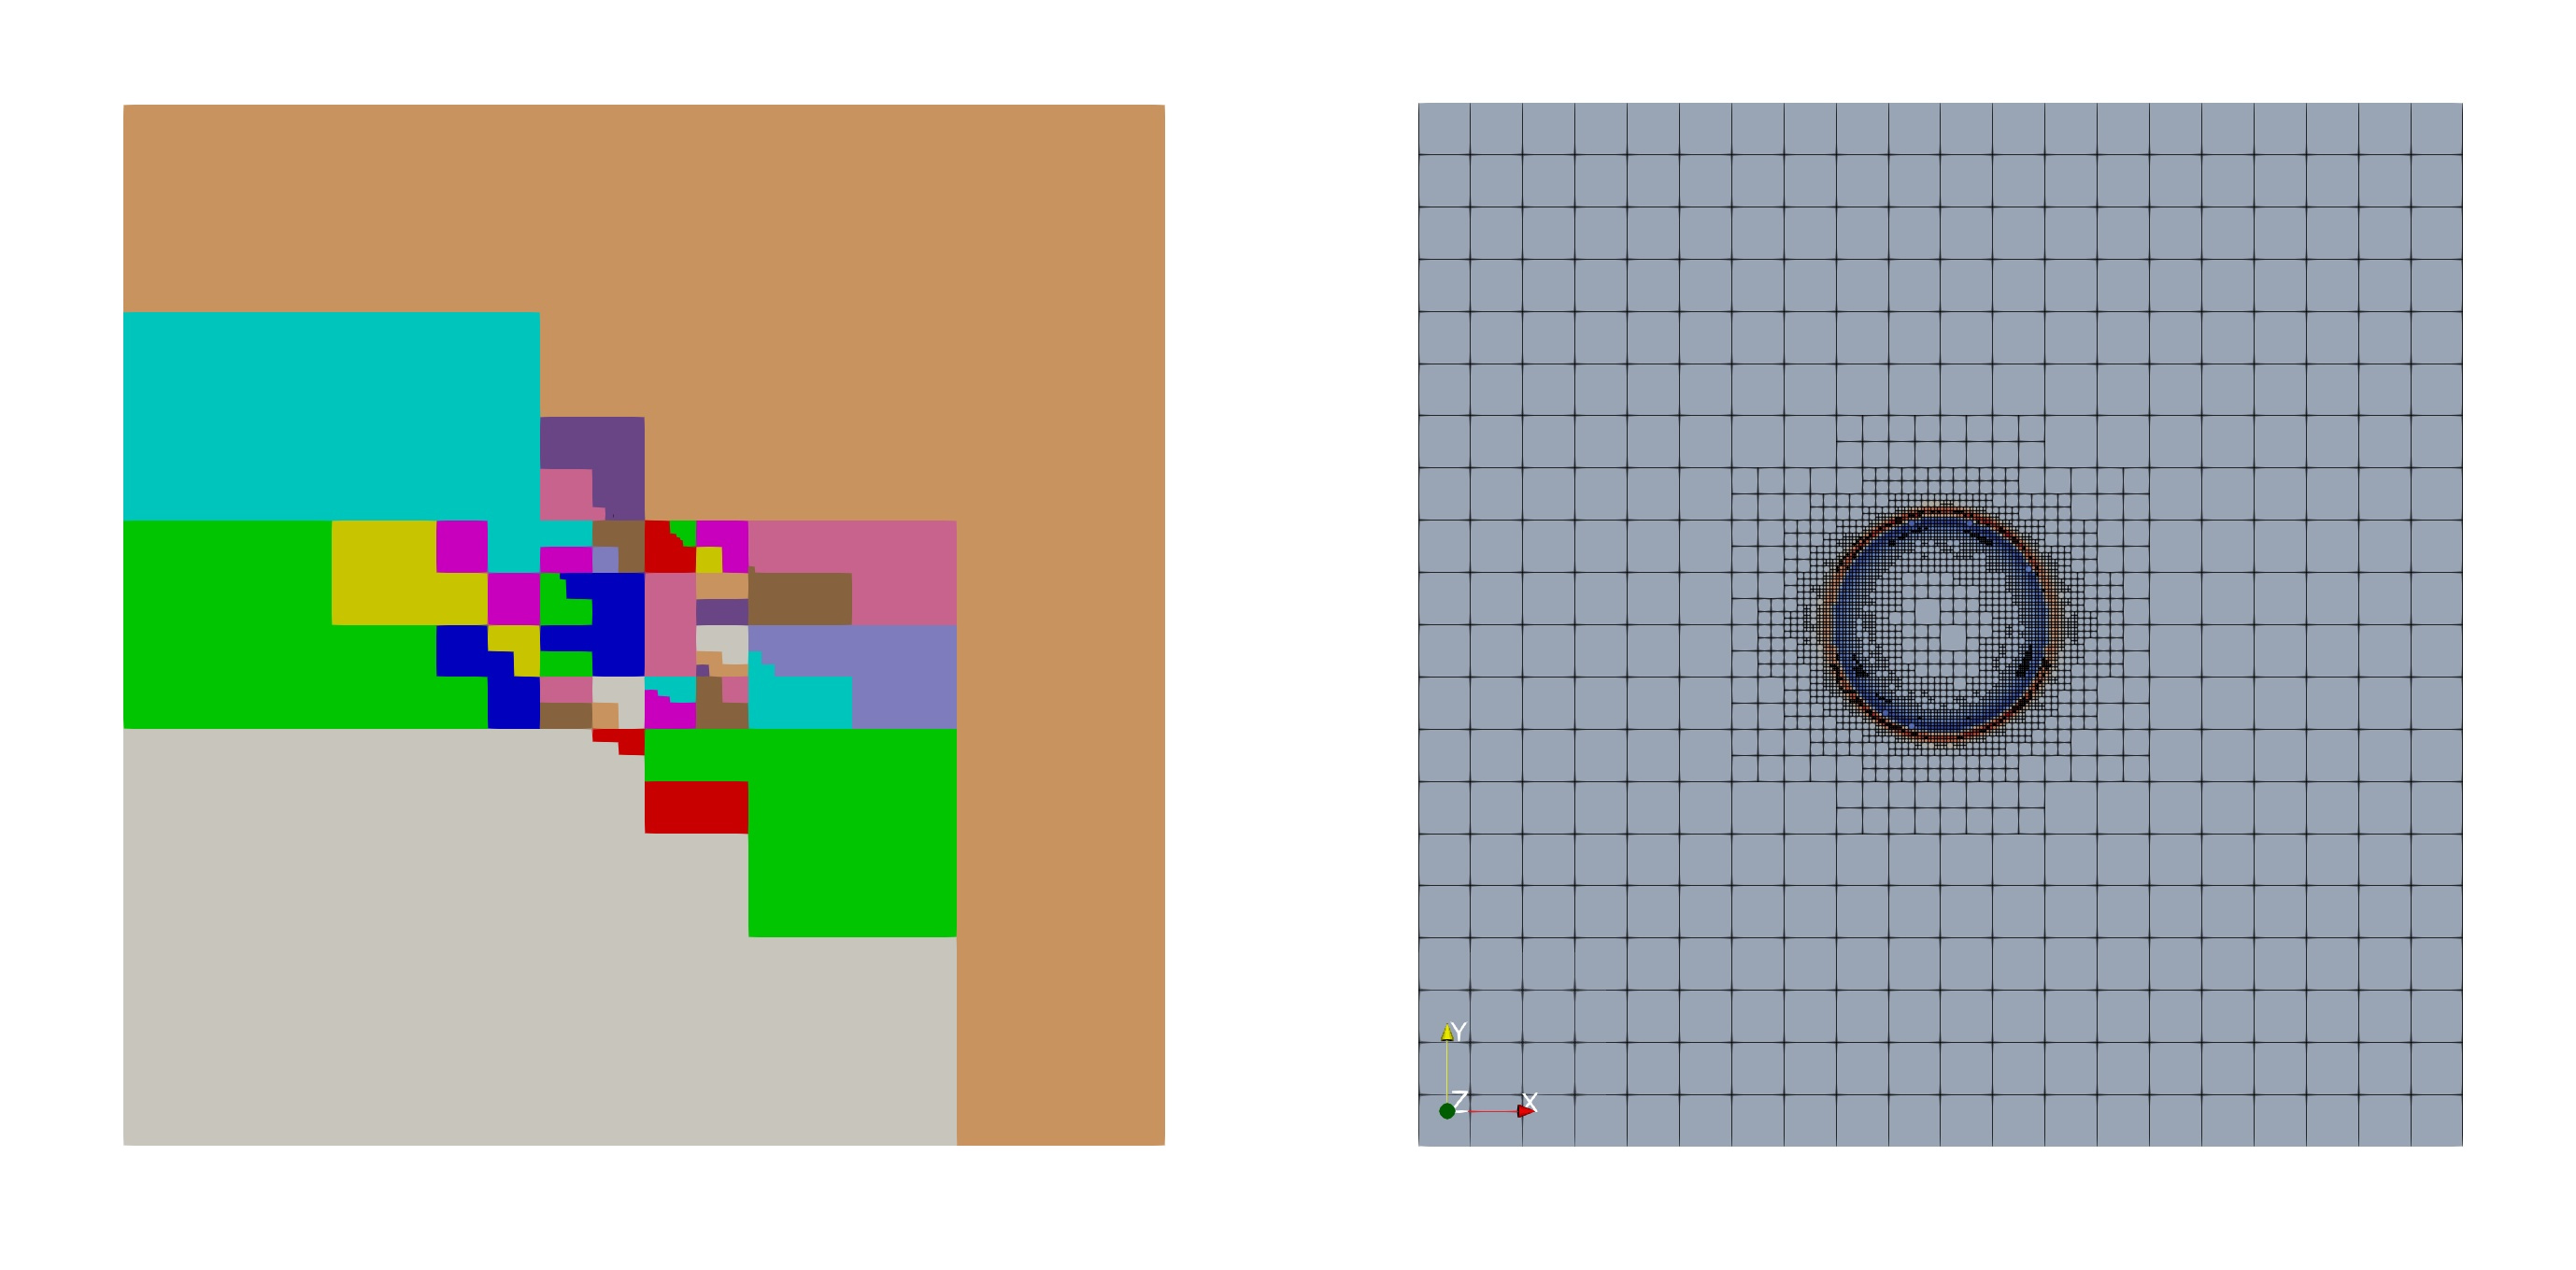
\includegraphics[width=0.87\textwidth]{img/mhd-blast/old/mya1.jpg}
	\caption{Obtained results, initial state, distribution of $\rho$ on elements in $T\lo\Omega\ro$ (right) and distribution of these elements to processors (left)}
	\label{figure:blastOldMyAdapt1}
	\end{center}
\end{figure}
\vspace{-8mm}

\begin{figure}[H]
	\begin{center}
		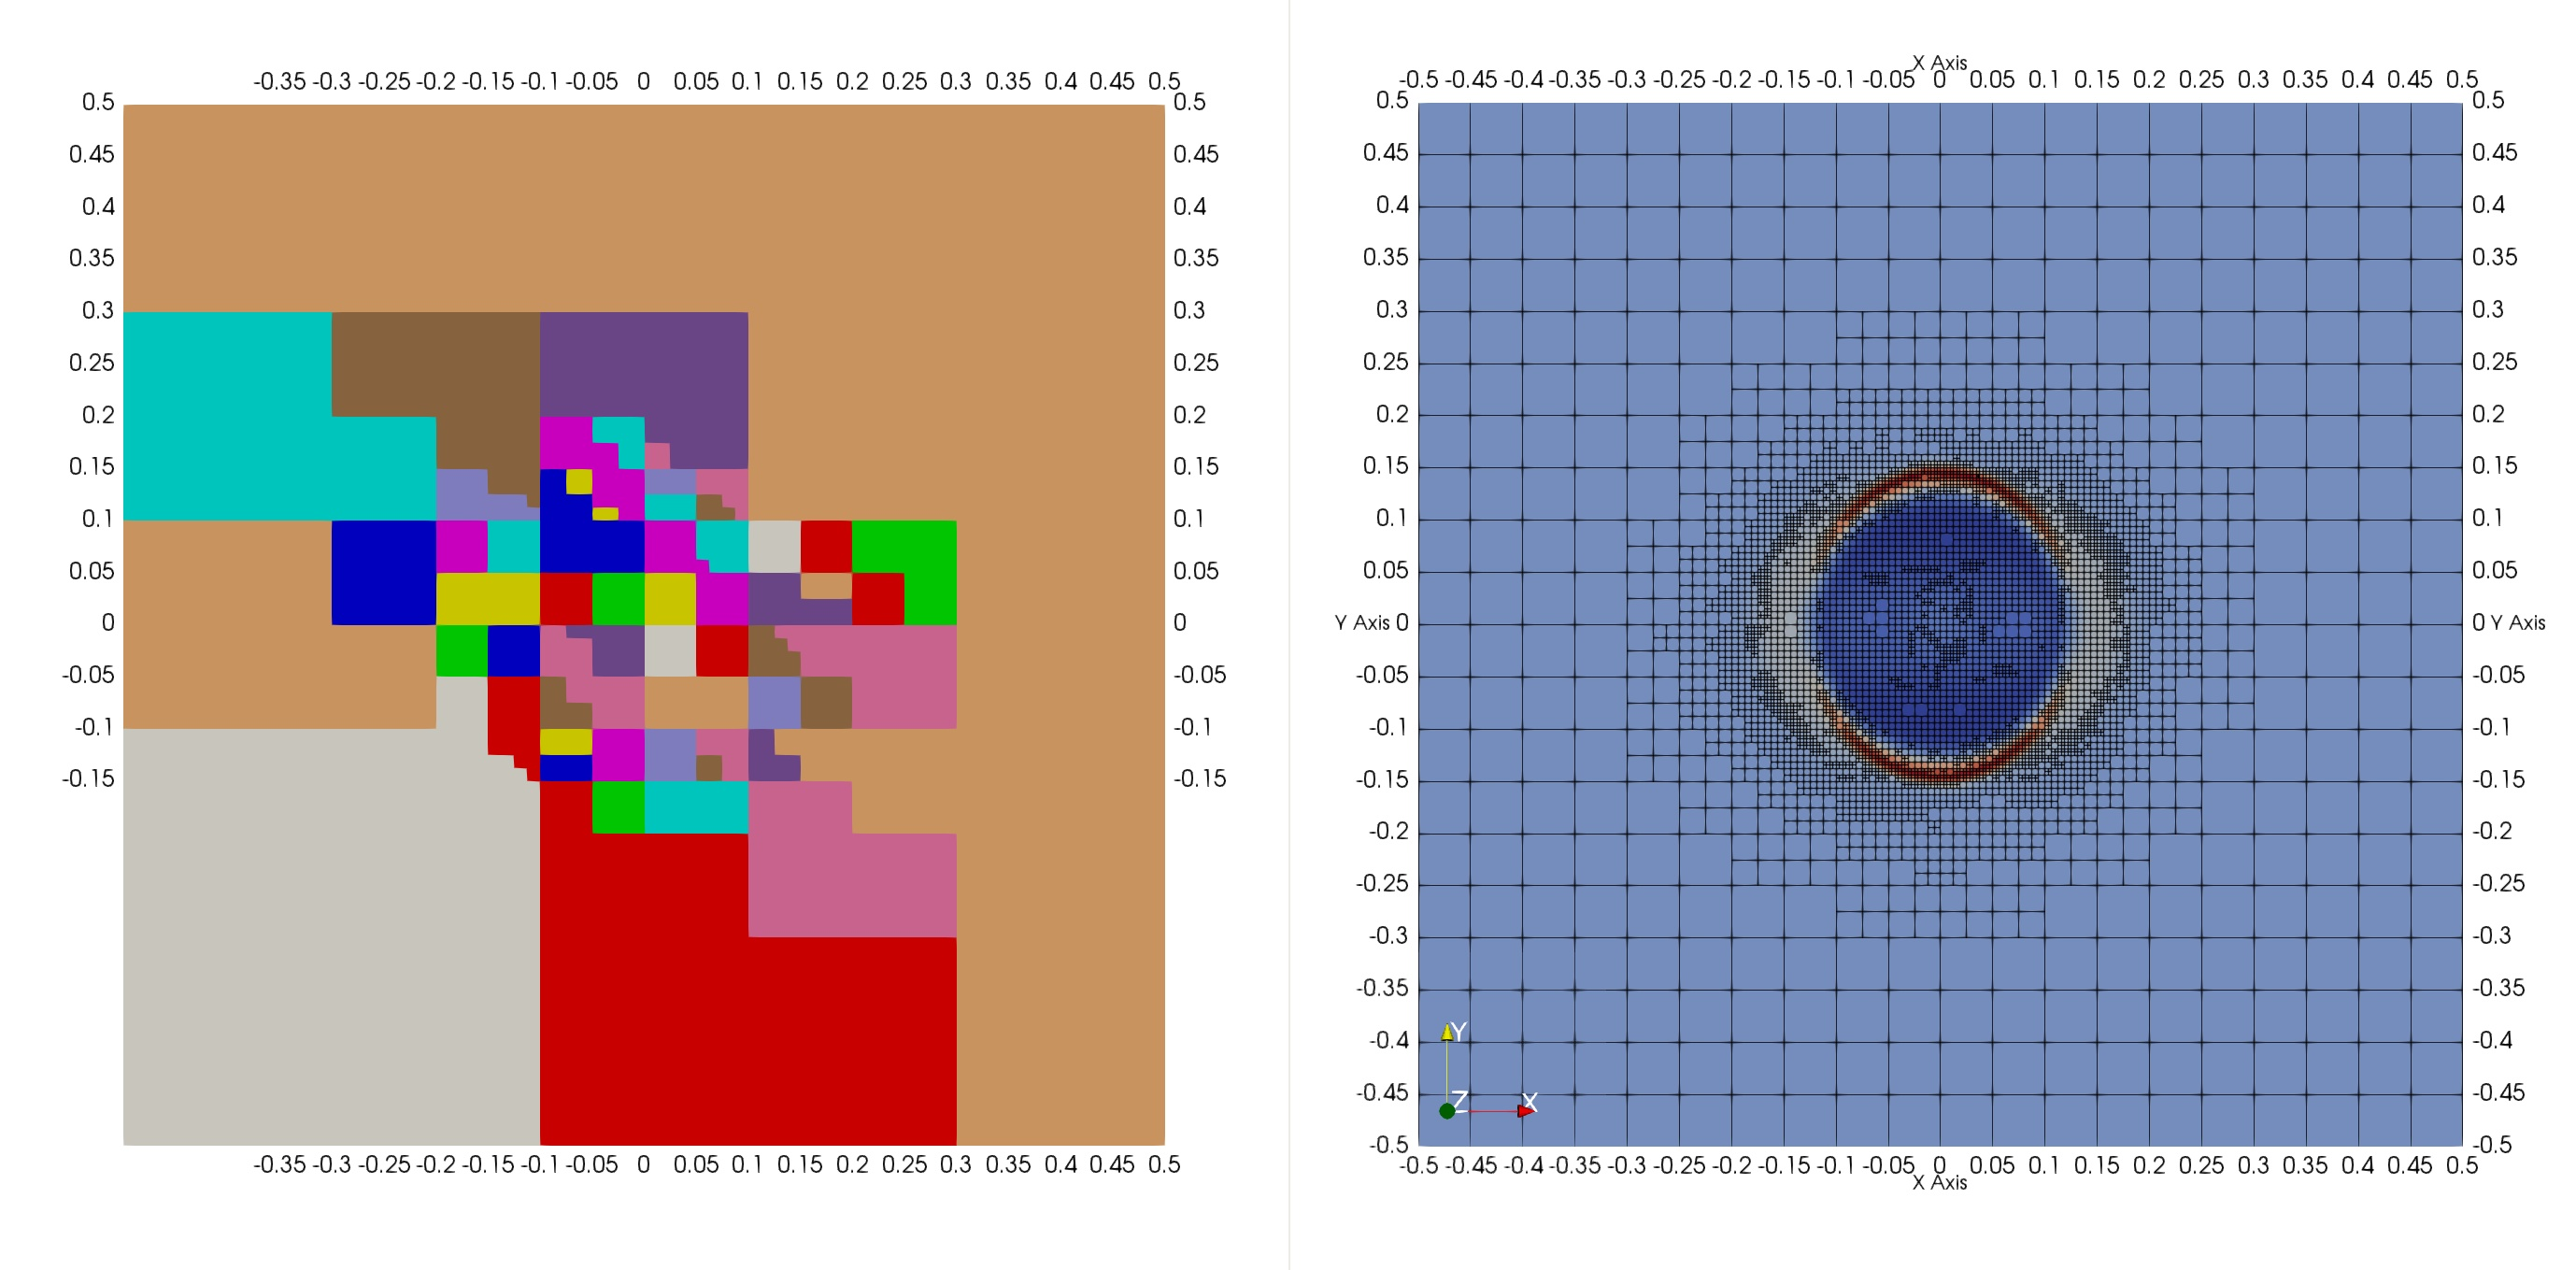
\includegraphics[width=0.87\textwidth]{img/mhd-blast/old/mya2.jpg}
	\caption{Obtained results, $t = 5\times 10^{-3}$, distribution of $\rho$ on elements in $T\lo\Omega\ro$ (right) and distribution of these elements to processors (left)}
	\label{figure:blastOldMyAdapt2}
	\end{center}
\end{figure}
\vspace{-8mm}

\begin{figure}[H]
	\begin{center}
		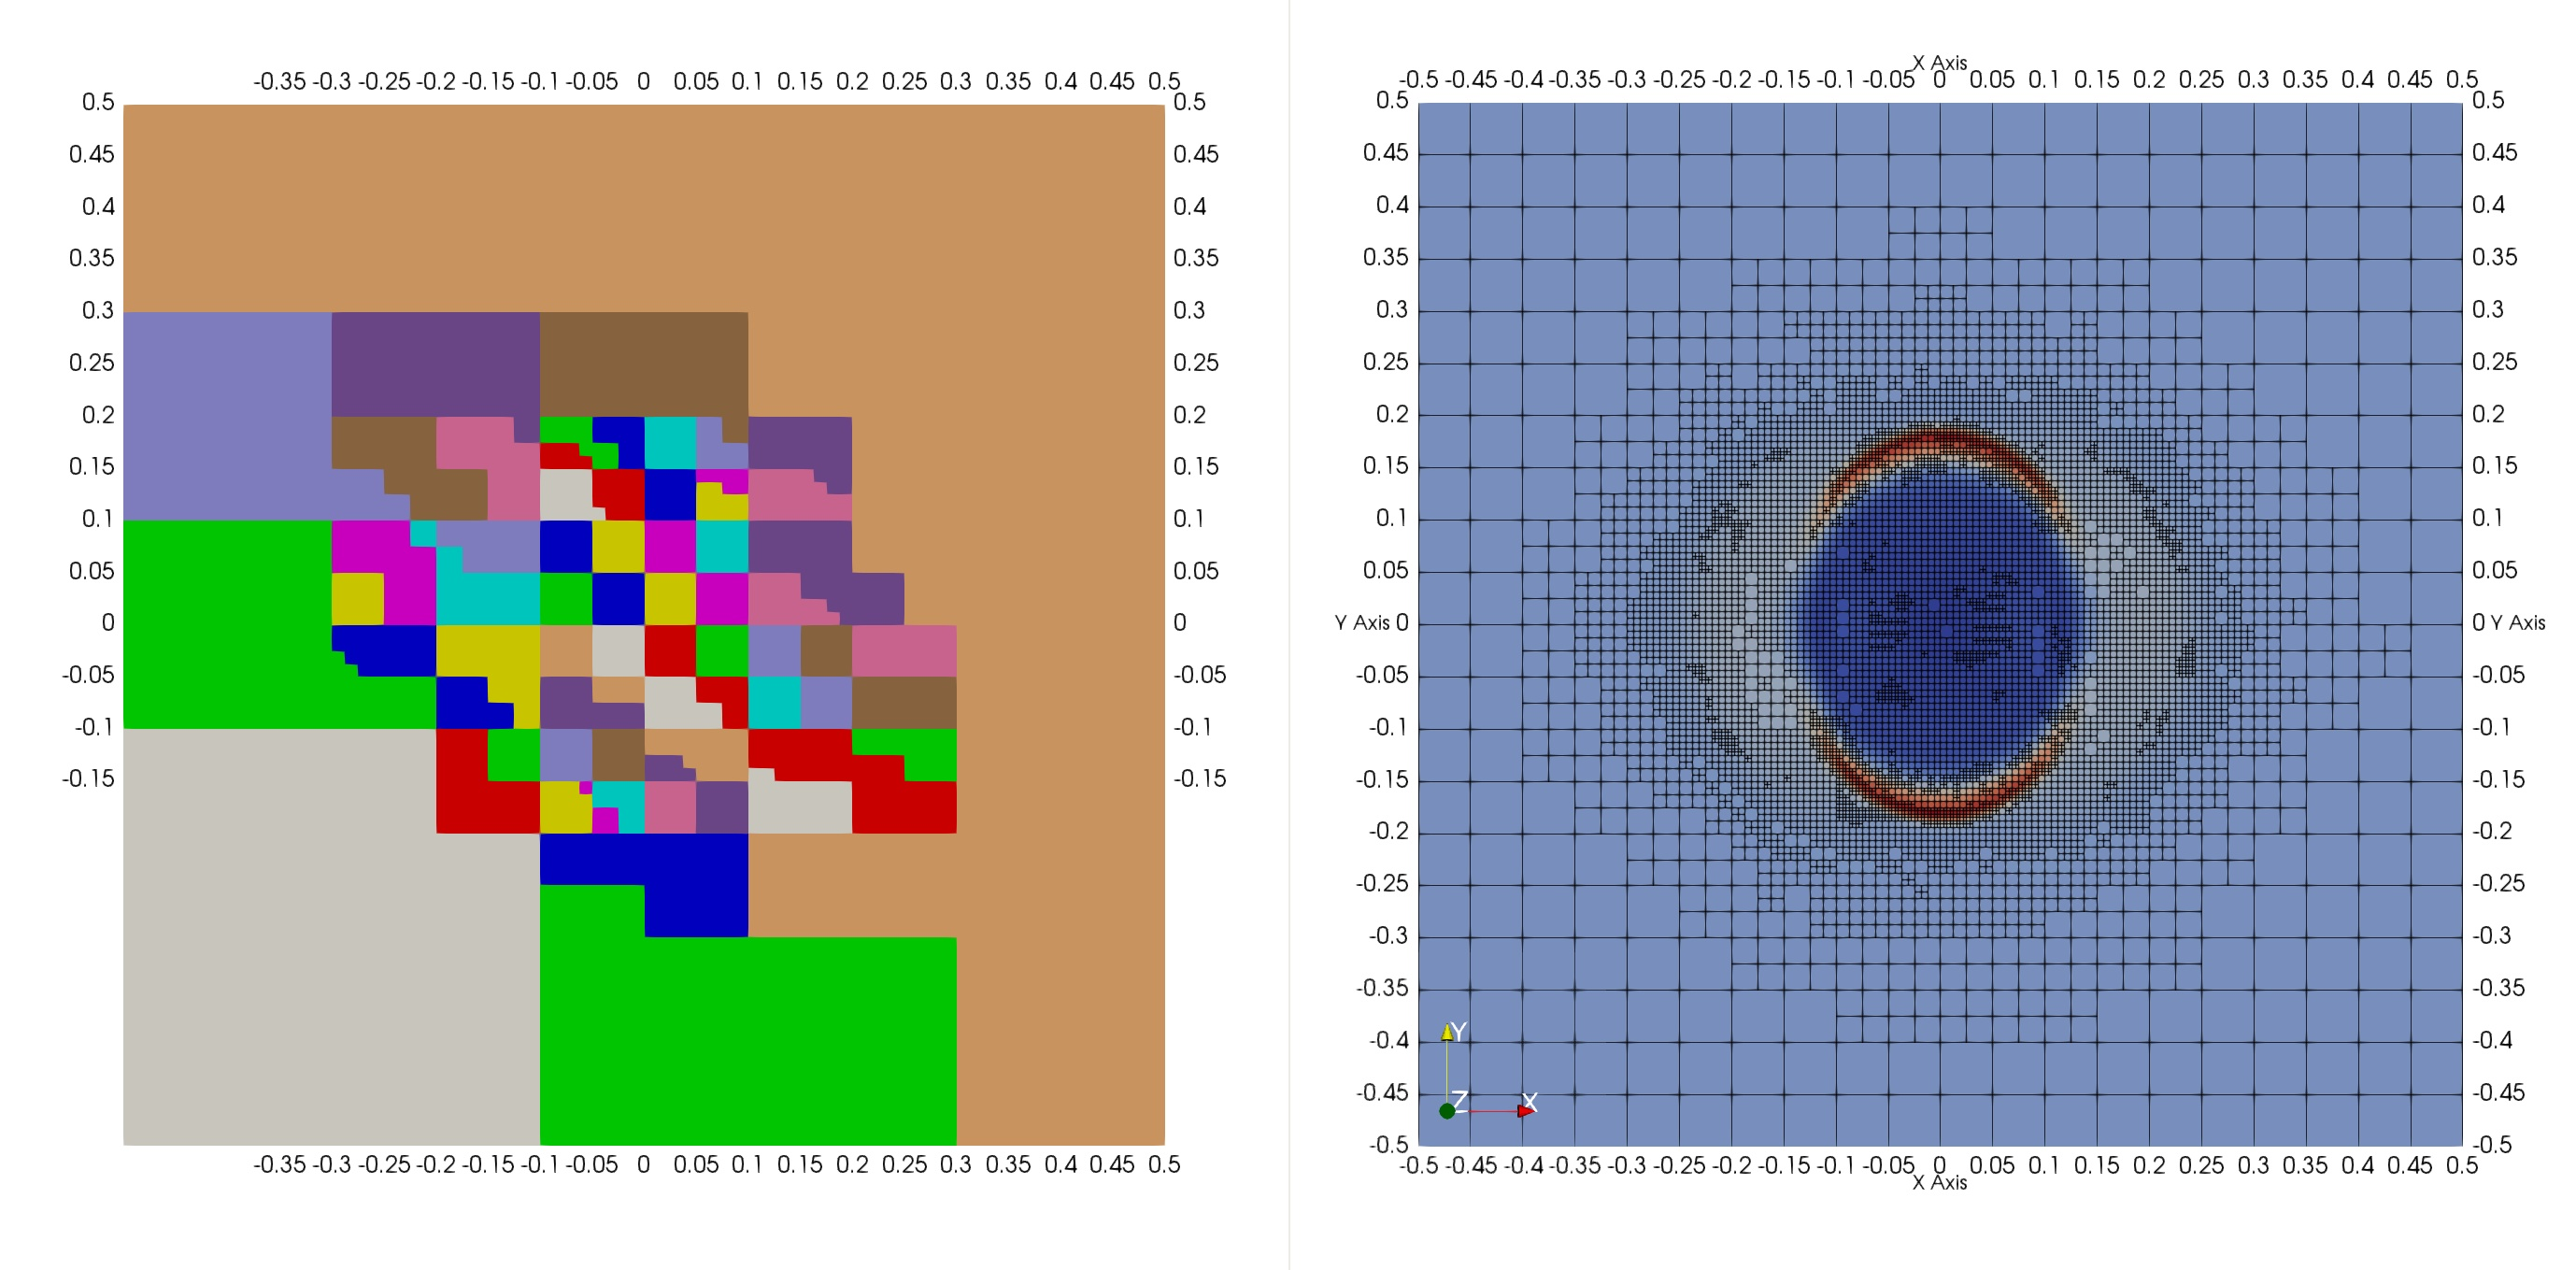
\includegraphics[width=0.87\textwidth]{img/mhd-blast/old/mya3.jpg}
	\caption{Obtained results, $t = 10\times 10^{-3}$, distribution of $\rho$ on elements in $T\lo\Omega\ro$ (right) and distribution of these elements to processors (left)}
	\label{figure:blastOldMyAdapt3}
	\end{center}
\end{figure}
\vspace{-8mm}

\begin{figure}[H]
	\begin{center}
		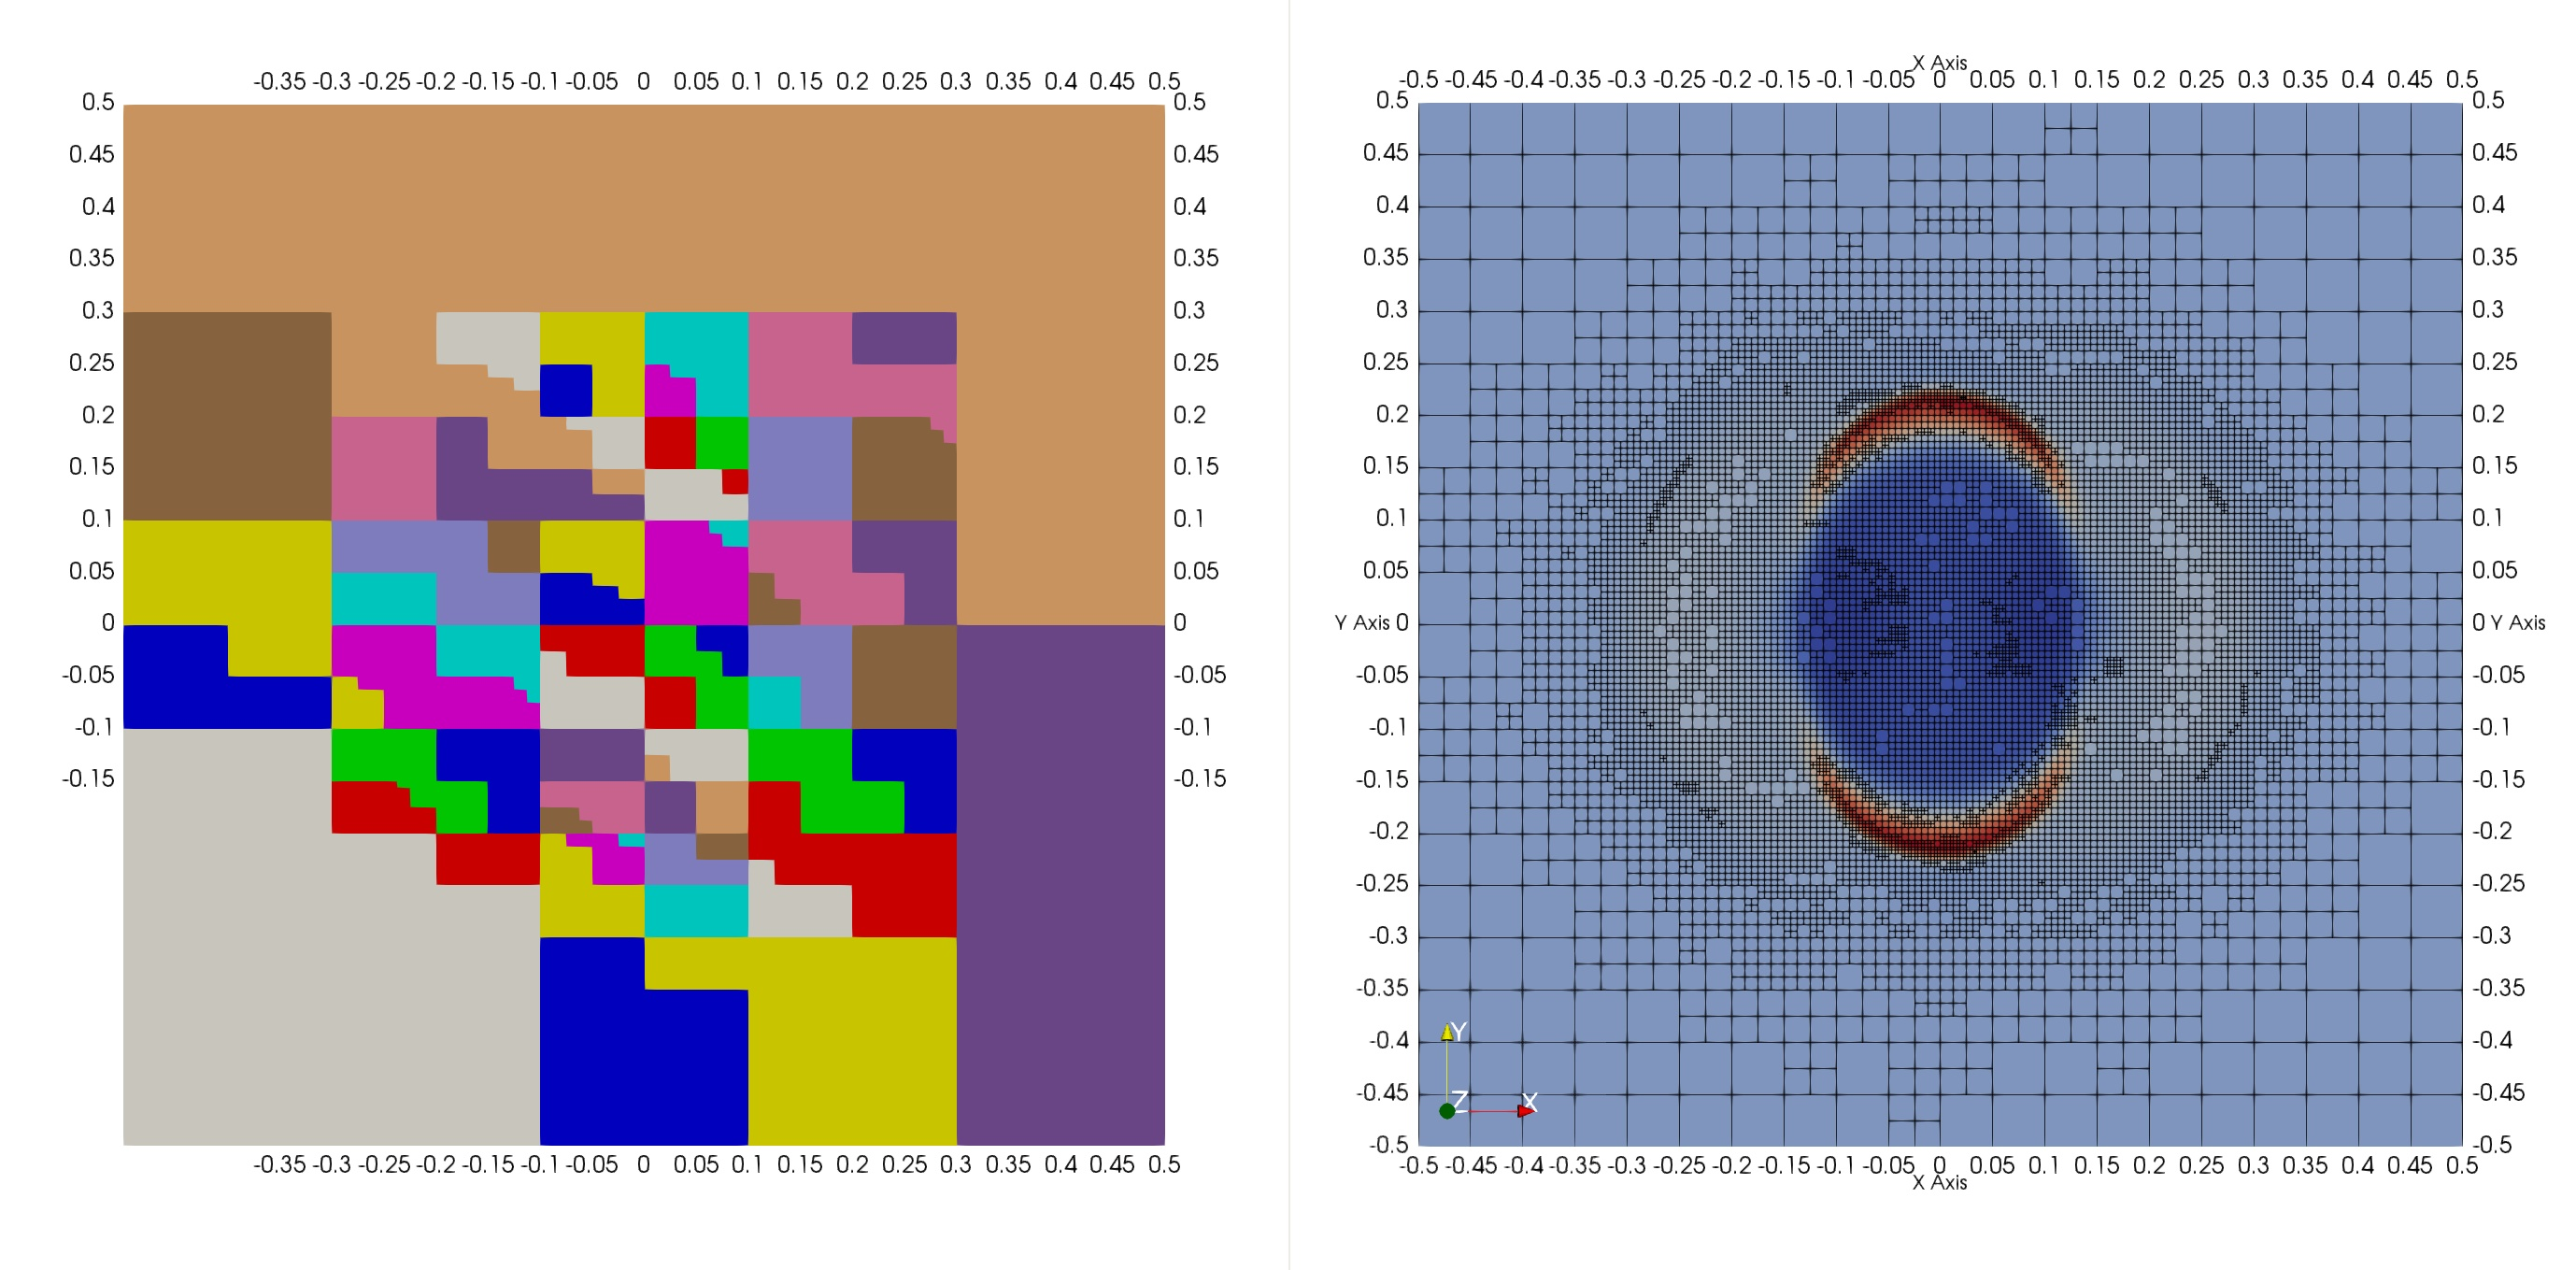
\includegraphics[width=0.87\textwidth]{img/mhd-blast/old/mya4.jpg}
	\caption{Obtained results, $t = 15\times 10^{-3}$, distribution of $\rho$ on elements in $T\lo\Omega\ro$ (right) and distribution of these elements to processors (left)}
	\label{figure:blastOldMyAdapt4}
	\end{center}
\end{figure}
\vspace{-8mm}

\begin{figure}[H]
	\begin{center}
		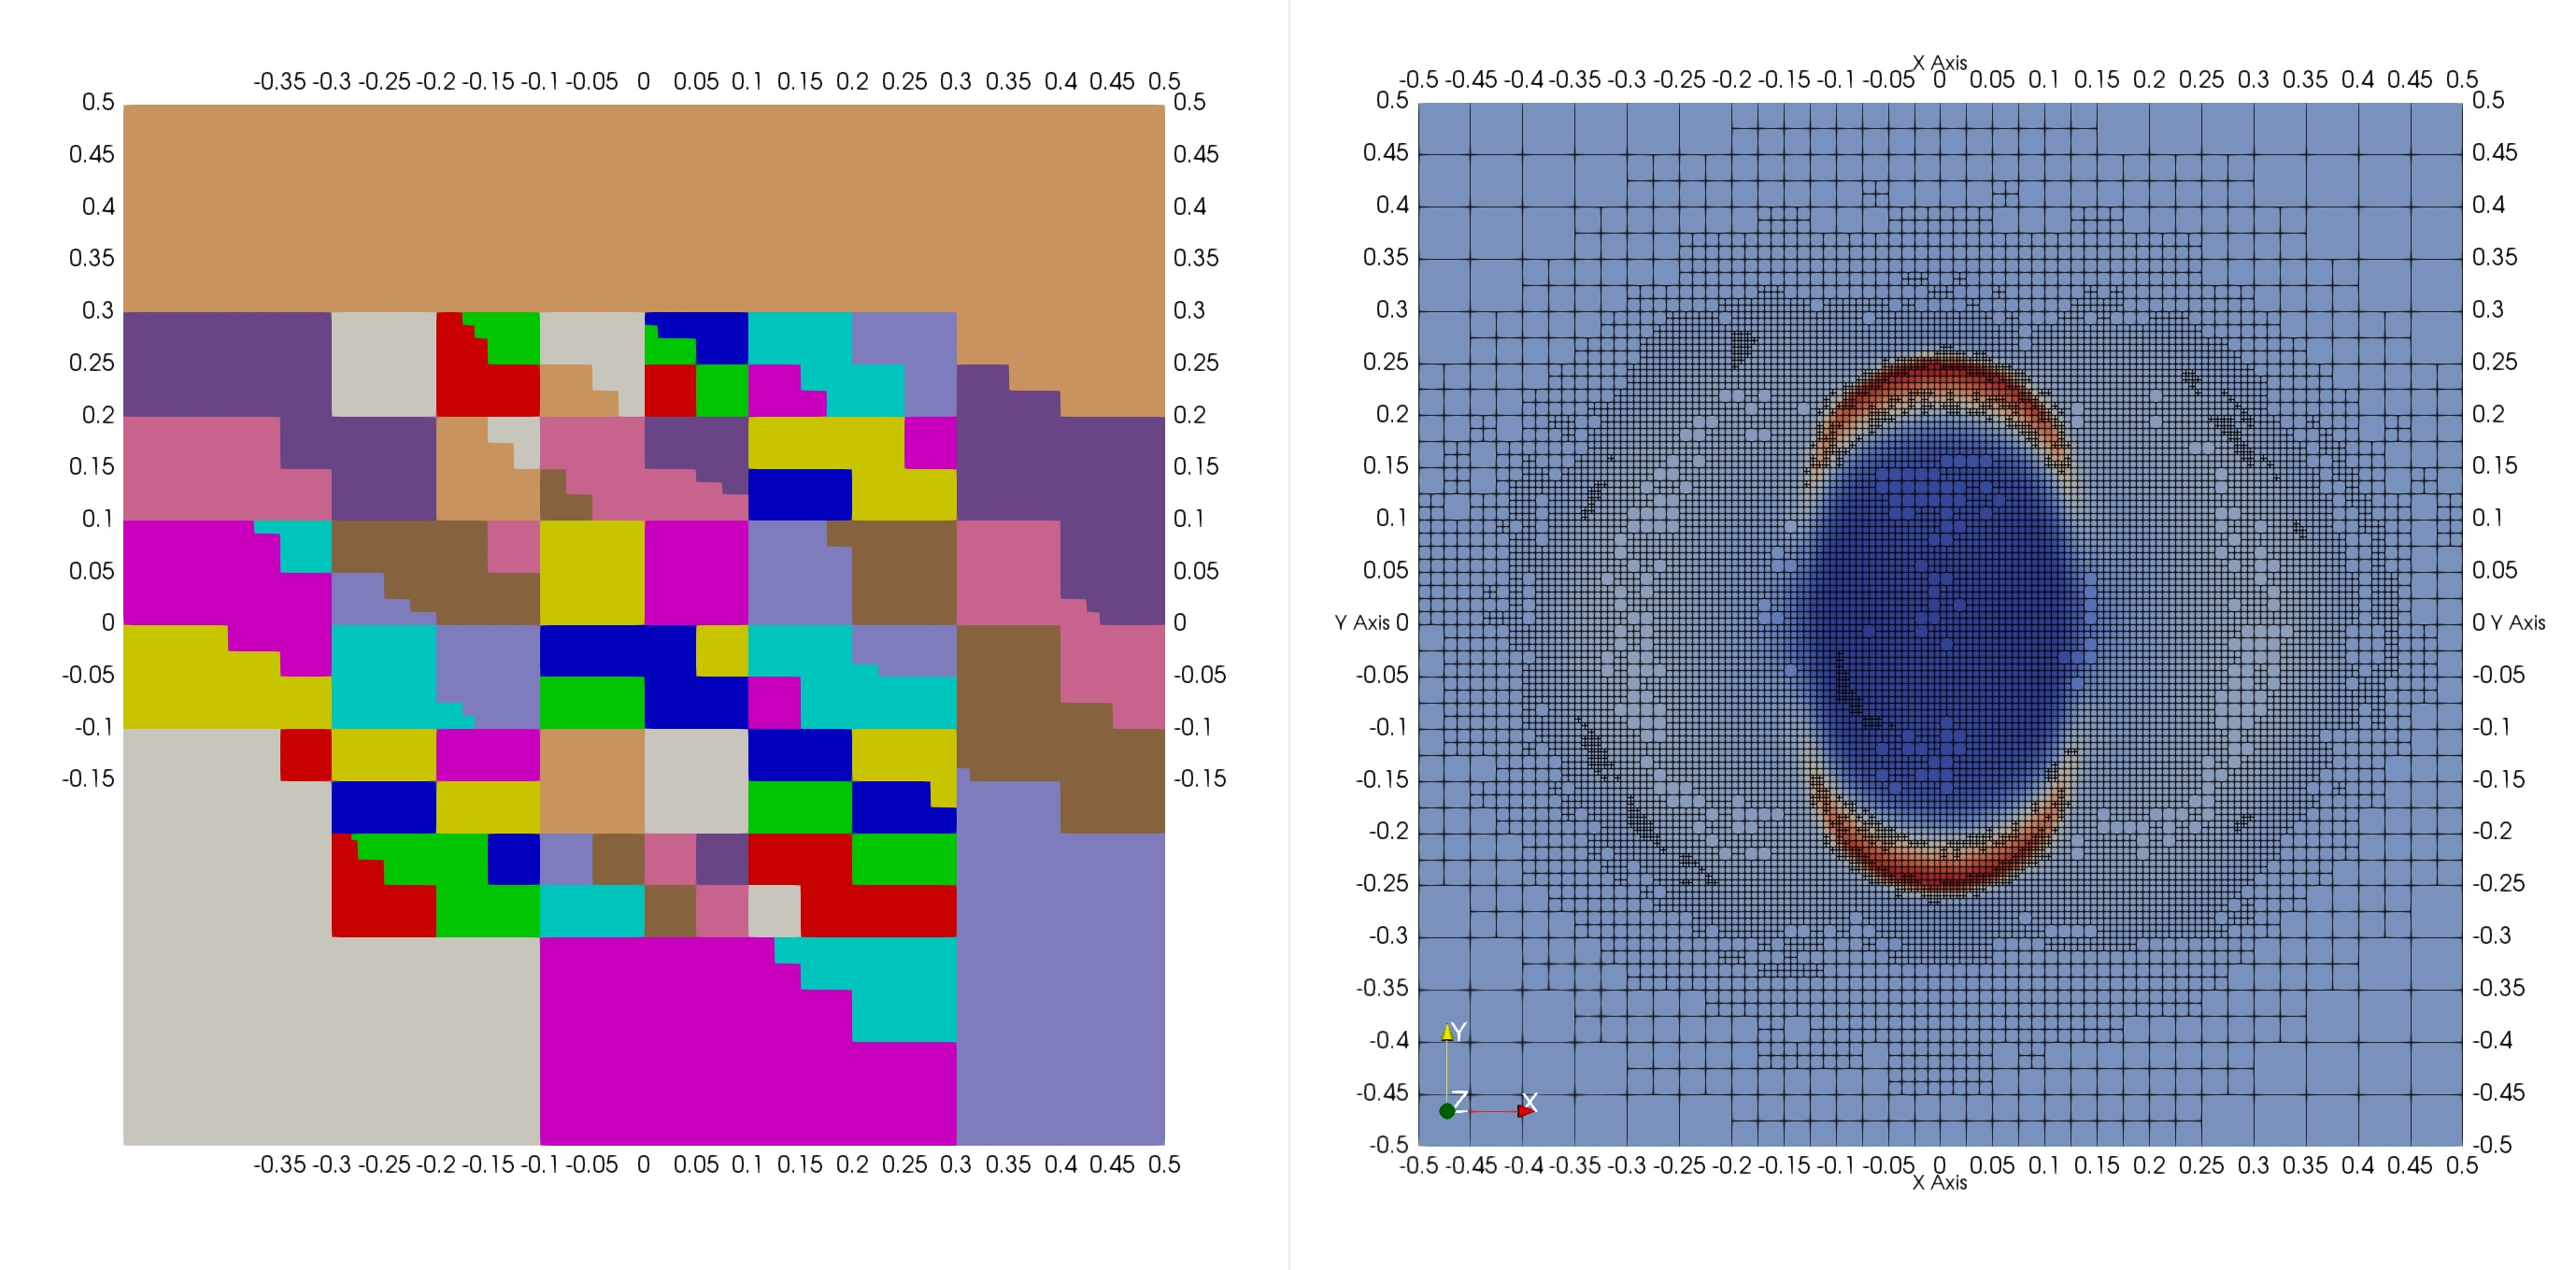
\includegraphics[width=0.87\textwidth]{img/mhd-blast/old/mya5.jpg}
	\caption{Obtained results, $t = 20\times 10^{-3}$, distribution of $\rho$ on elements in $T\lo\Omega\ro$ (right) and distribution of these elements to processors (left)}
	\label{figure:blastOldMyAdapt5}
	\end{center}
\end{figure}
\vspace{-8mm}

\begin{figure}[H]
	\begin{center}
		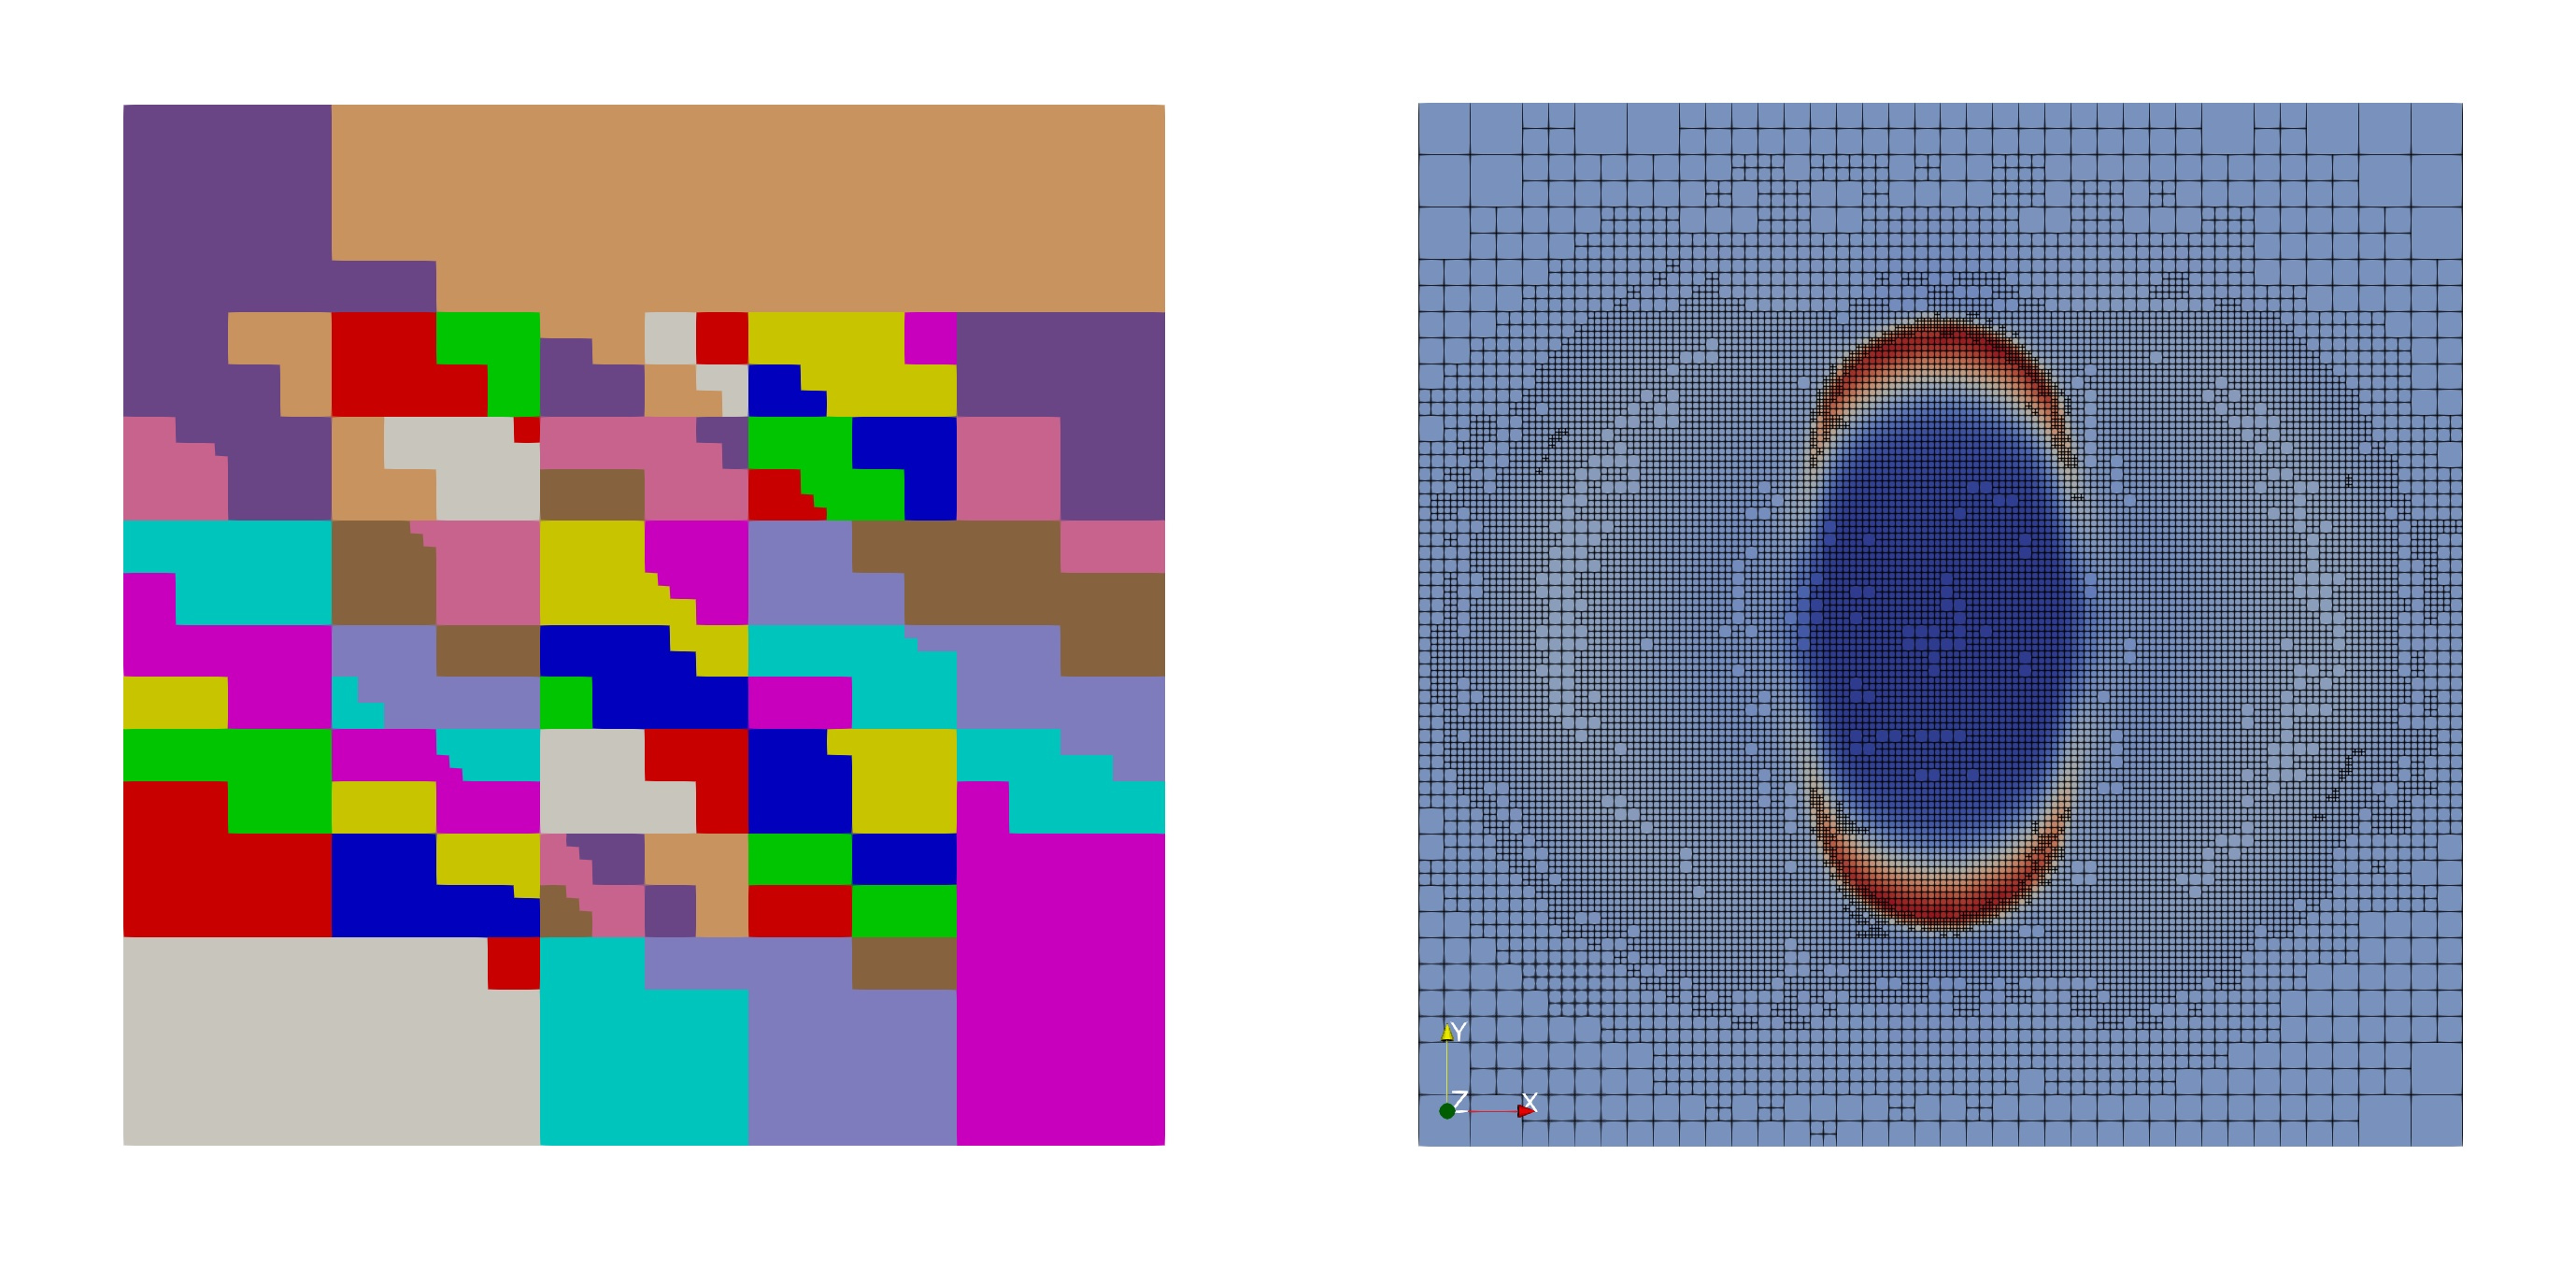
\includegraphics[width=0.87\textwidth]{img/mhd-blast/old/mya6.jpg}
	\caption{Obtained results, $t = 25\times 10^{-3}$, distribution of $\rho$ on elements in $T\lo\Omega\ro$ (right) and distribution of these elements to processors (left)}
	\label{figure:blastOldMyAdapt6}
	\end{center}
\end{figure}
\vspace{-8mm}

\subsubsection{MHD Blast - extended version}
\label{sec:blastNew}
An extended version of the benchmark has been used in \cite{blastNew1}, \cite{athenaBlast}, and a similar problem was used also in \cite{blastNew2} - the description of the benchmark is also available at:\url{http://www.astro.princeton.edu/~jstone/Athena/tests/blast/blast.html}.
In this version, the domain dimensions are set as a rectangle: $\Omega = [-0.5, 0.5] \times [-0.75, 0.75]$.
The initial conditions are a little different than in the case of \cref{mhdBlastOld}, and read:
\begin{align}
\label{mhdBlastNew}
\gamma & =  5 / 3\\ \nonumber
p_0\lo\bfx, t\ro & =  10\ \ \text{for}\ \left|\bfx\right| < 0.1\\ \nonumber
p_0\lo\bfx, t\ro & =  0.1\ \ \text{for}\ \left|\bfx\right| \geq 0.1\\ \nonumber
\rho\lo\bfx, t = 0\ro & =  1,\\ \nonumber
p\lo\bfx, t = 0\ro & =  p_0\lo\bfx, t\ro,\\ \nonumber
\bfu_1\lo\bfx, t = 0\ro & =  0,\\ \nonumber	
\bfu_2\lo\bfx, t = 0\ro & =  0,\\ \nonumber
\bfu_3\lo\bfx, t = 0\ro & =  0,\\ \nonumber
\bfB_1\lo\bfx, t = 0\ro & =  \frac{1}{\sqrt{2}},\\ \nonumber
\bfB_2\lo\bfx, t = 0\ro & =  \frac{1}{\sqrt{2}},\\ \nonumber
\bfB_3\lo\bfx, t = 0\ro & =  0,
\end{align}
with periodic boundary conditions on the top-bottom, and left-right parts of the boundary. That is, with respect to \cref{periodicMapping}, the two pairs $\Gamma_1, \Gamma_2, \Gamma_1^{'}, \Gamma_2^{'}$ are specified as follows:
\begin{align}
\Gamma_1 & = \left\{-0.5\right\} \times [-0.75, 0.75],\\
\Gamma_2 & = \left\{0.5\right\} \times [-0.75, 0.75],
\end{align}
and
\begin{align}
\Gamma_1^{'} & = [-0.5, 0.5] \times \left\{-0.75\right\},\\
\Gamma_2^{'} & = [-0.5, 0.5] \times \left\{0.75\right\}.
\end{align}

The solution image taken from \cite{blastNew1} is for comparison in \cref{figure:blastRef}.

\subsubsection{Results}
The first set of results are from calculations using piecewise-constant elements, on three successively uniformly refined meshes. The meshes used for computations \crefrange{figure:blastNew01}{figure:blastNew06} contained:
\begin{itemize}
\item $100 \times 150$ elements (left)
\item $200 \times 300$ elements (middle)
\item $400 \times 600$ elements (right)
\end{itemize}

\begin{figure}[H]
	\begin{center}
		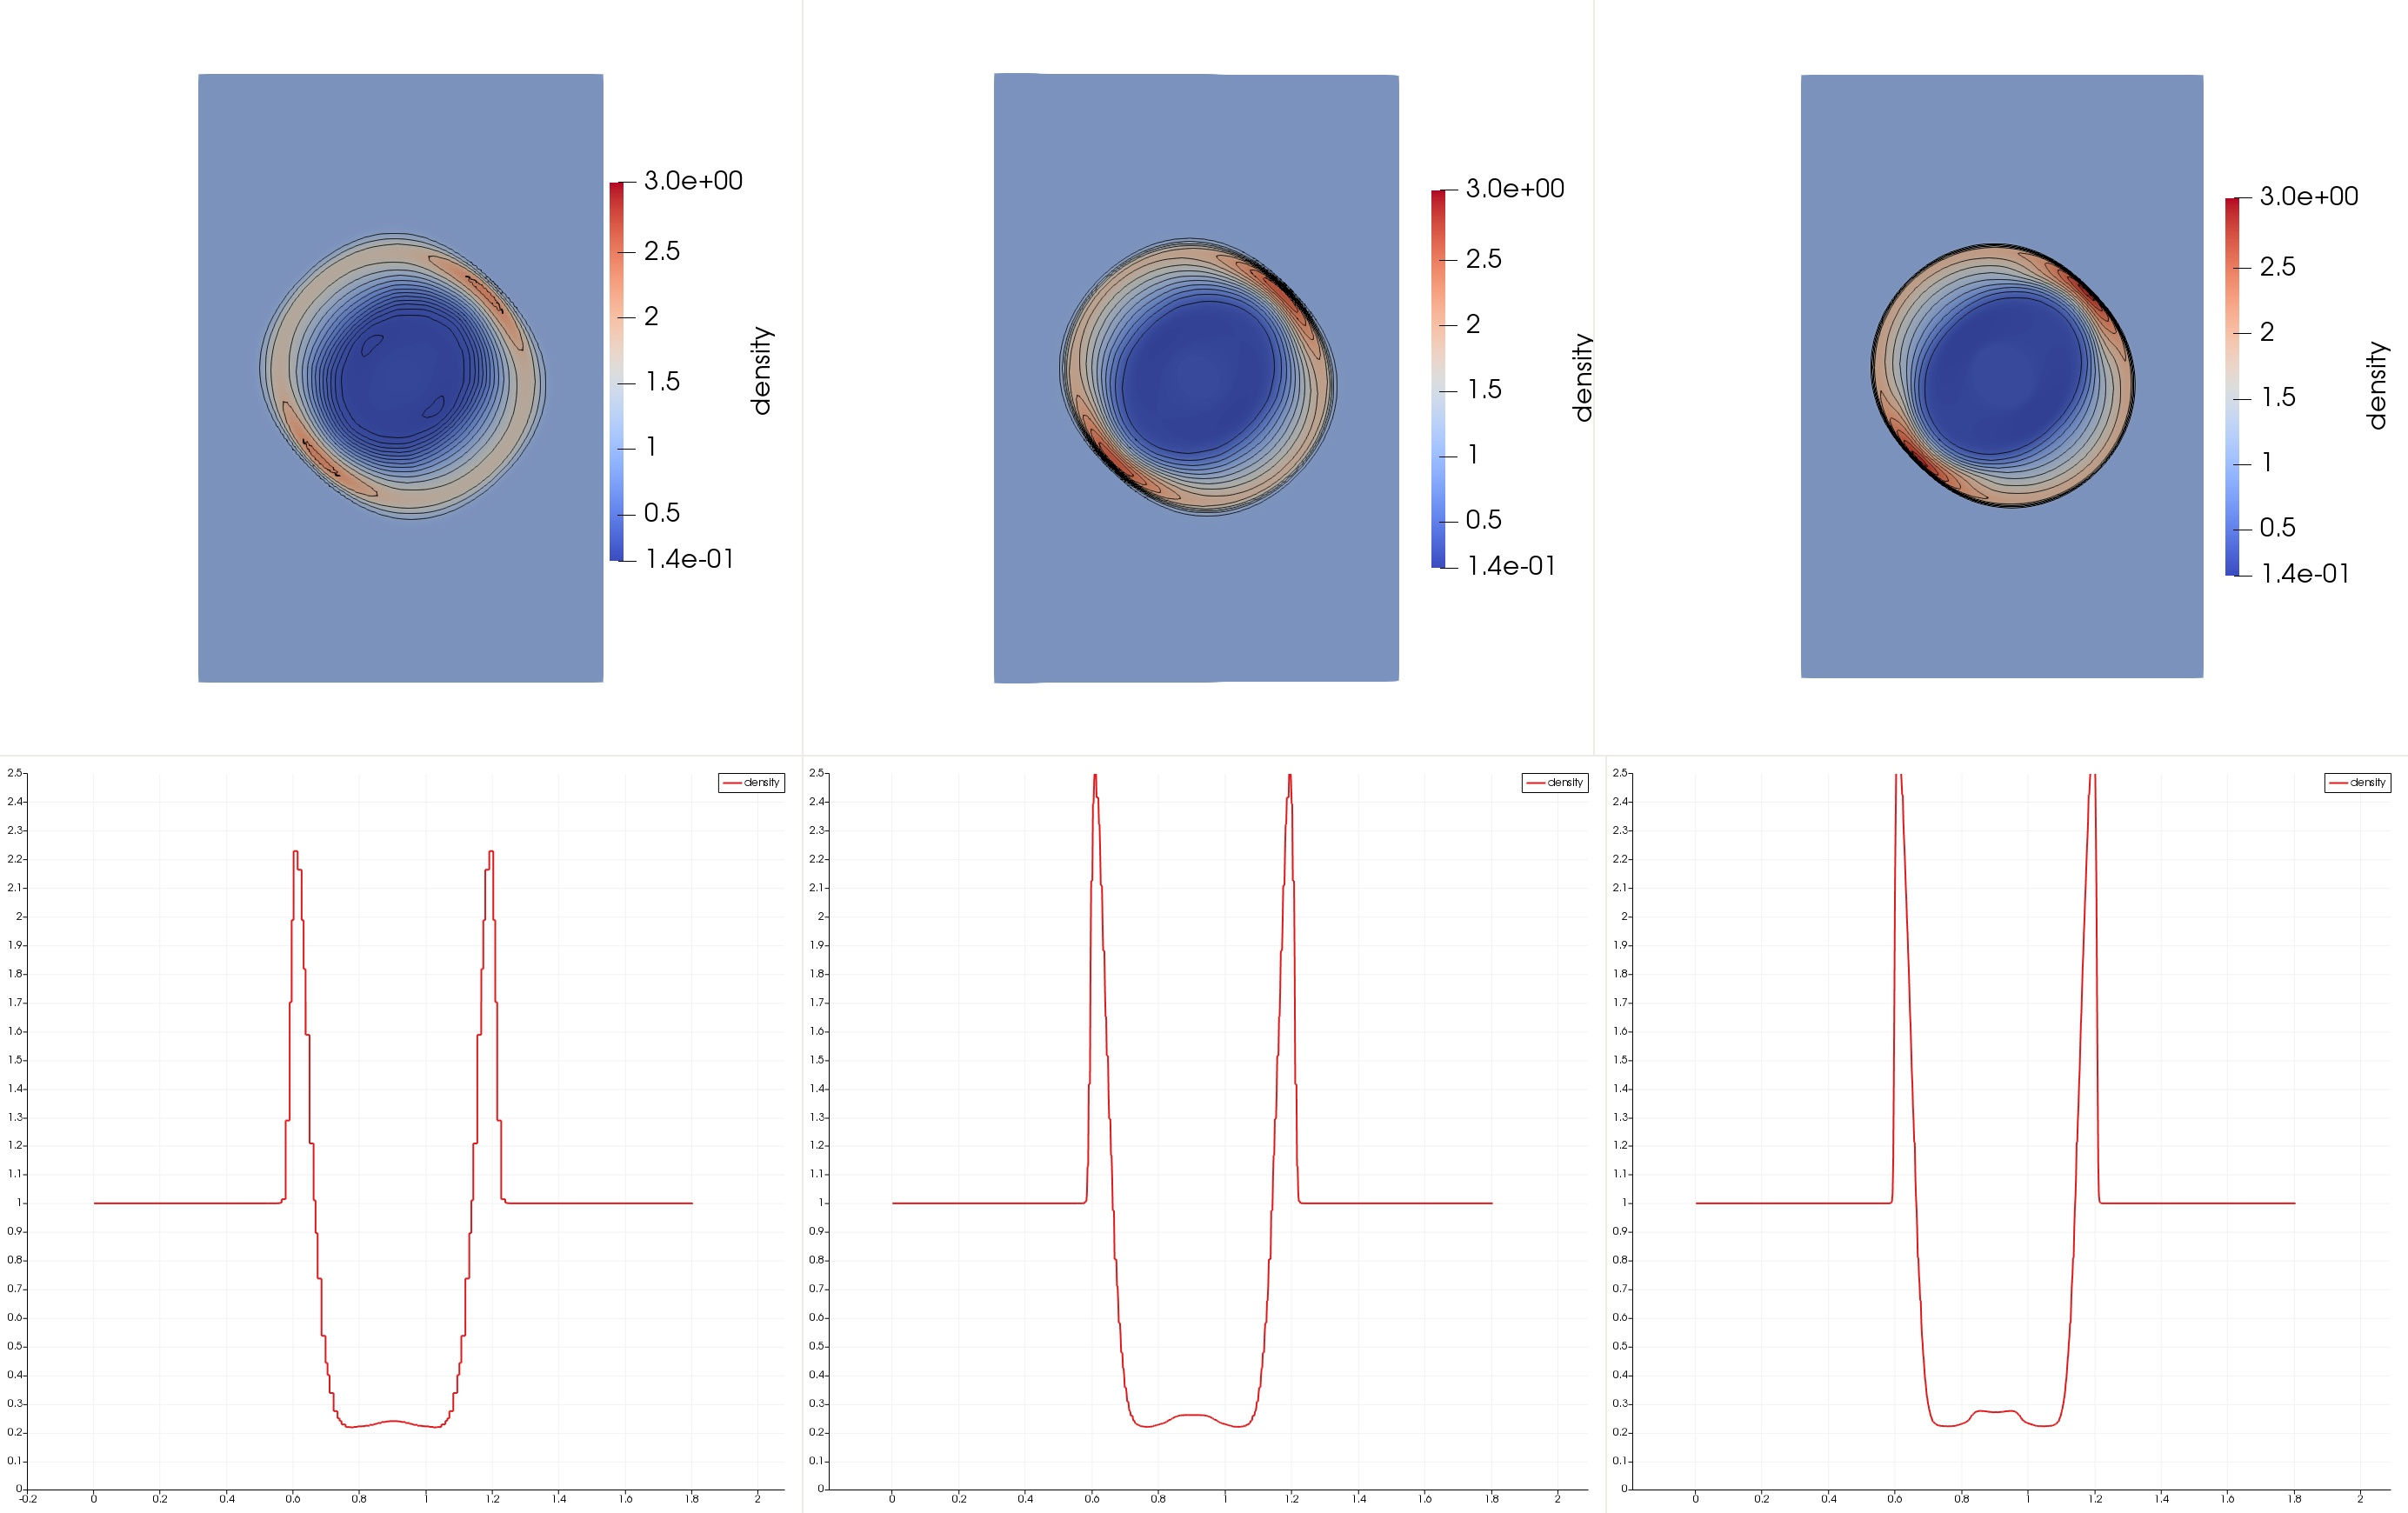
\includegraphics[width=0.95\textwidth]{img/mhd-blast/new/blast,noadapt1.jpg}
	\caption{Obtained results, $t \approx 0.1$, distribution of $\rho$ (top), with line distribution along bottom-left $\rightarrow$ top-right diagonal (bottom)}
	\label{figure:blastNew01}
	\end{center}
\end{figure}
\vspace{-8mm}

\begin{figure}[H]
	\begin{center}
		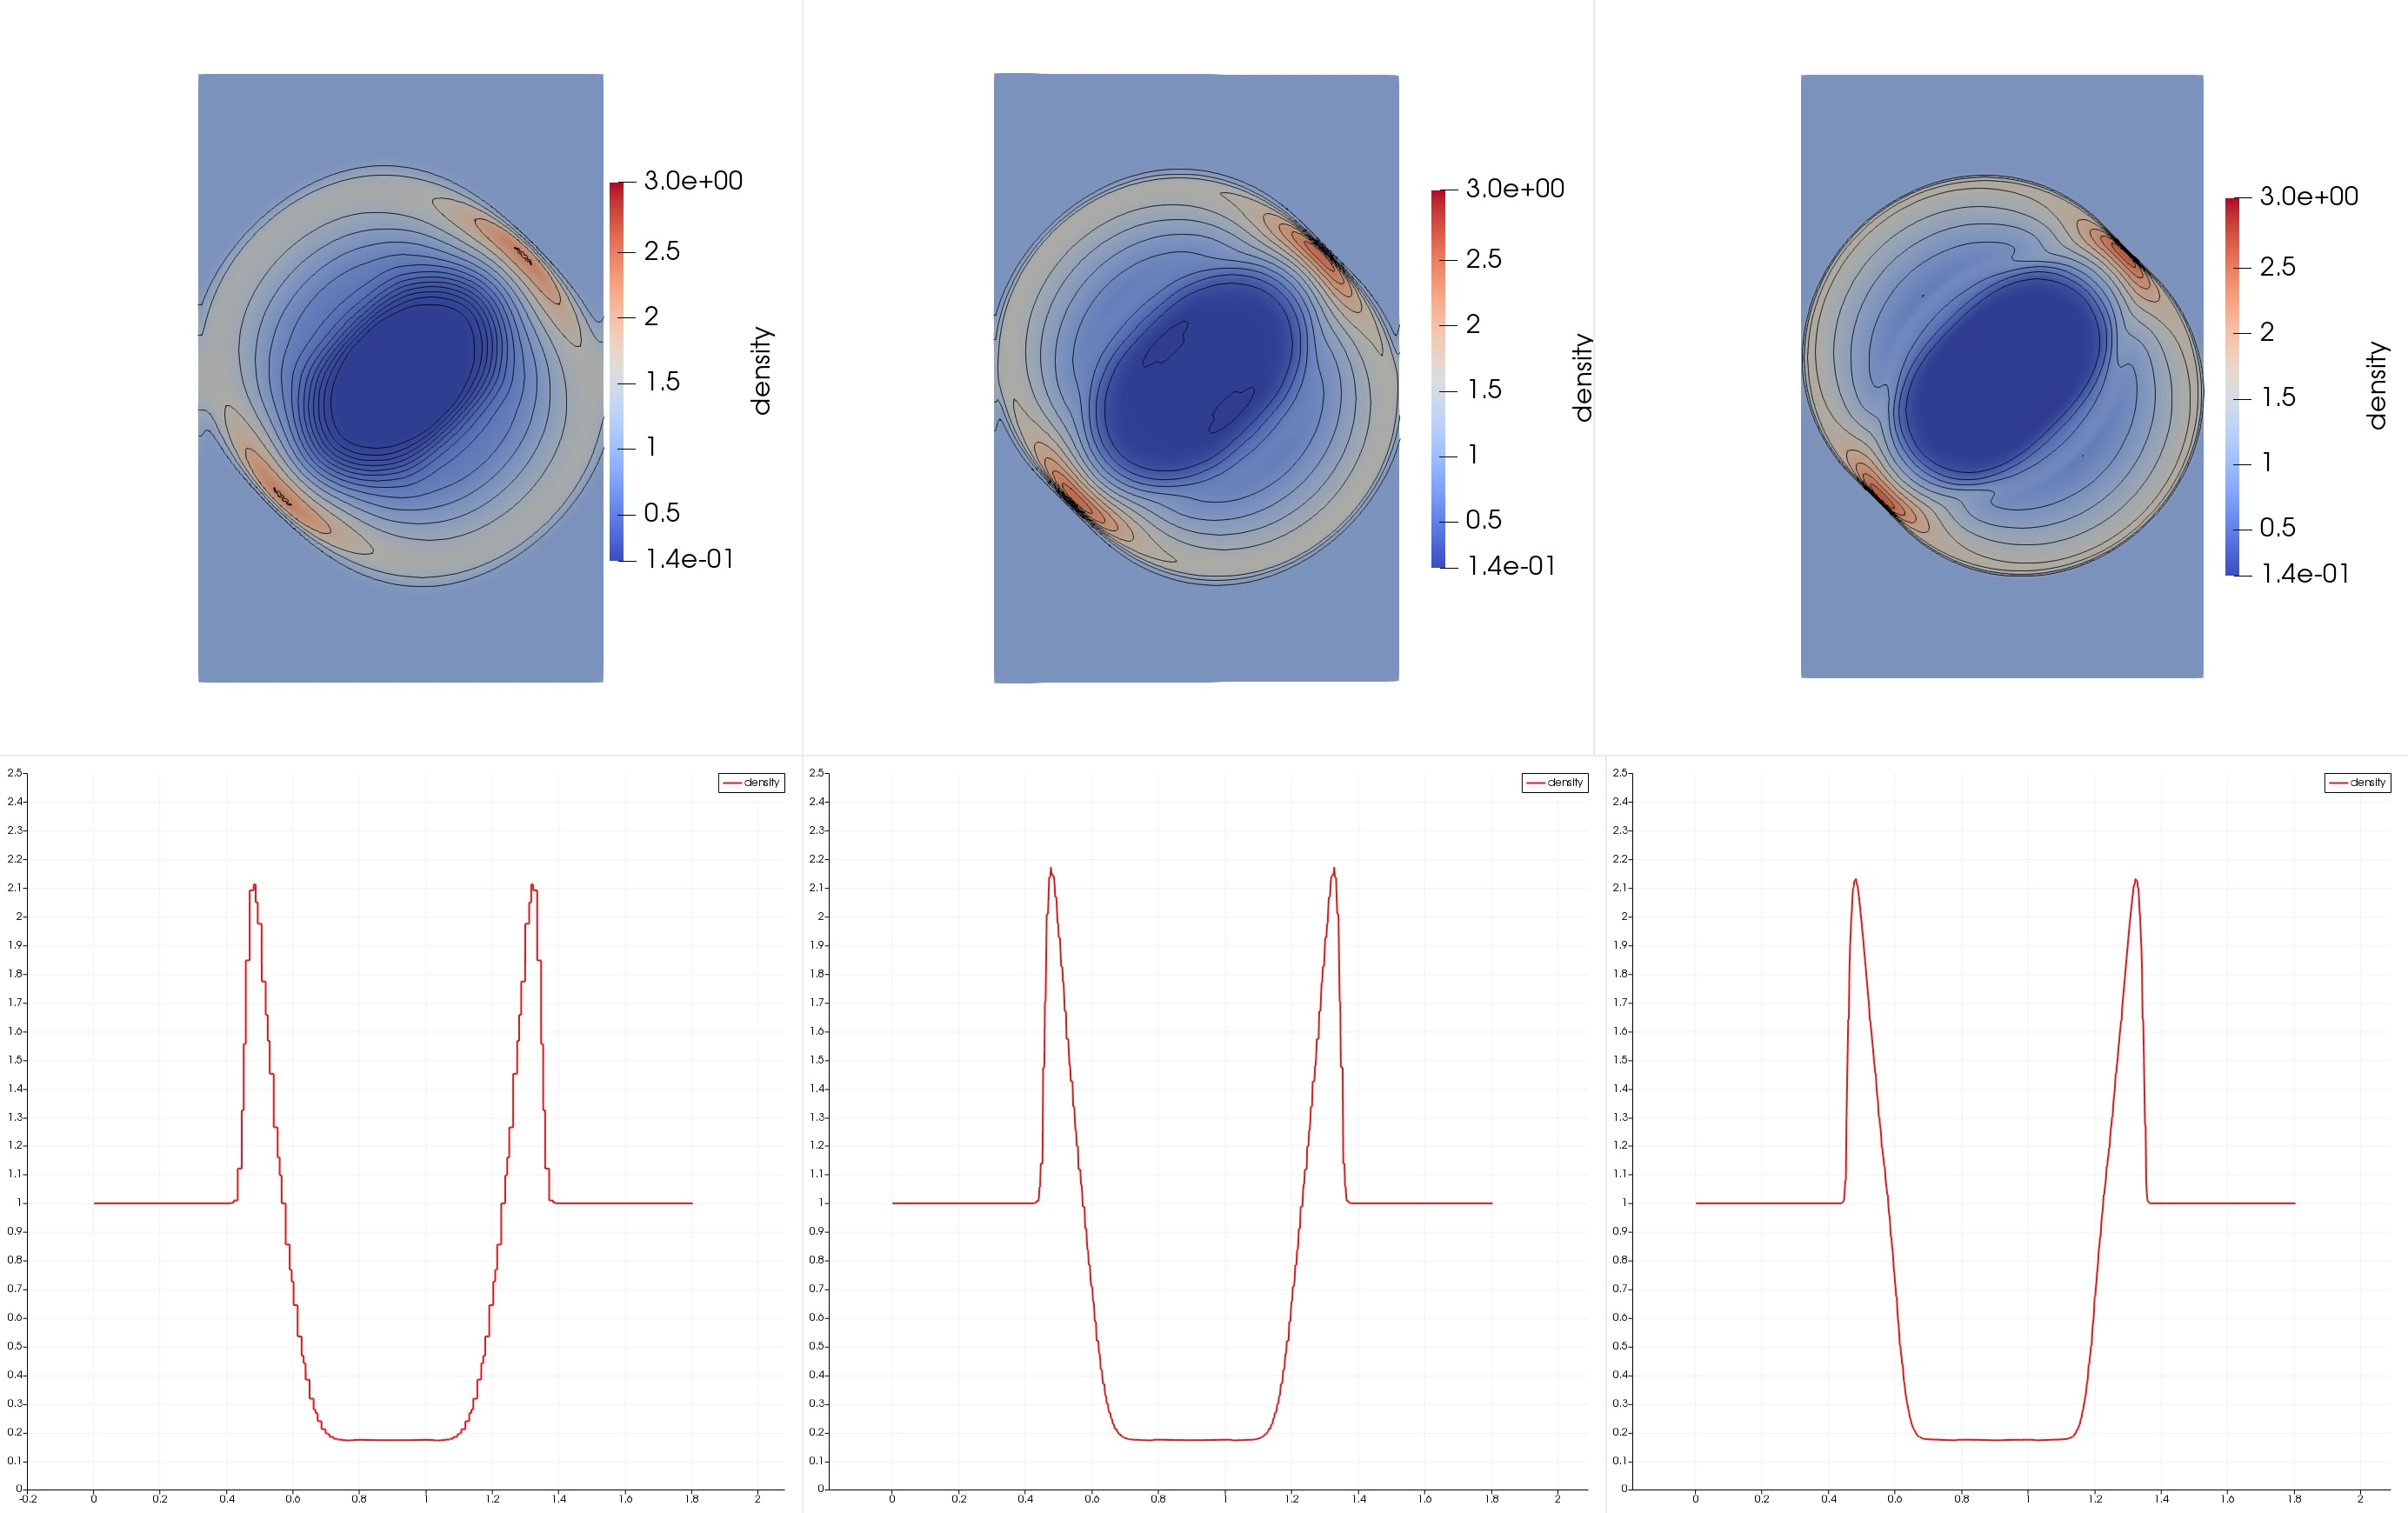
\includegraphics[width=0.95\textwidth]{img/mhd-blast/new/blast,noadapt3.jpg}
	\caption{Obtained results, $t = \approx 0.2$, distribution of $\rho$ (top), with line distribution along bottom-left $\rightarrow$ top-right diagonal (bottom)}
	\label{figure:blastNew02}
	\end{center}
\end{figure}
\vspace{-8mm}

\begin{figure}[H]
	\begin{center}
		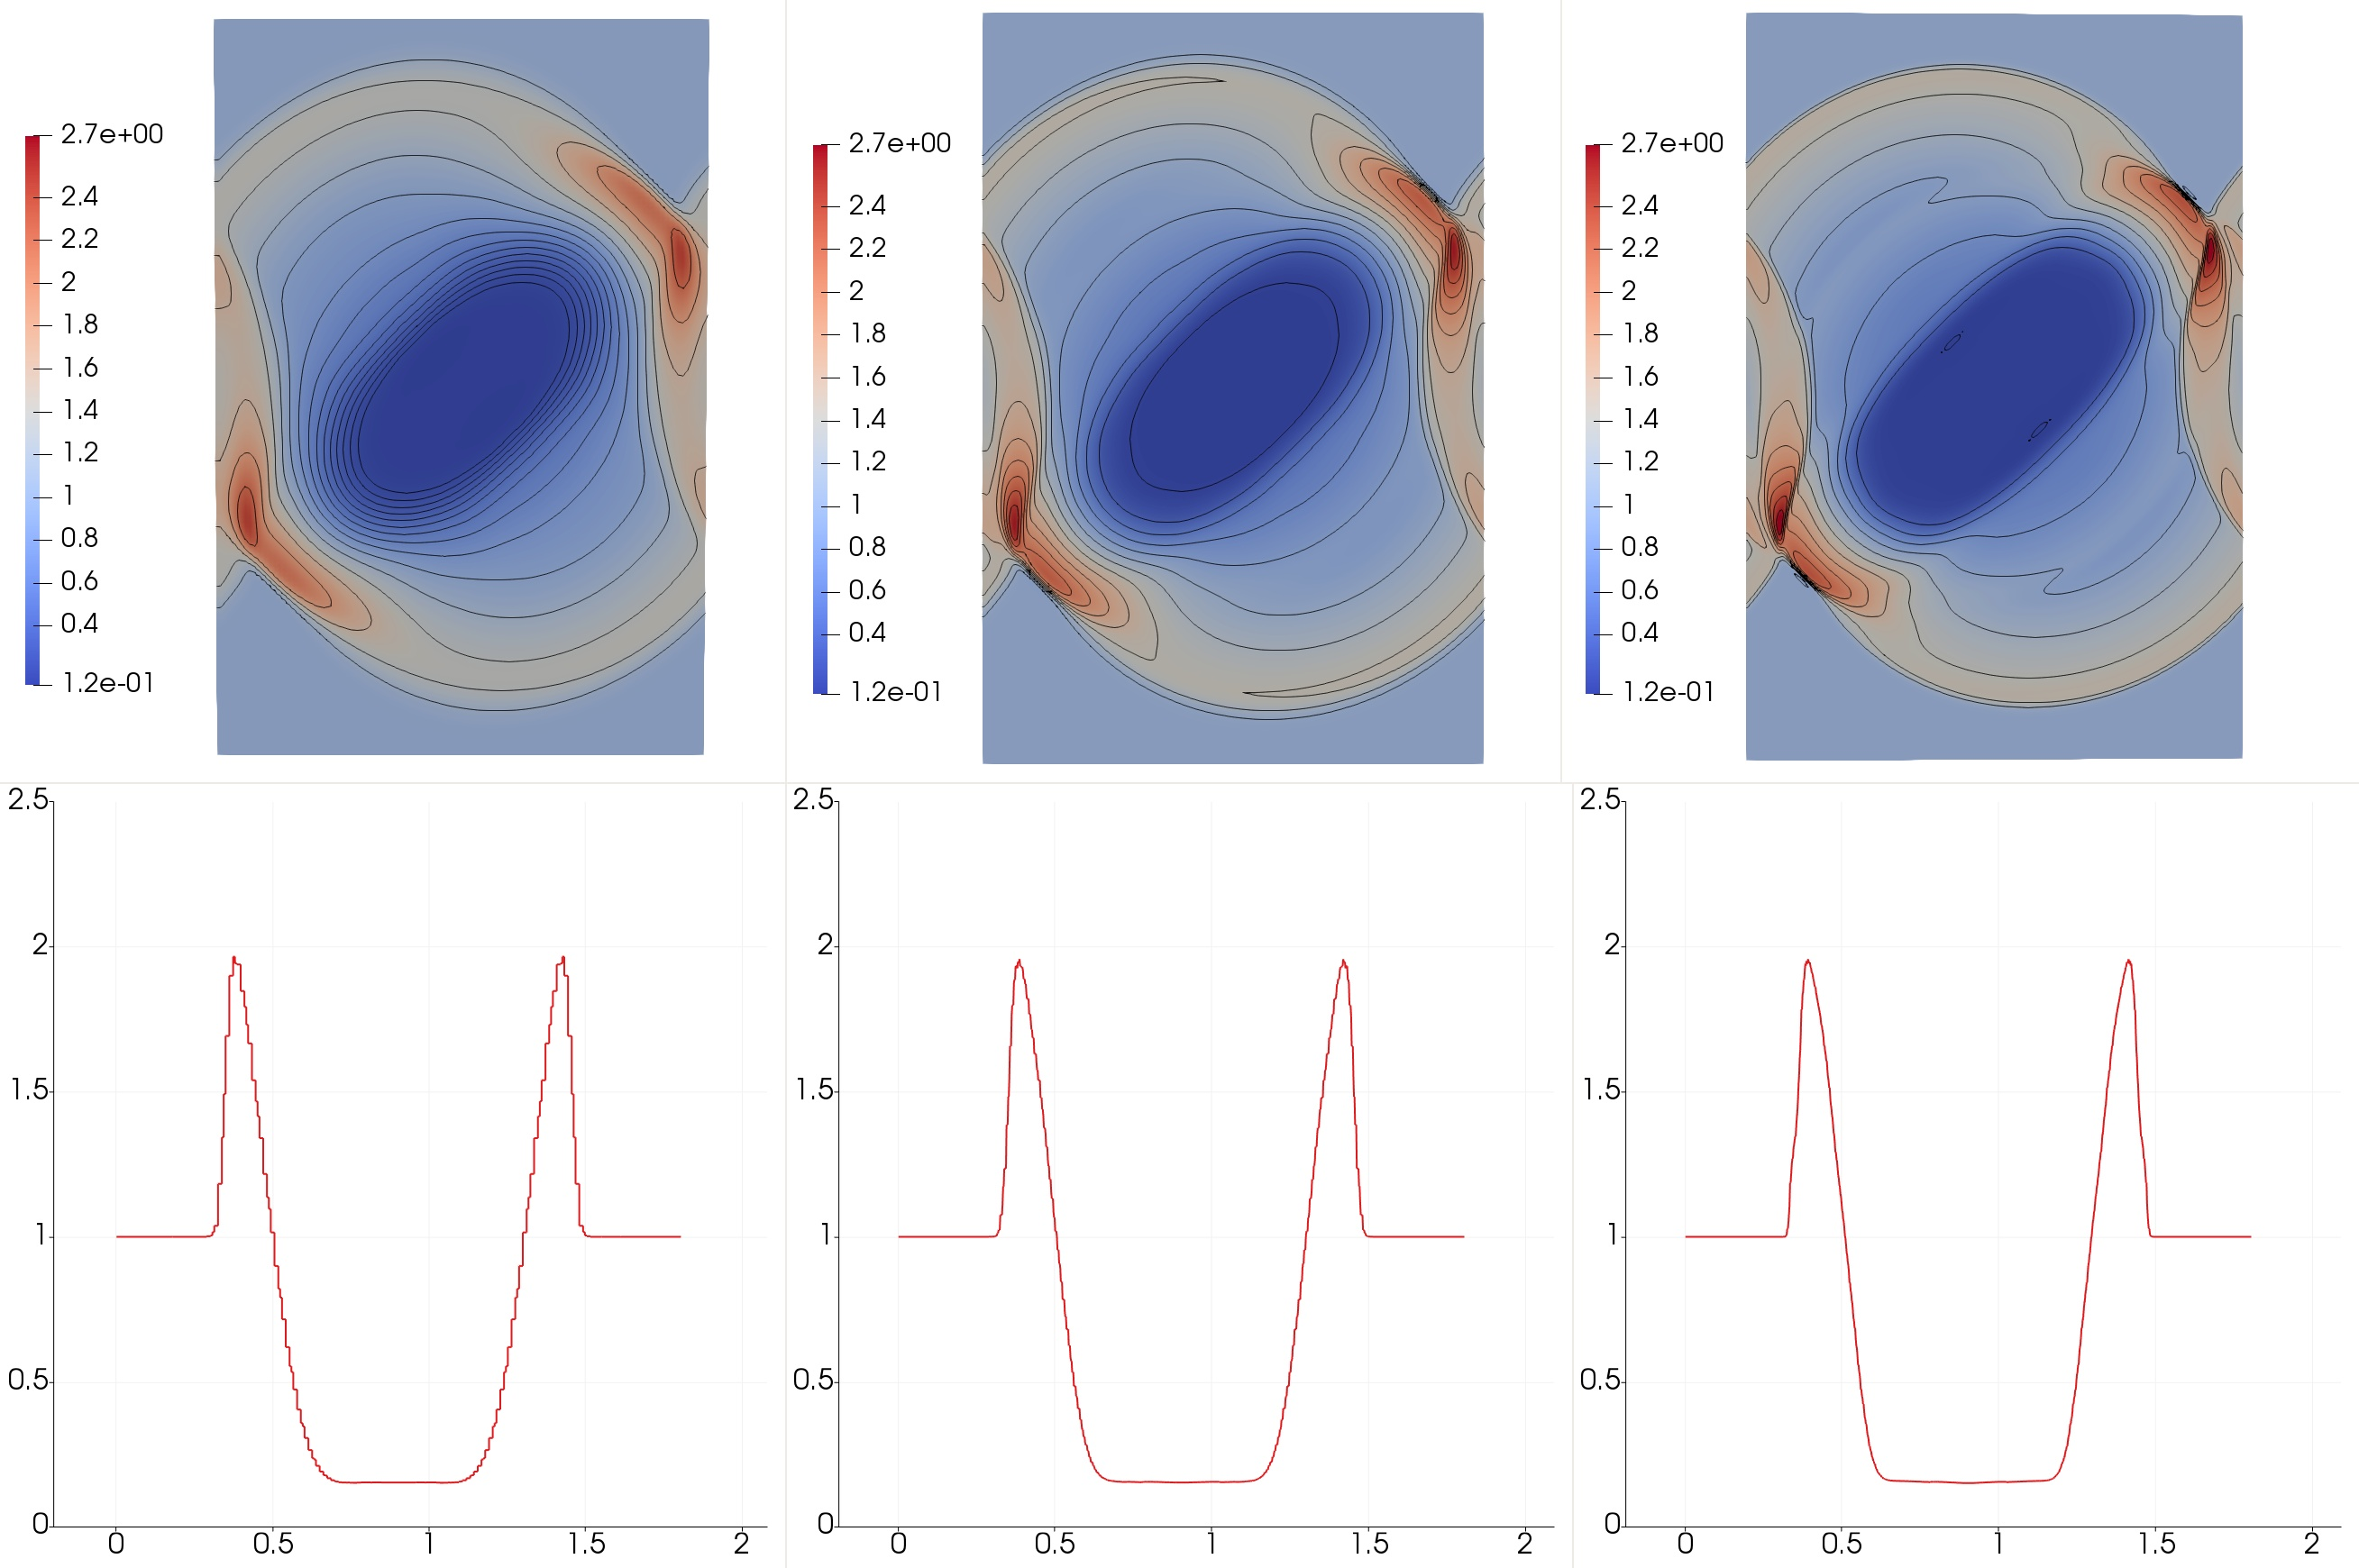
\includegraphics[width=0.95\textwidth]{img/mhd-blast/new/blast,noadapt5.jpg}
	\caption{Obtained results, $t \approx 0.3$, distribution of $\rho$ (top), with line distribution along bottom-left $\rightarrow$ top-right diagonal (bottom)}
	\label{figure:blastNew03}
	\end{center}
\end{figure}
\vspace{-8mm}

\begin{figure}[H]
	\begin{center}
		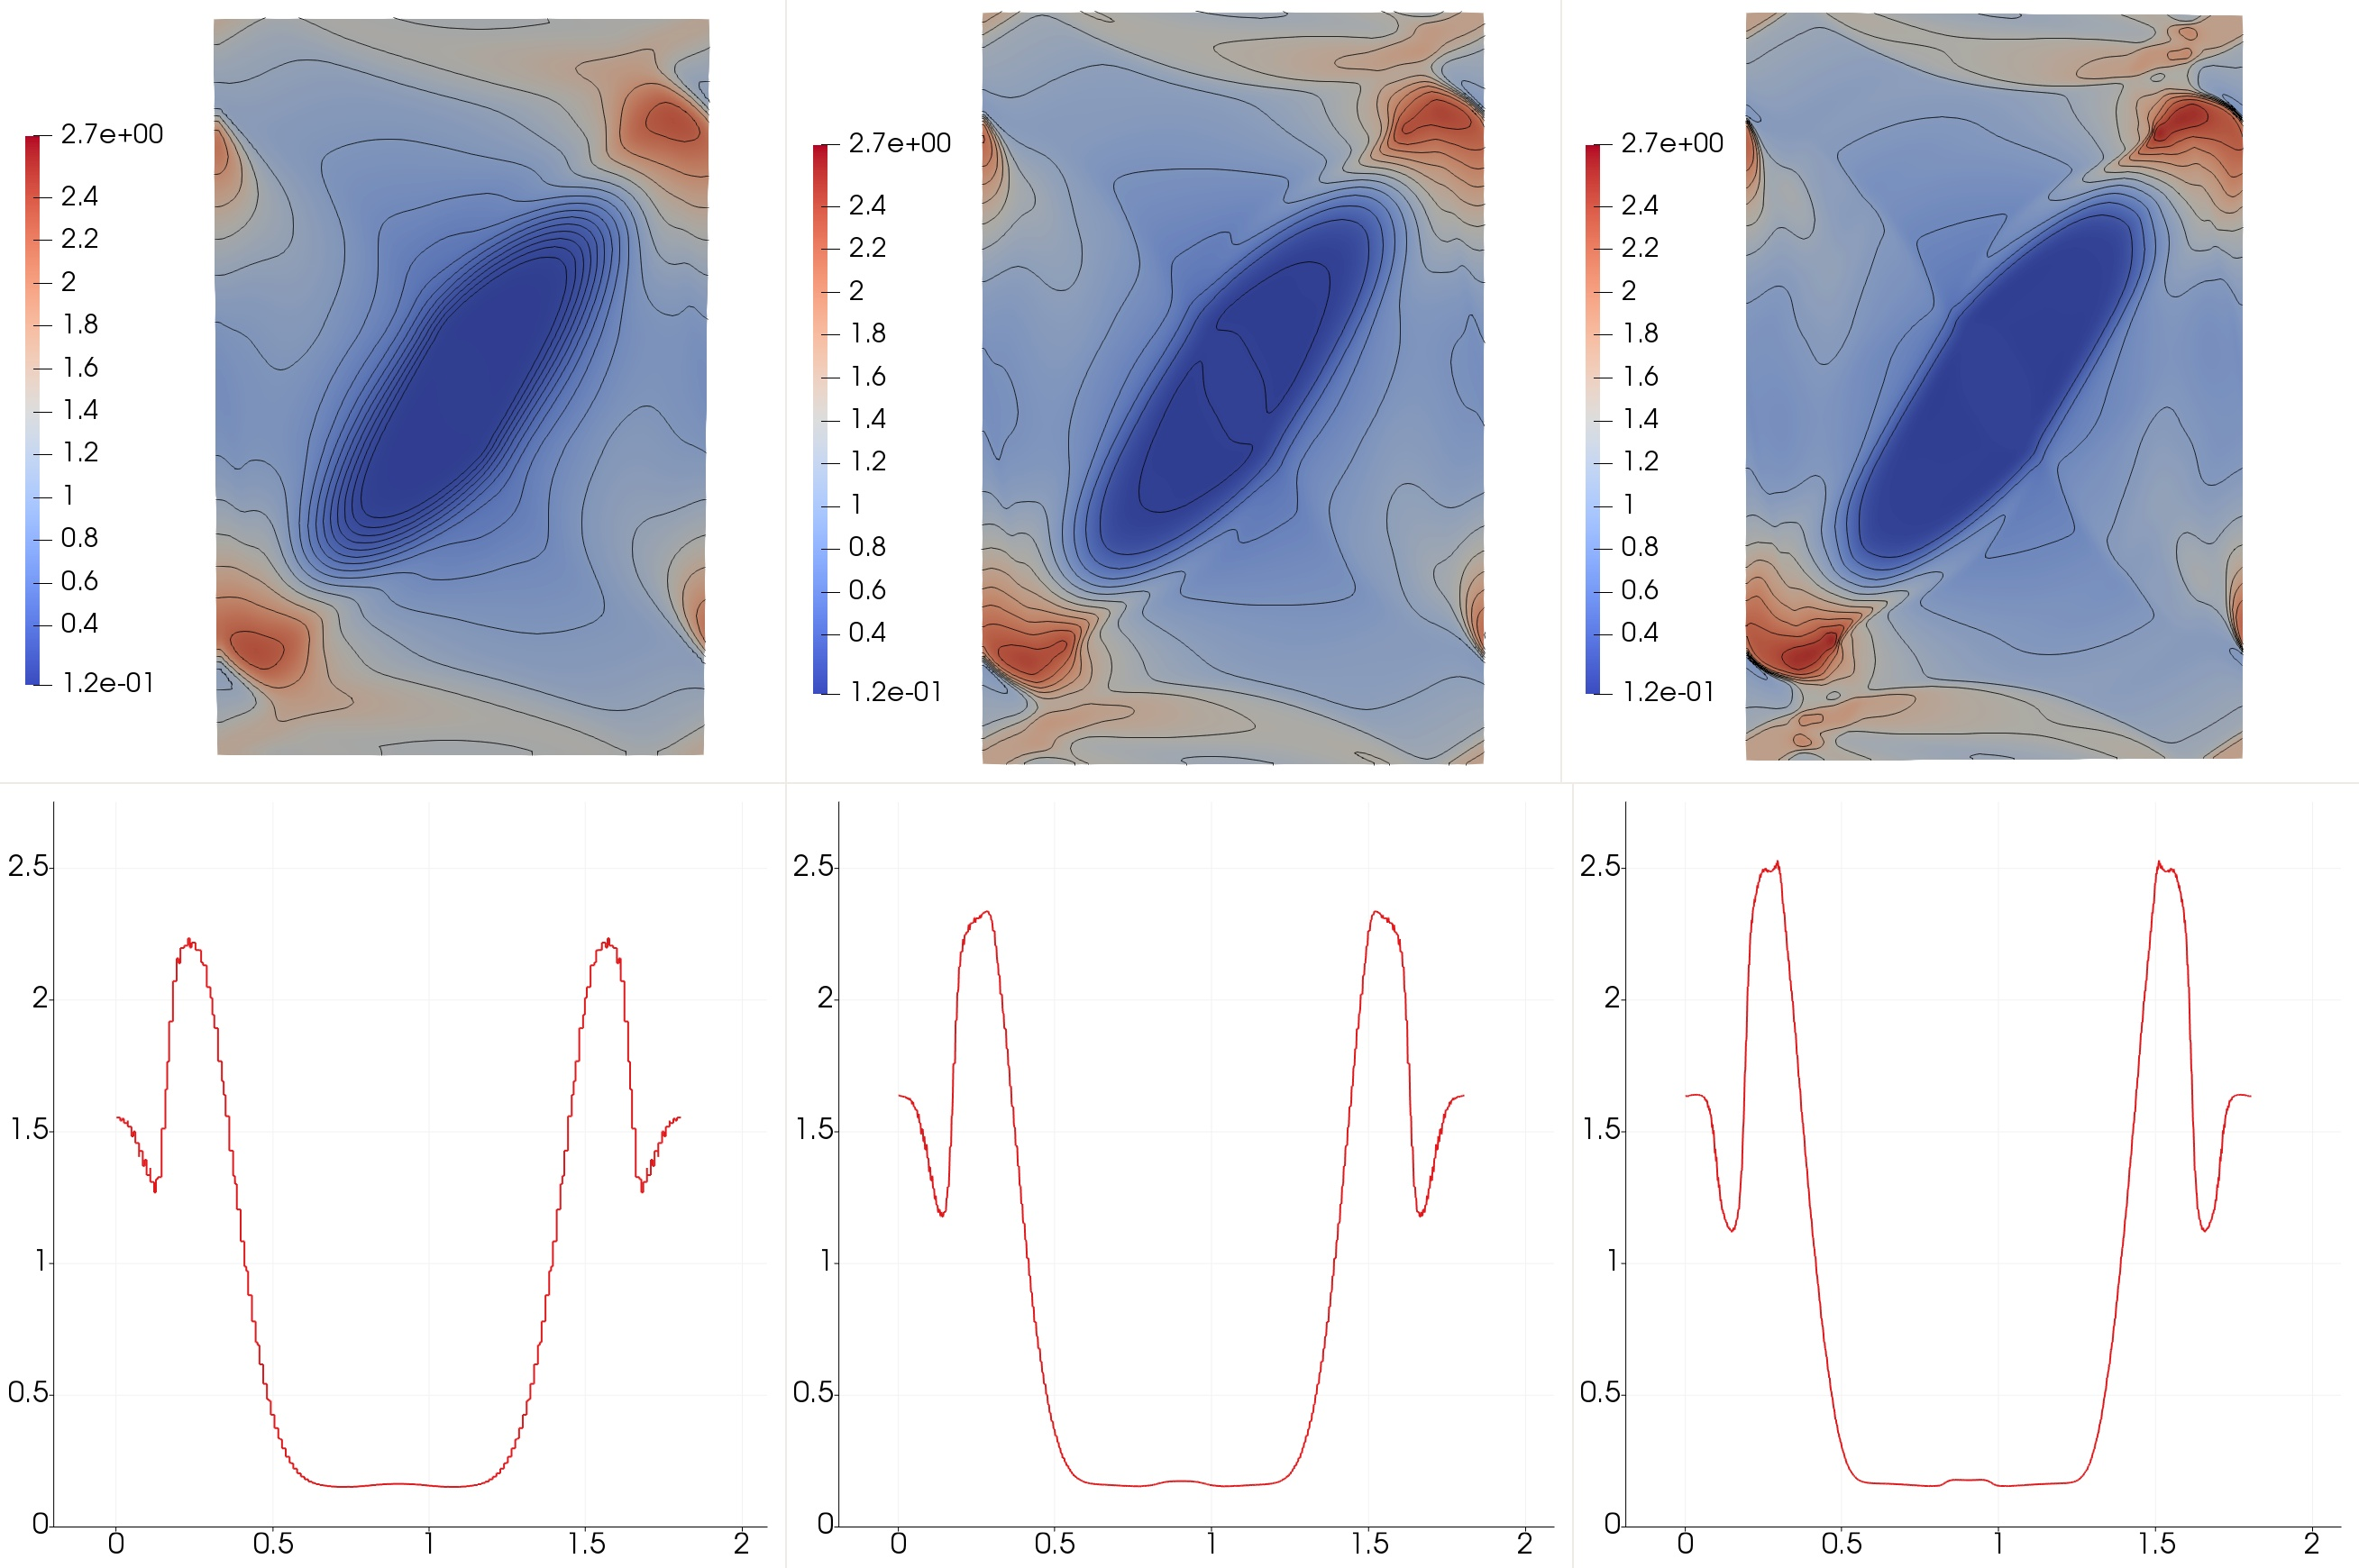
\includegraphics[width=0.95\textwidth]{img/mhd-blast/new/blast,noadapt9.jpg}
	\caption{Obtained results, $t \approx 0.45$, distribution of $\rho$ (top), with line distribution along bottom-left $\rightarrow$ top-right diagonal (bottom)}
	\label{figure:blastNew04}
	\end{center}
\end{figure}
\vspace{-8mm}

\begin{figure}[H]
	\begin{center}
		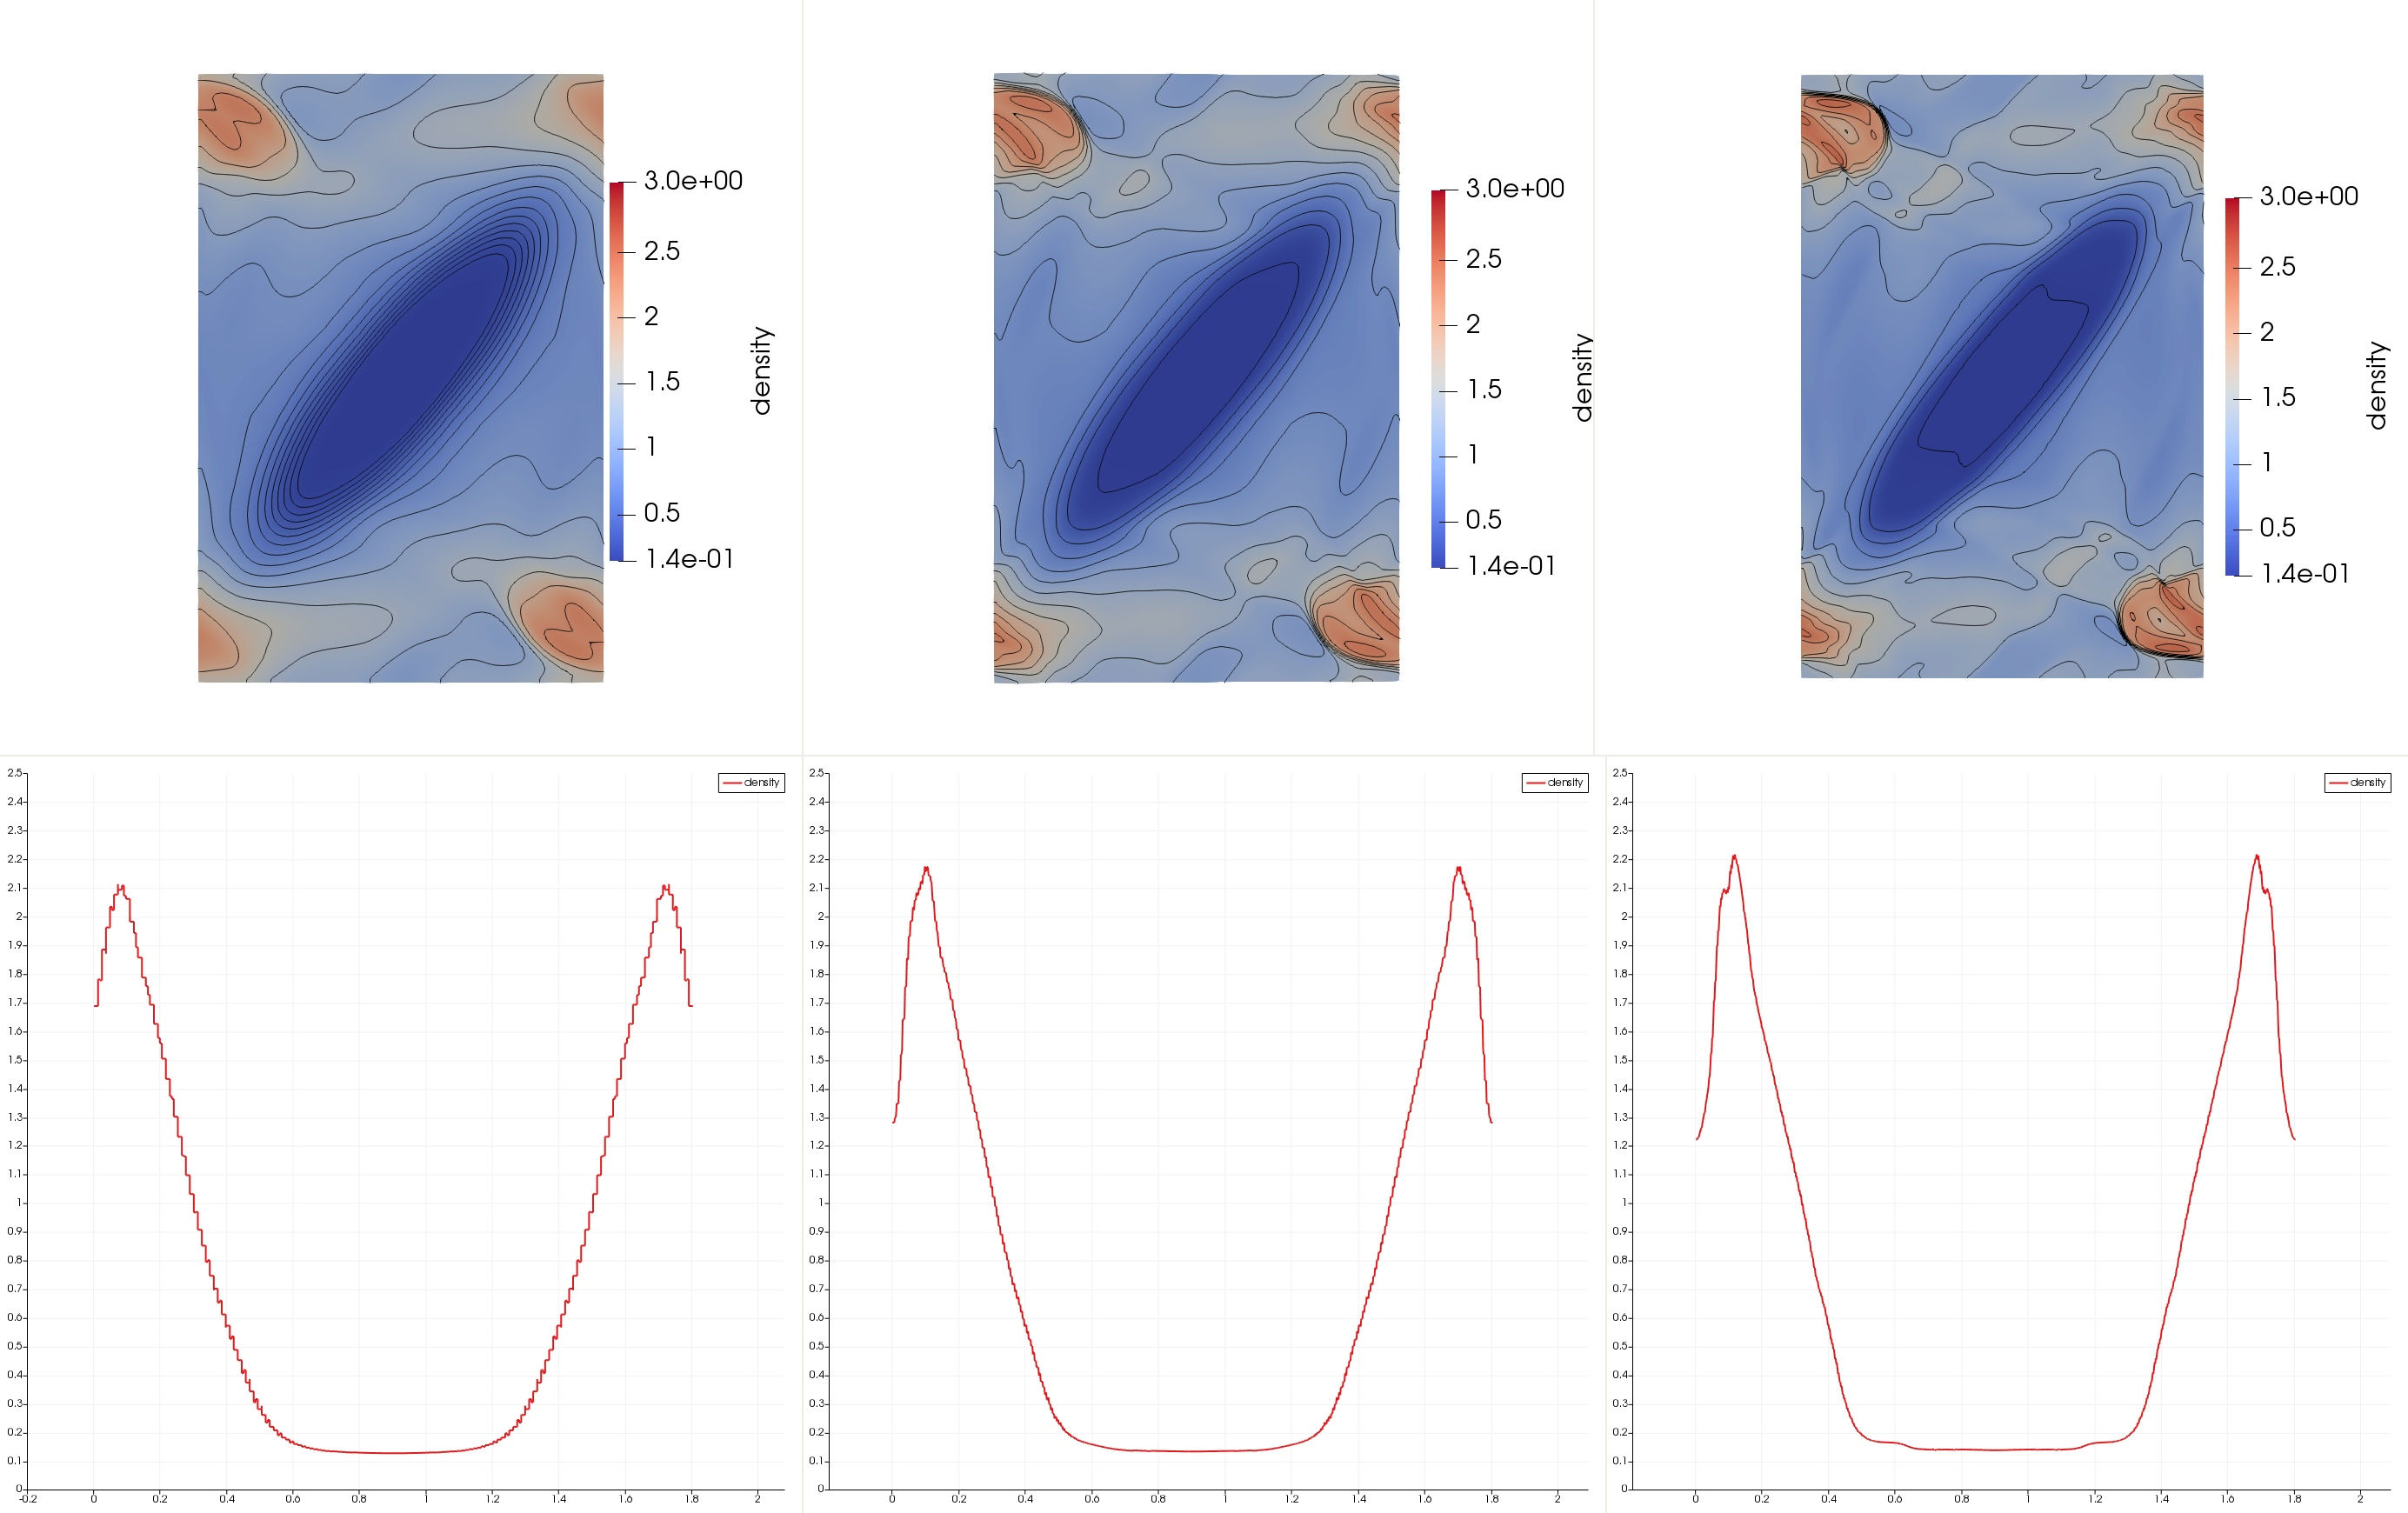
\includegraphics[width=0.95\textwidth]{img/mhd-blast/new/blast,noadapt14.jpg}
	\caption{Obtained results, $t = \approx 0.75$, distribution of $\rho$ (top), with line distribution along bottom-left $\rightarrow$ top-right diagonal (bottom)}
	\label{figure:blastNew05}
	\end{center}
\end{figure}
\vspace{-8mm}

\begin{figure}[H]
	\begin{center}
		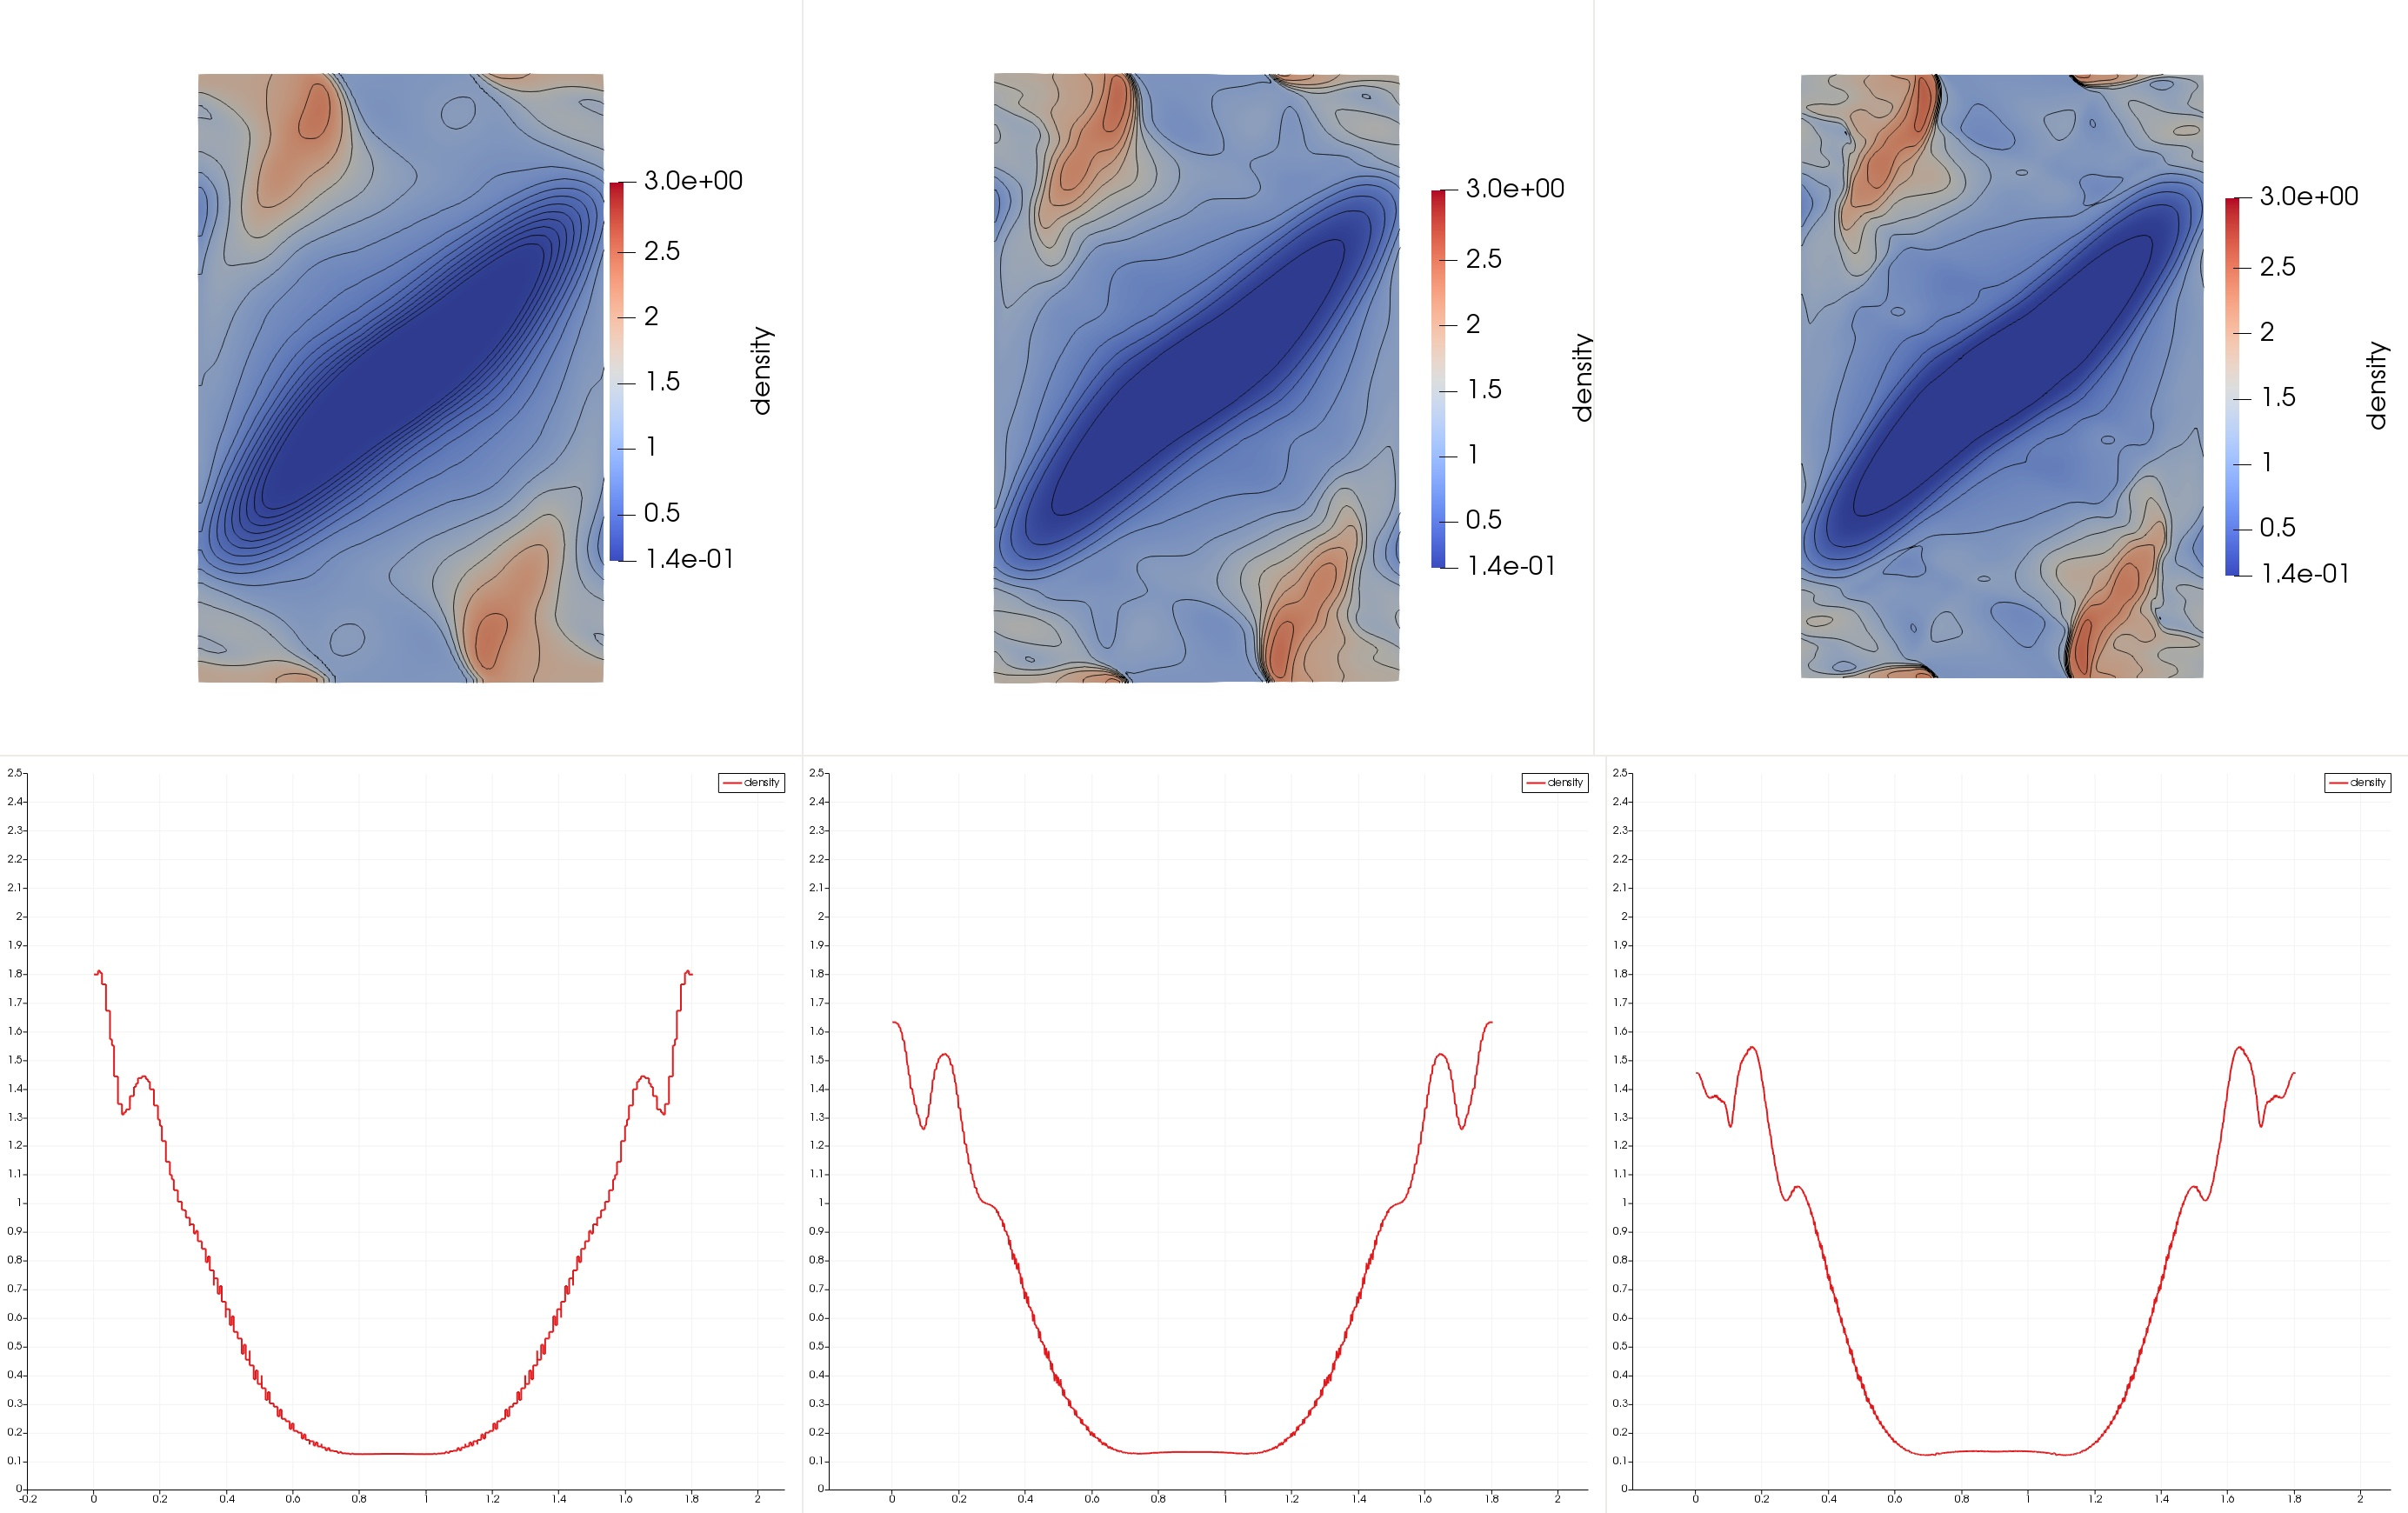
\includegraphics[width=0.95\textwidth]{img/mhd-blast/new/blast,noadapt18.jpg}
	\caption{Obtained results, $t \approx 0.95$, distribution of $\rho$ (top), with line distribution along bottom-left $\rightarrow$ top-right diagonal (bottom)}
	\label{figure:blastNew06}
	\end{center}
\end{figure}
\vspace{-8mm}

It is clearly visible, that the solution is somehow smeared, and the uniform mesh refinements improve the situation, but not greatly, and for a large cost of storage size for storing much more mesh elements.
\paragraph{}
In order to amend the situation, and be able to obtain a higher-quality solution with a reasonable number of mesh elements, piecewise-linear basis functions need to be used. Results with piecewise-linear basis functions, on three successively uniformly refined meshes are given in \crefrange{figure:blastNew11}{figure:blastNew16}. The meshes for these computations contained:
\begin{itemize}
\item $50 \times 75$ elements (left)
\item $100 \times 150$ elements (middle)
\item $200 \times 300$ elements (right)
\end{itemize}

\begin{figure}[H]
	\begin{center}
		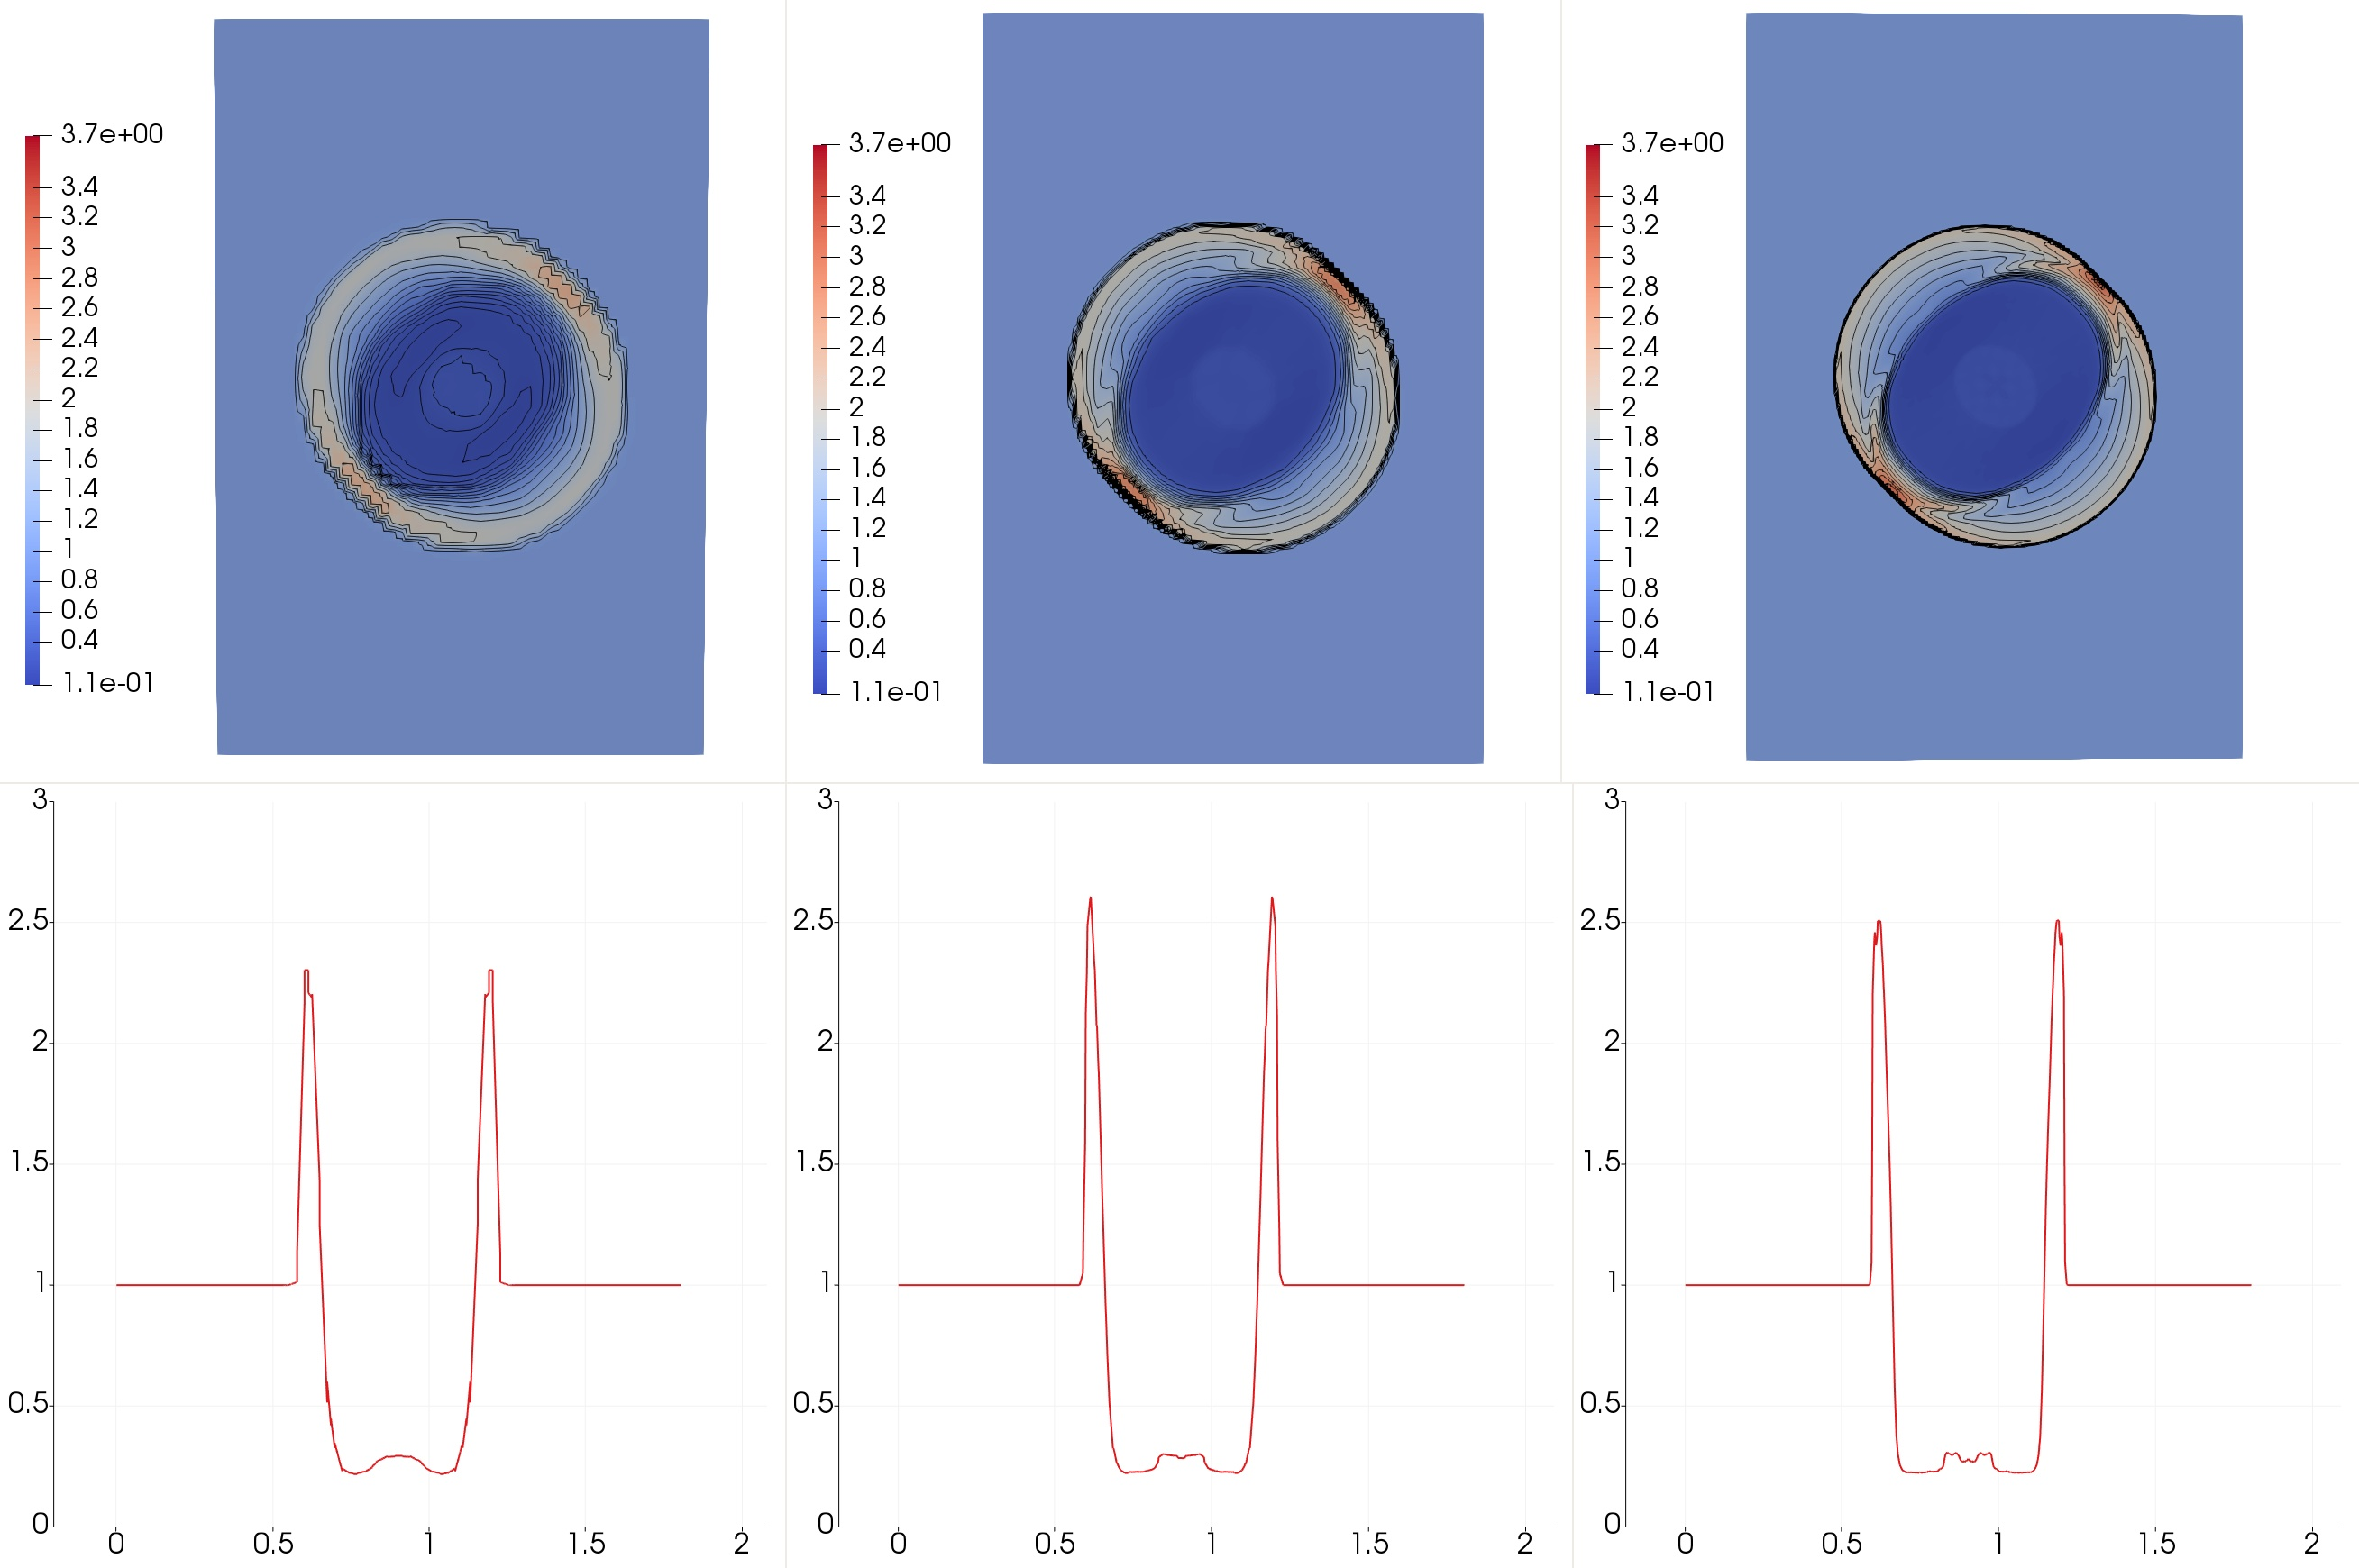
\includegraphics[width=0.92\textwidth]{img/mhd-blast/new/blast,1noadapt1.jpg}
	\caption{Obtained results, $t \approx 0.1$, distribution of $\rho$ (top), with line distribution along bottom-left $\rightarrow$ top-right diagonal (bottom)}
	\label{figure:blastNew11}
	\end{center}
\end{figure}
\vspace{-8mm}

\begin{figure}[H]
	\begin{center}
		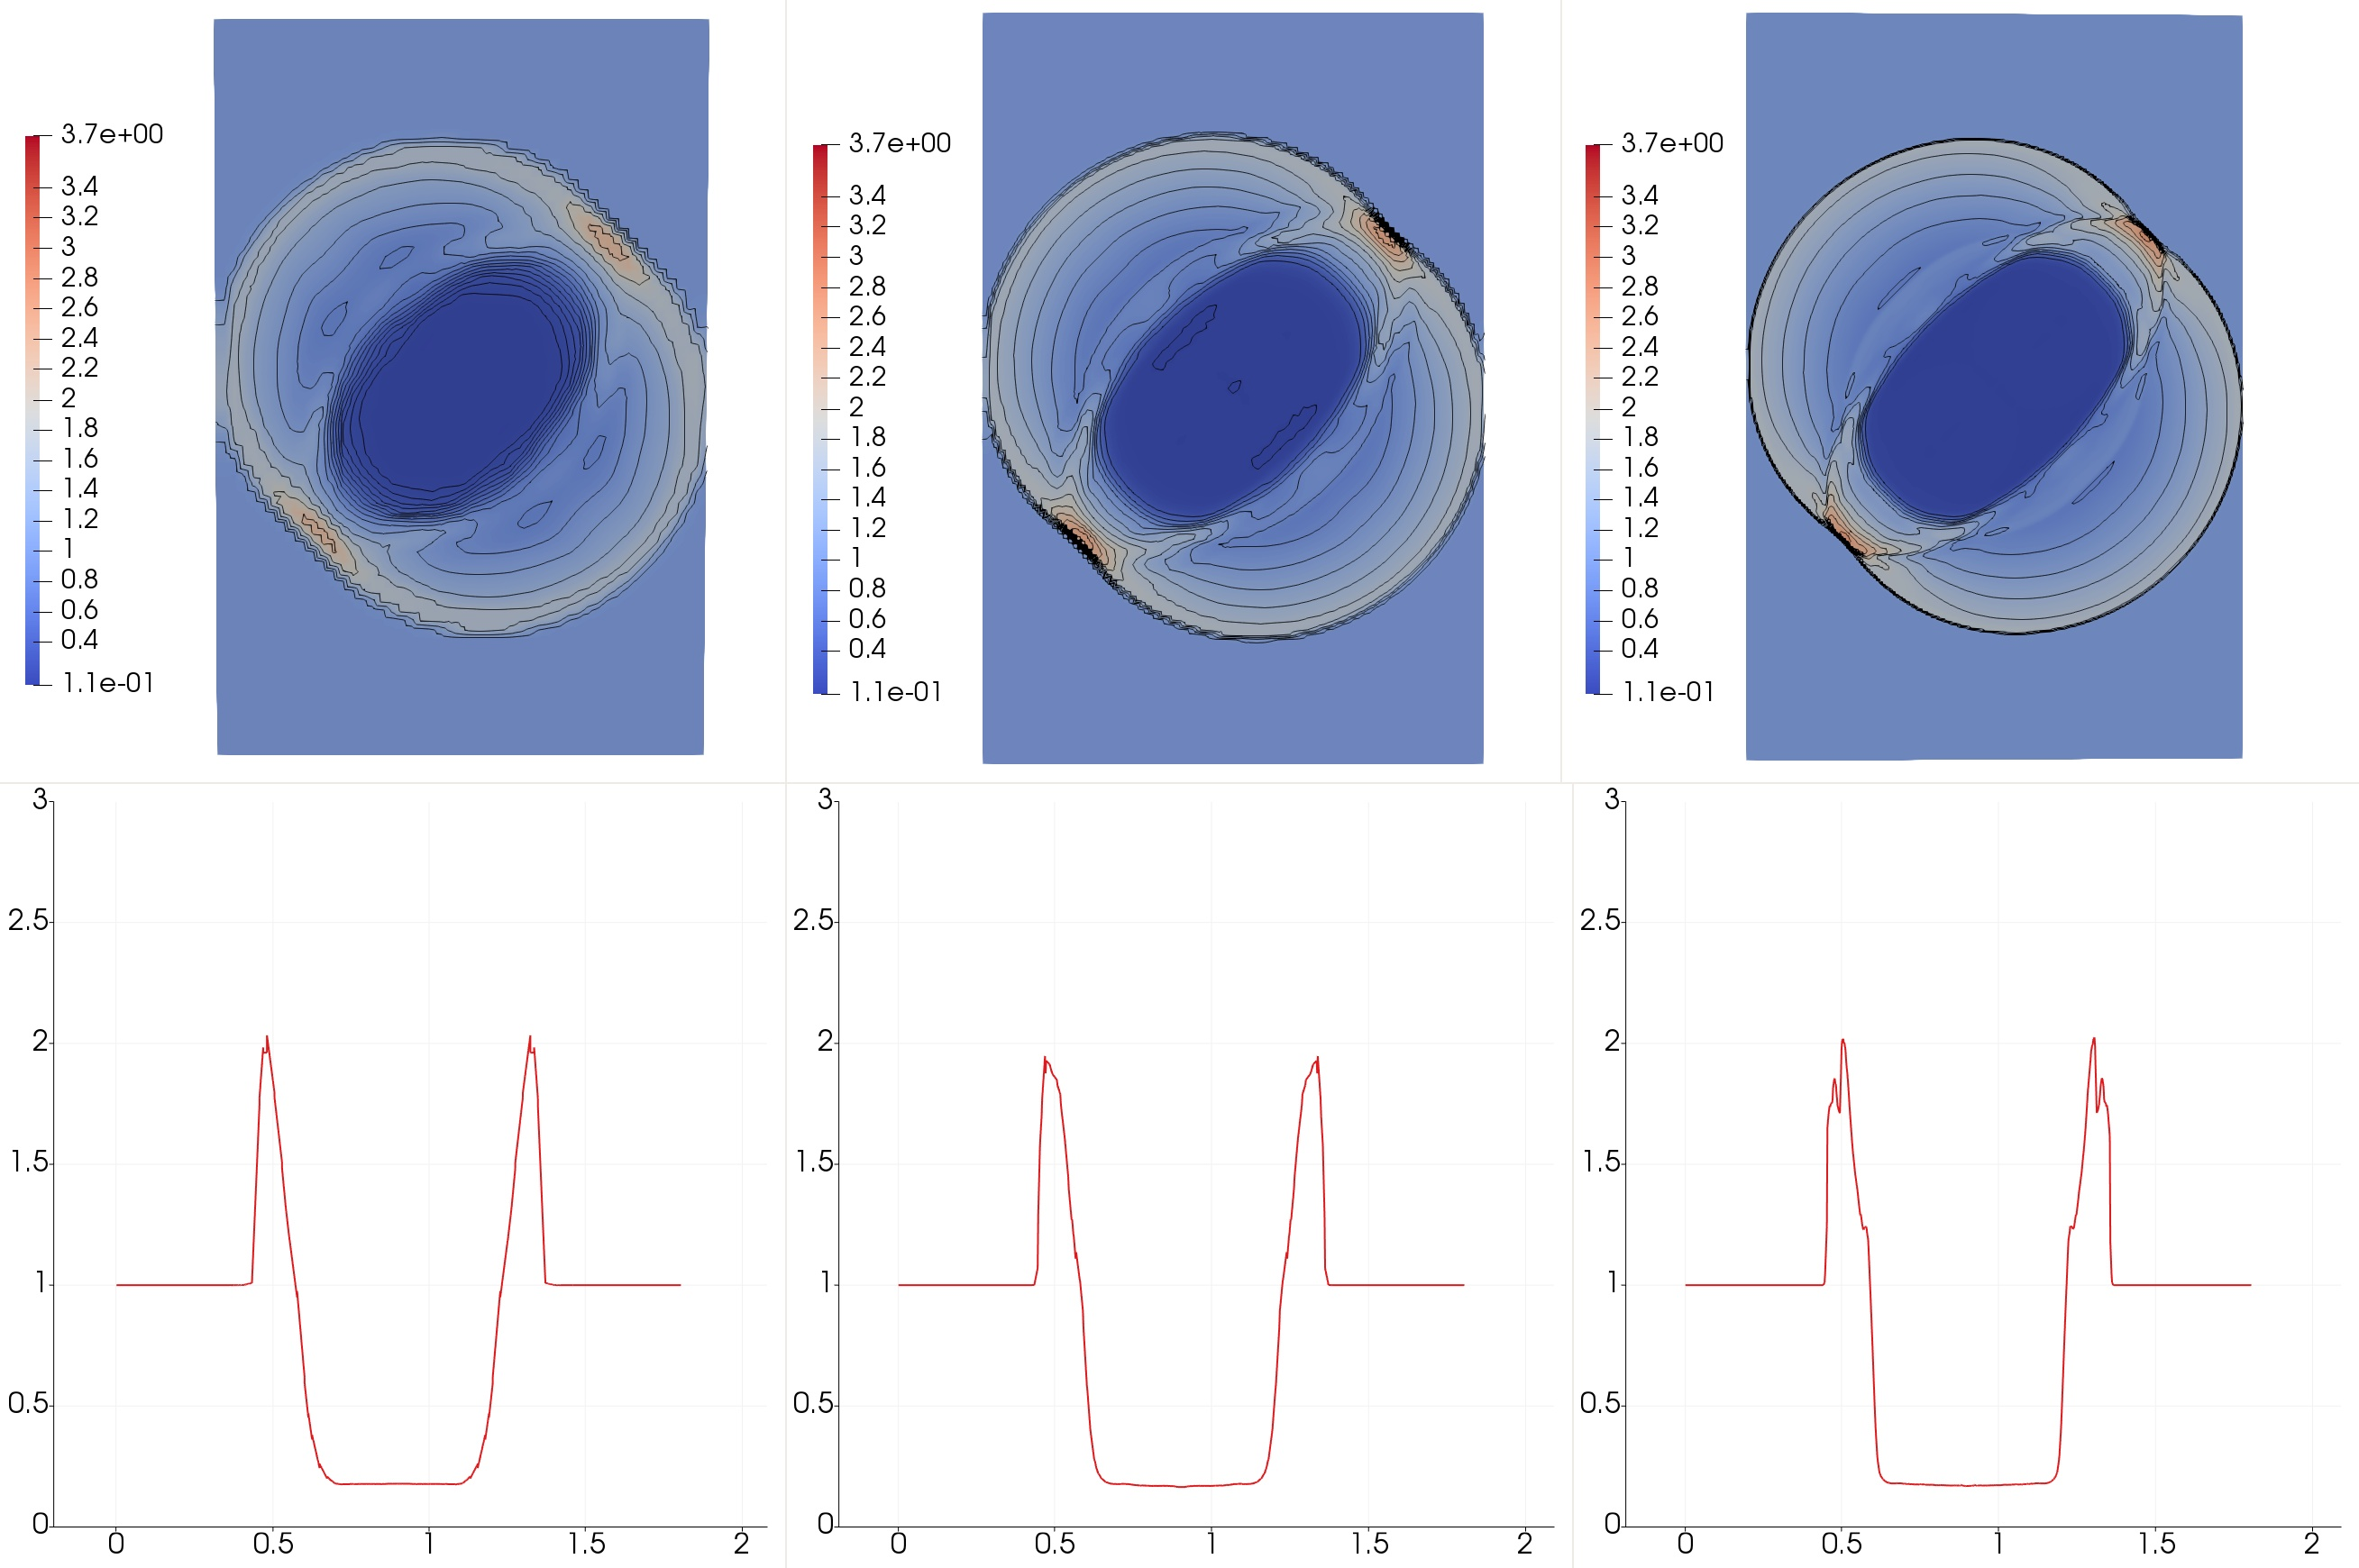
\includegraphics[width=0.92\textwidth]{img/mhd-blast/new/blast,1noadapt3.jpg}
	\caption{Obtained results, $t = \approx 0.2$, distribution of $\rho$ (top), with line distribution along bottom-left $\rightarrow$ top-right diagonal (bottom)}
	\label{figure:blastNew12}
	\end{center}
\end{figure}
\vspace{-8mm}

\begin{figure}[H]
	\begin{center}
		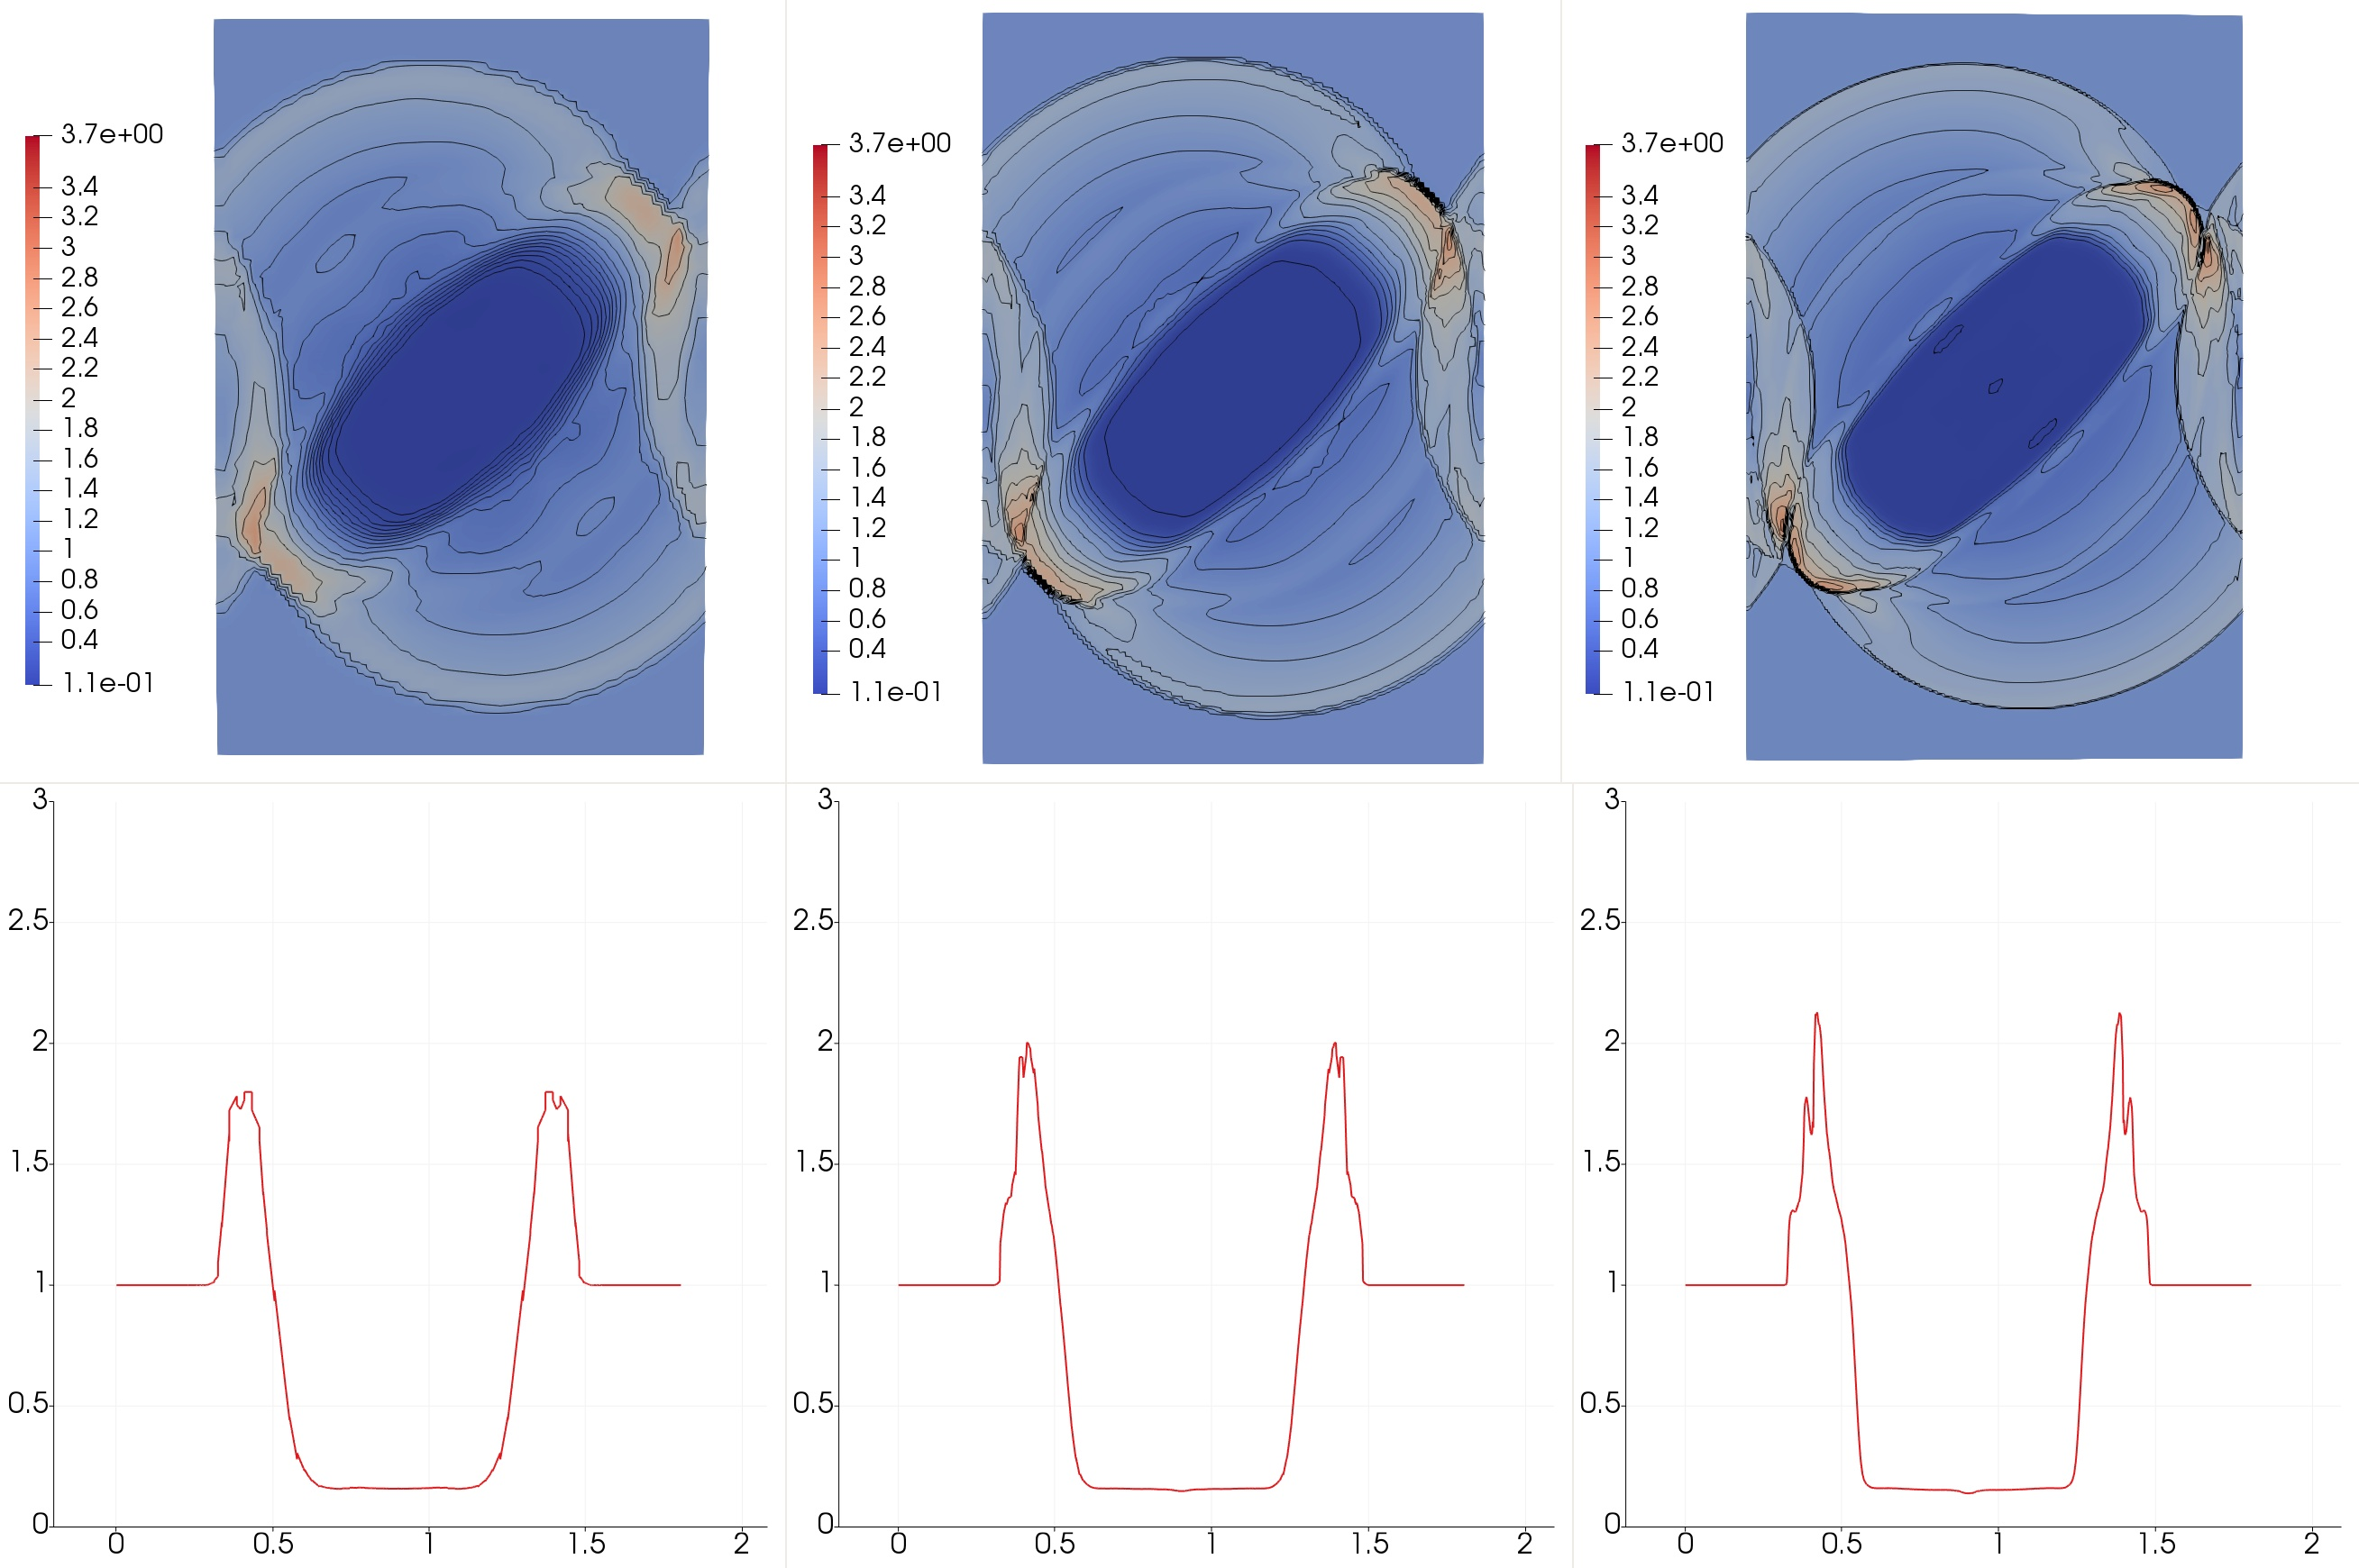
\includegraphics[width=0.92\textwidth]{img/mhd-blast/new/blast,1noadapt5.jpg}
	\caption{Obtained results, $t \approx 0.3$, distribution of $\rho$ (top), with line distribution along bottom-left $\rightarrow$ top-right diagonal (bottom)}
	\label{figure:blastNew13}
	\end{center}
\end{figure}
\vspace{-8mm}

\begin{figure}[H]
	\begin{center}
		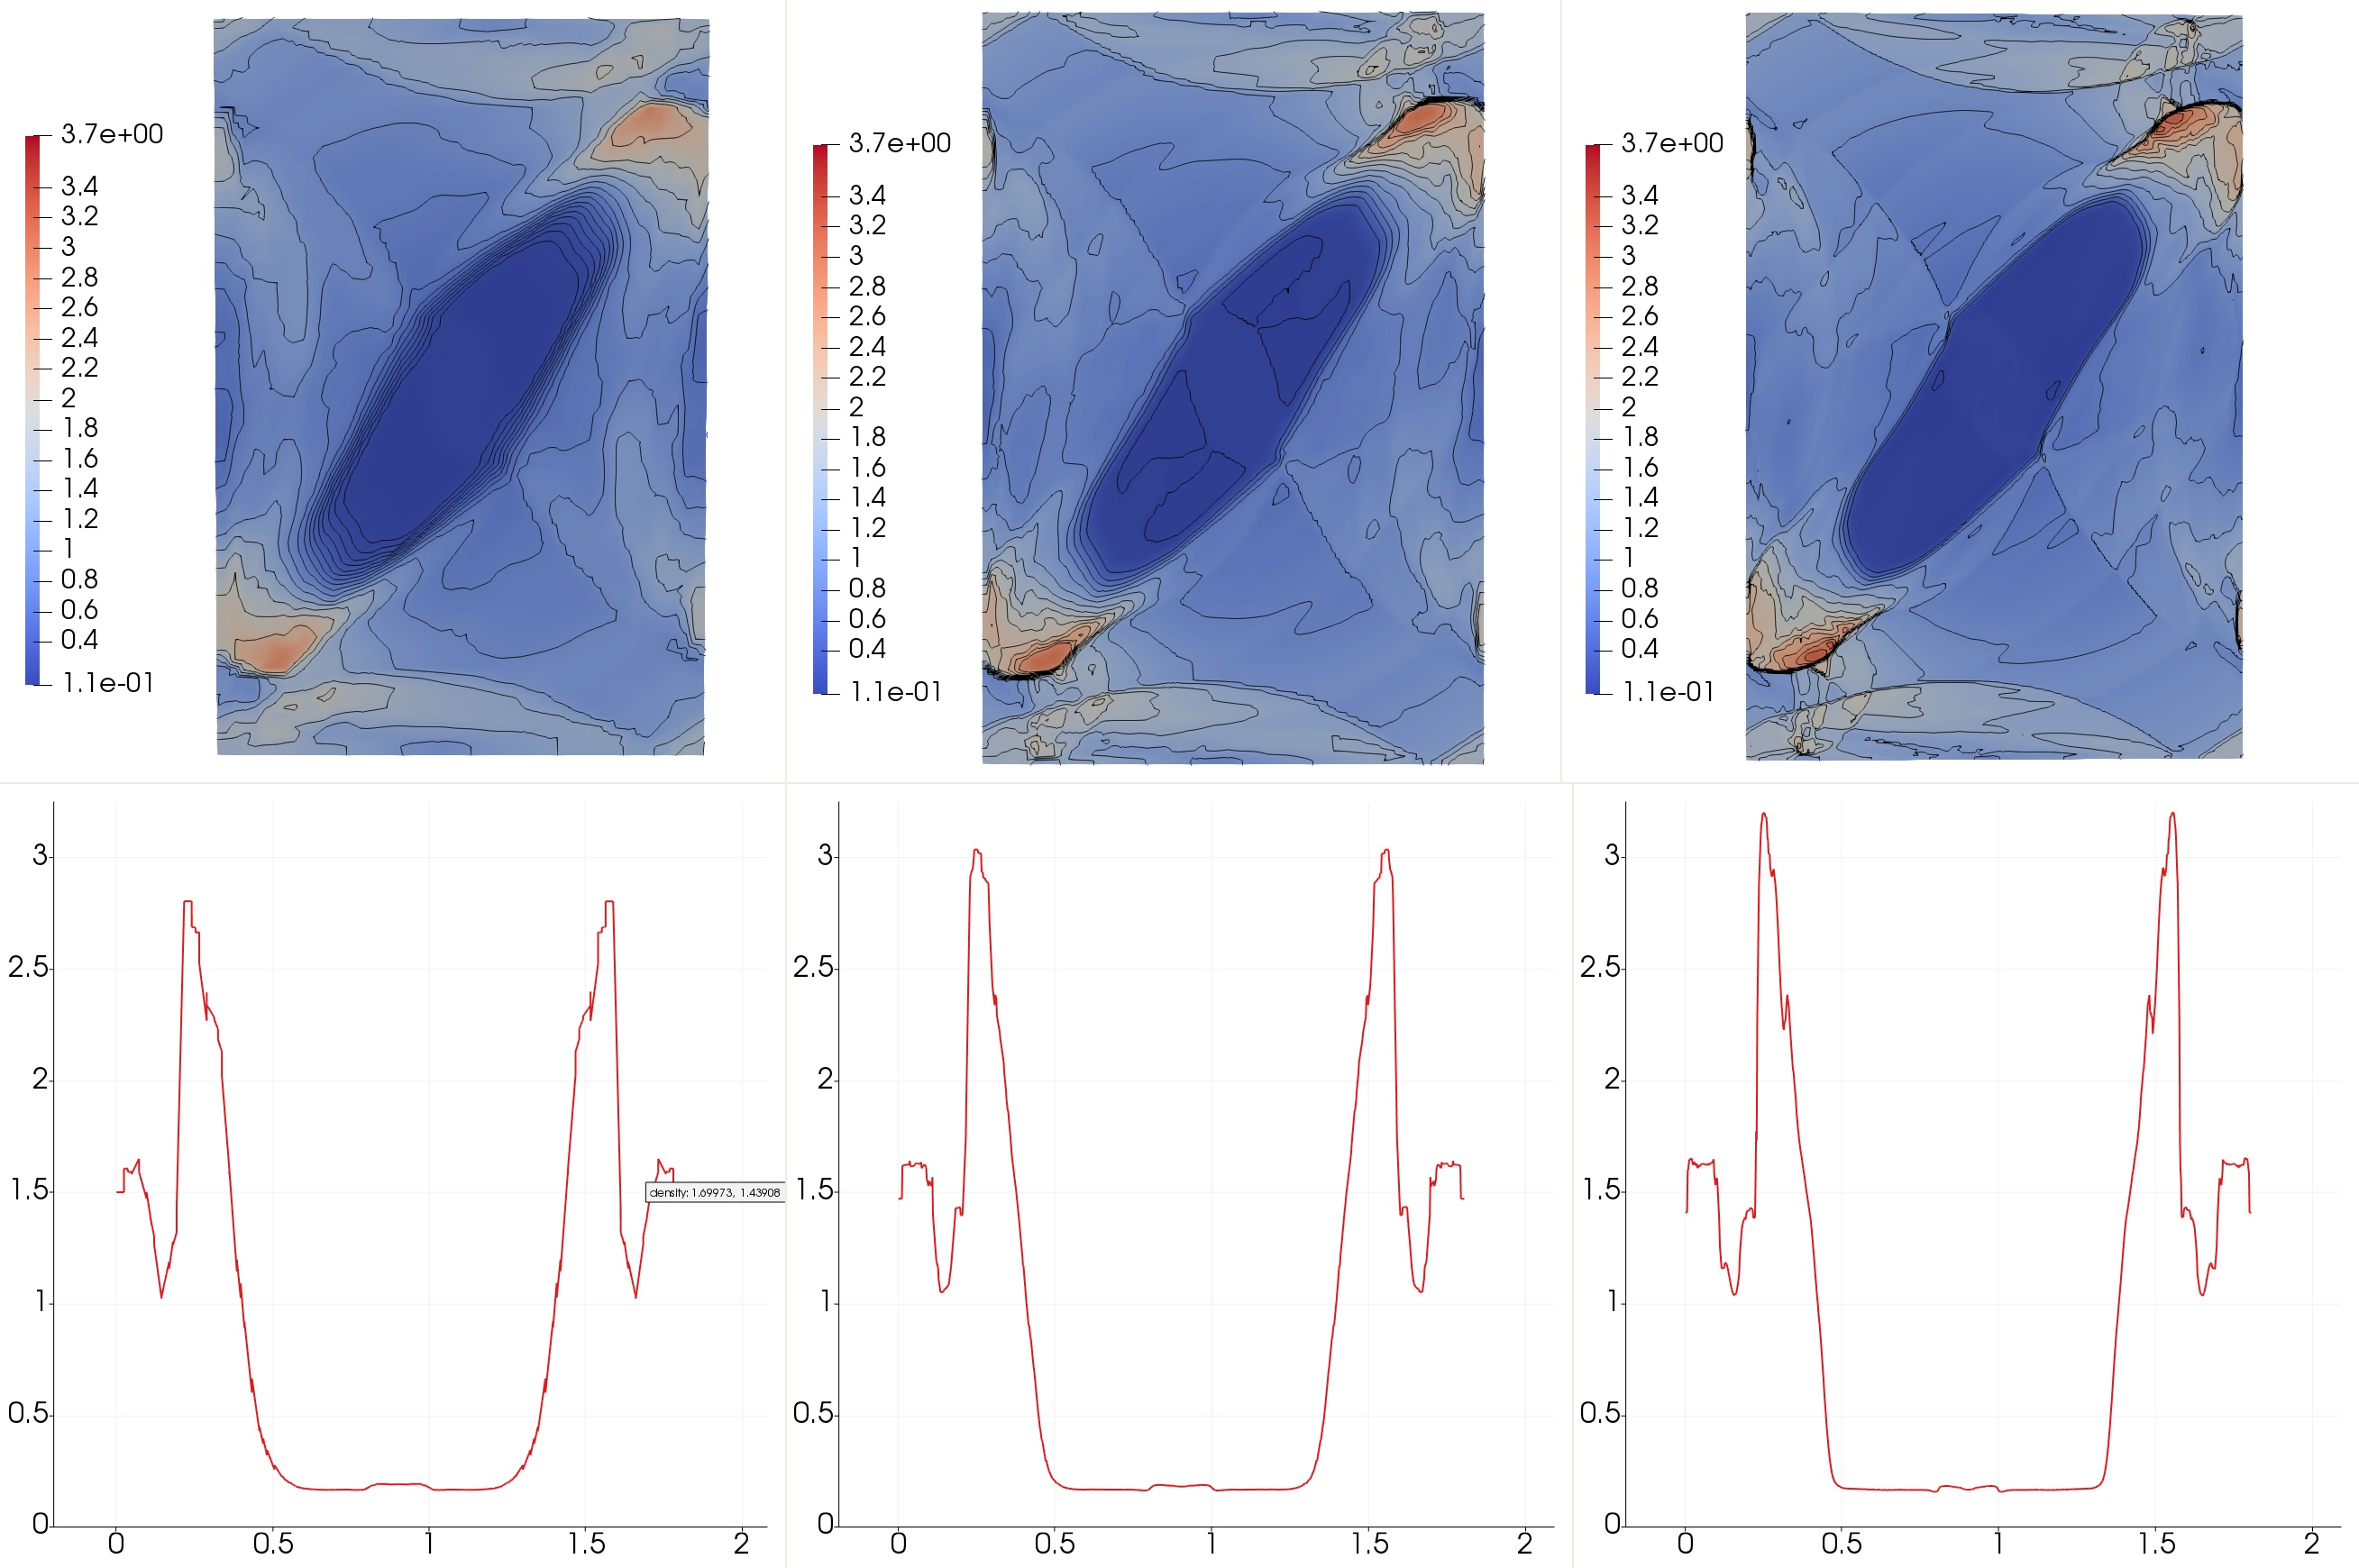
\includegraphics[width=0.92\textwidth]{img/mhd-blast/new/blast,1noadapt9.jpg}
	\caption{Obtained results, $t \approx 0.45$, distribution of $\rho$ (top), with line distribution along bottom-left $\rightarrow$ top-right diagonal (bottom)}
	\label{figure:blastNew14}
	\end{center}
\end{figure}
\vspace{-8mm}

\begin{figure}[H]
	\begin{center}
		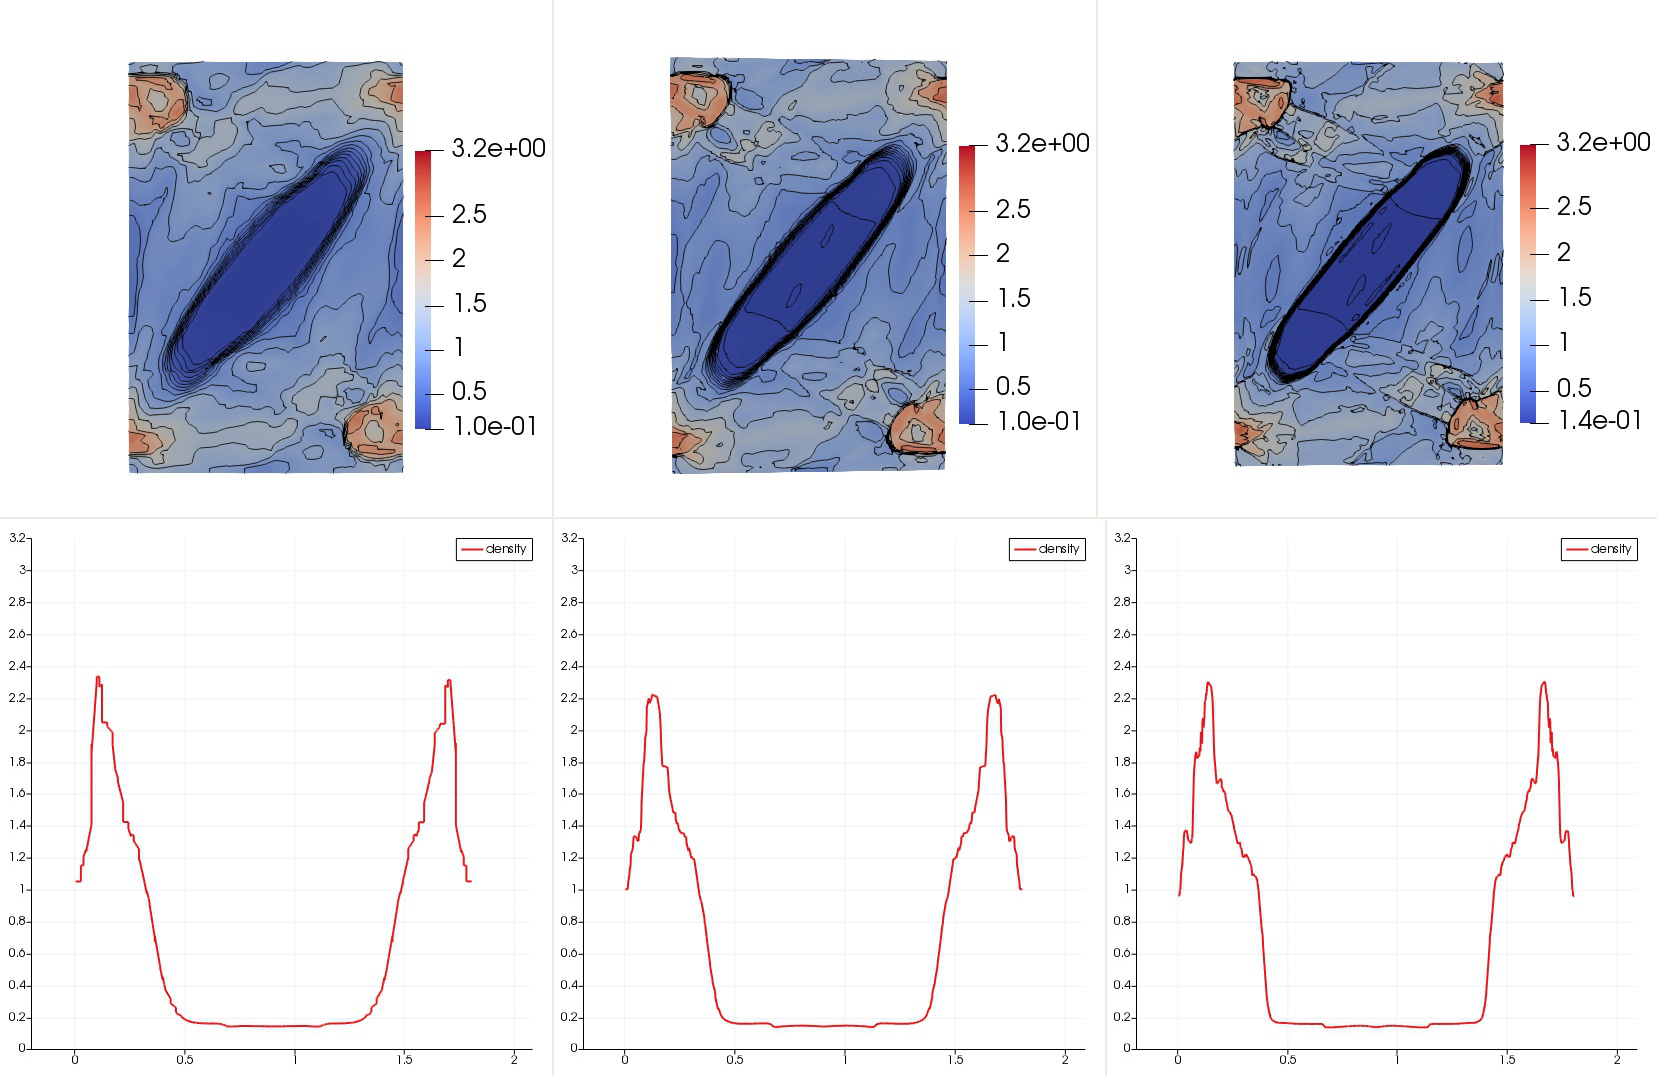
\includegraphics[width=0.92\textwidth]{img/mhd-blast/new/blast,1noadapt14.jpg}
	\caption{Obtained results, $t = \approx 0.75$, distribution of $\rho$ (top), with line distribution along bottom-left $\rightarrow$ top-right diagonal (bottom)}
	\label{figure:blastNew15}
	\end{center}
\end{figure}
\vspace{-8mm}

\begin{figure}[H]
	\begin{center}
		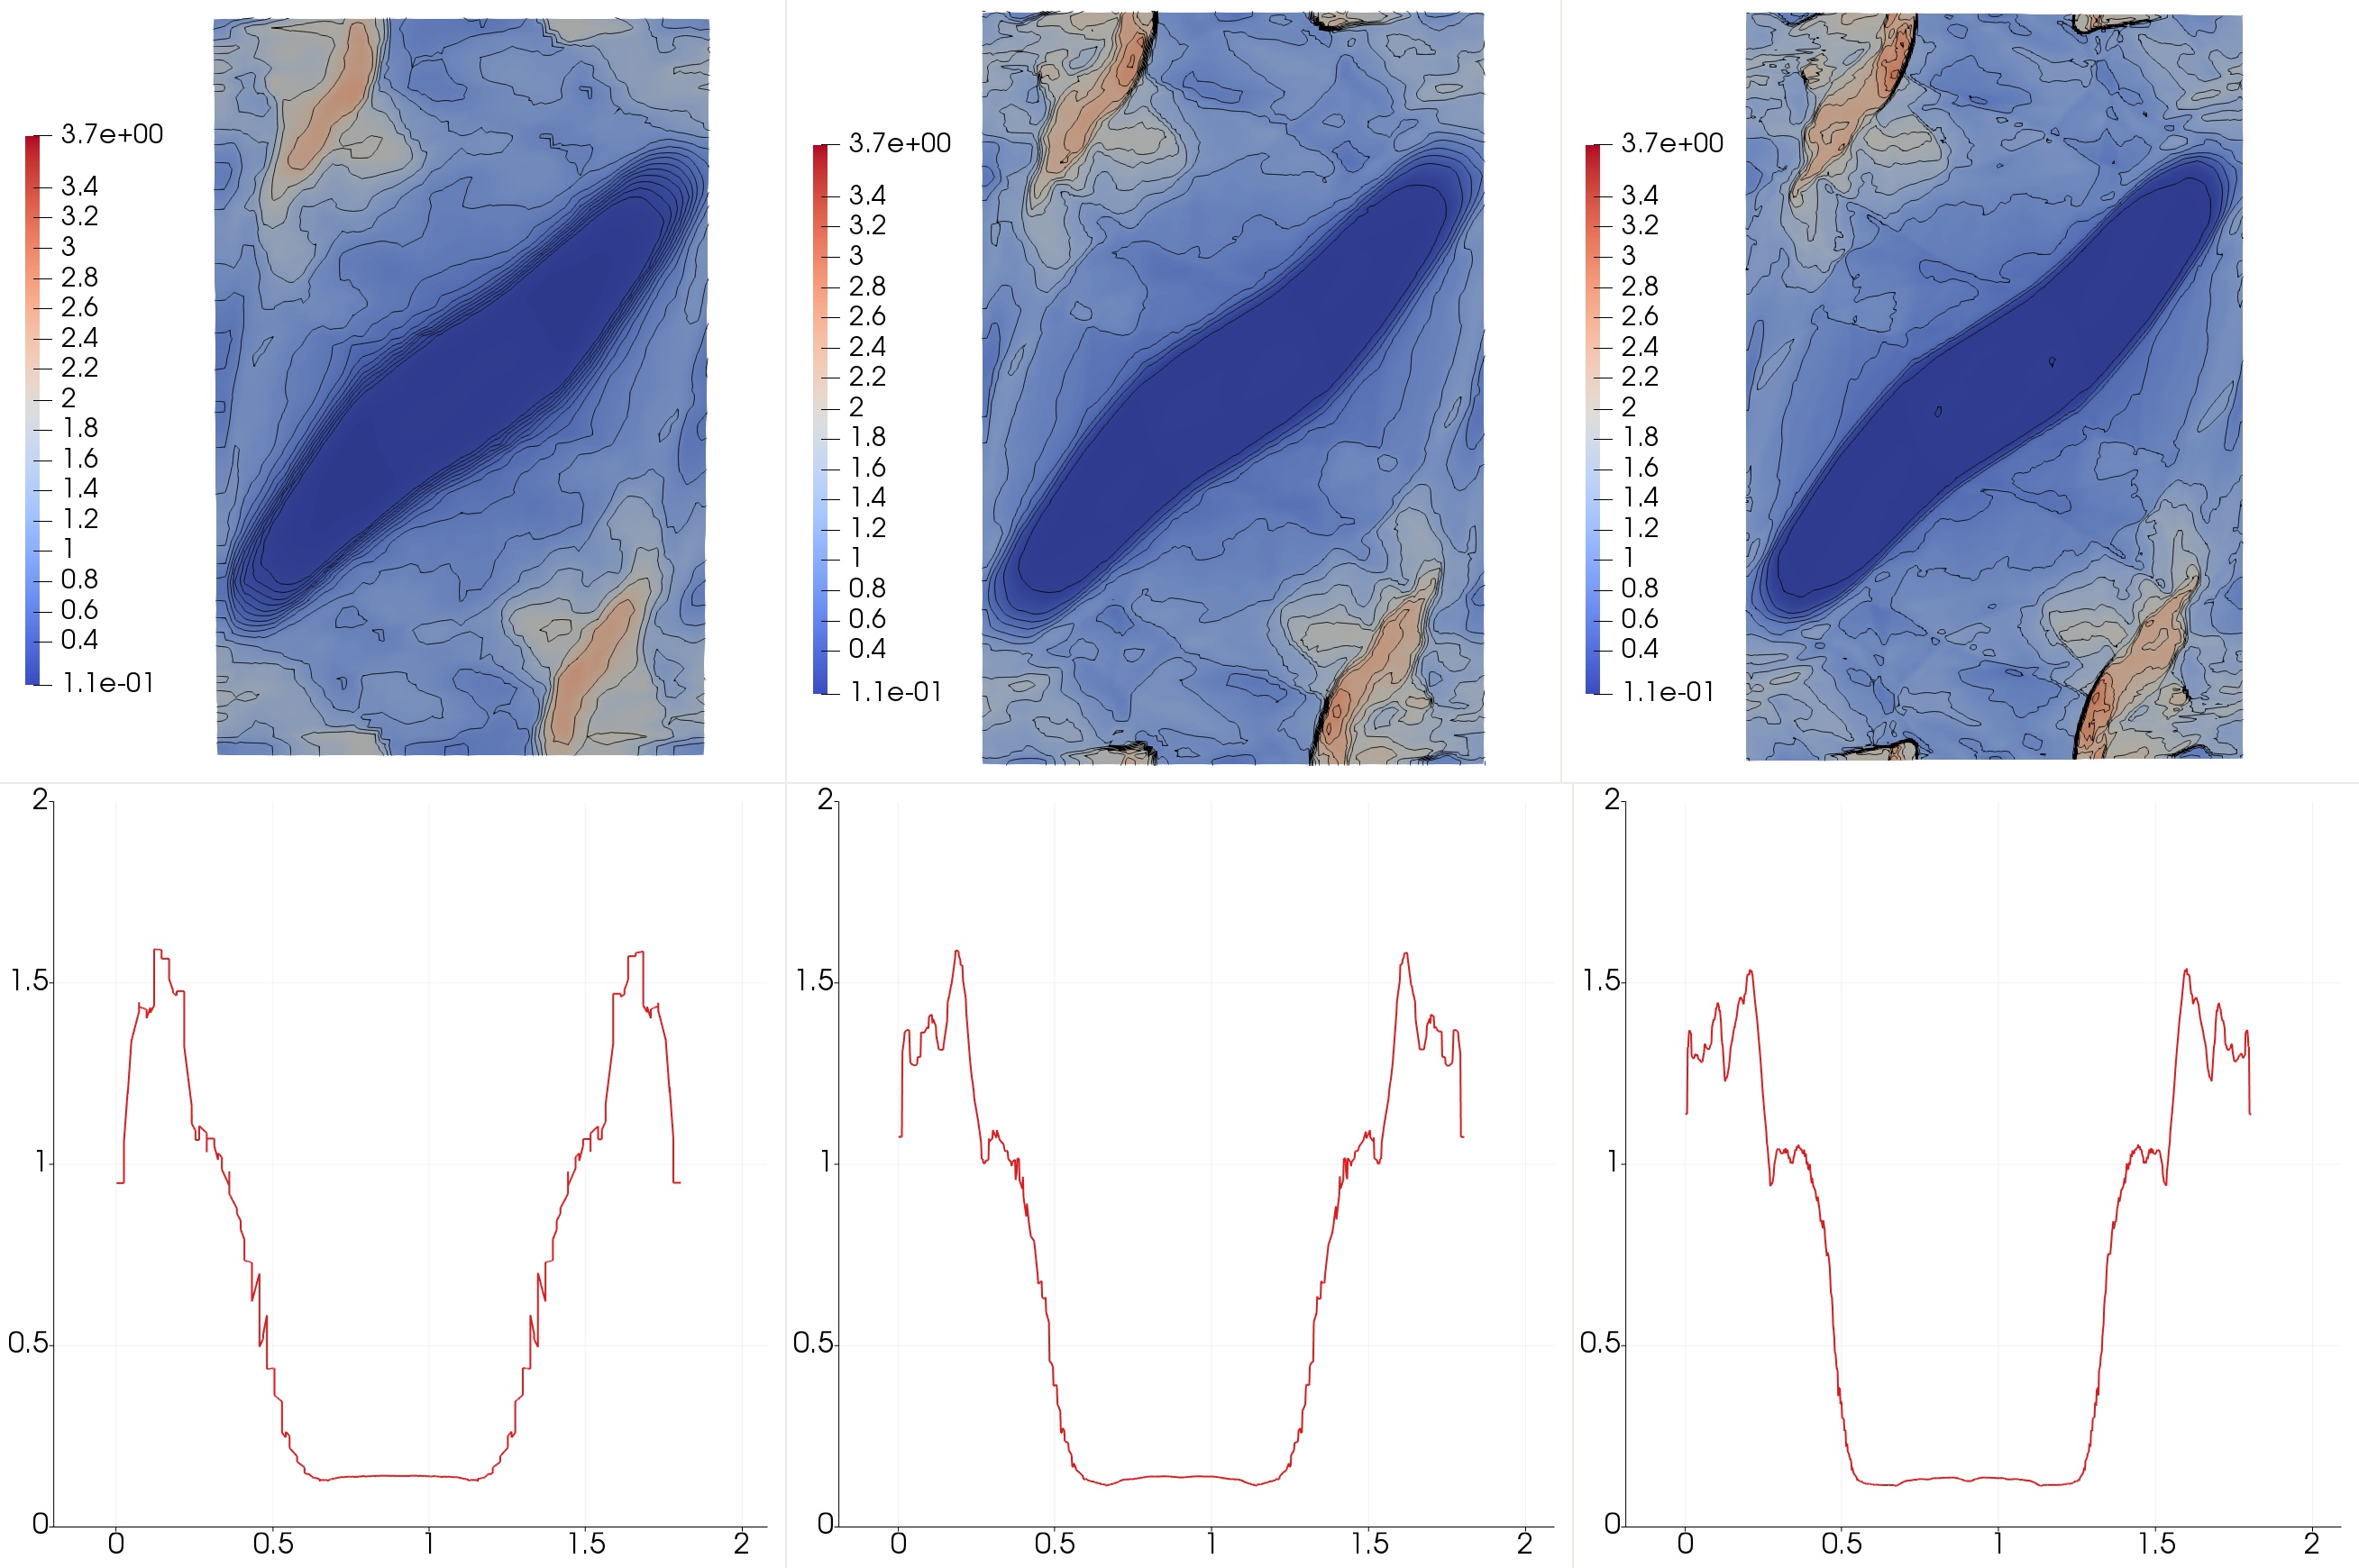
\includegraphics[width=0.92\textwidth]{img/mhd-blast/new/blast,1noadapt18.jpg}
	\caption{Obtained results, $t \approx 0.95$, distribution of $\rho$ (top), with line distribution along bottom-left $\rightarrow$ top-right diagonal (bottom)}
	\label{figure:blastNew16}
	\end{center}
\end{figure}
\vspace{-4mm}

Now, the solution with piecewise-linear functions is of much higher quality and the solution snapshots displayed in \cref{figure:blastFinal} are practically identical (and even more detailed) as the solution from \cite{blastNew1} in \cref{figure:blastRef}. Of course, this comes at a price of increased number of degrees of freedom, and associated increase in the storage size requirements, as well as the computation time, with respect to the solution with piecewise-constant basis functions.

\begin{figure}[H]
	\begin{center}
		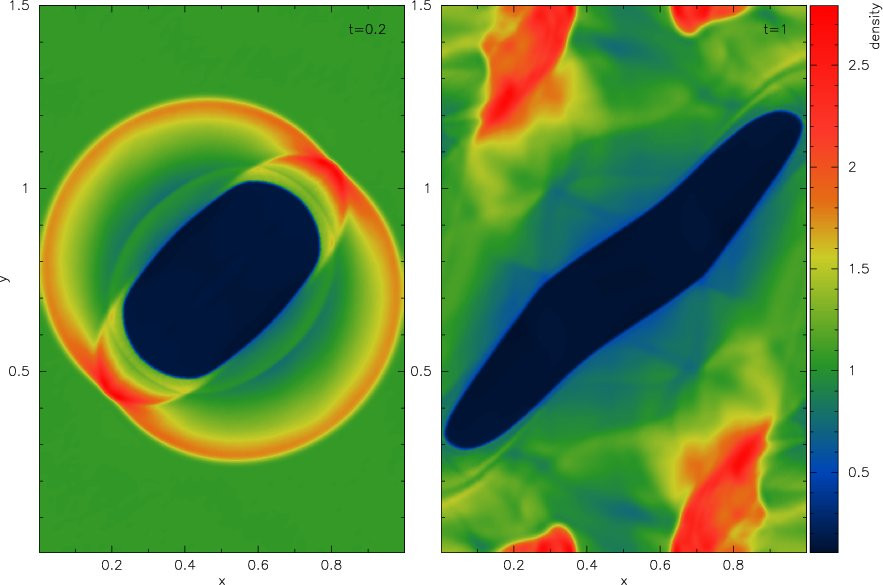
\includegraphics[width=0.8\textwidth]{img/mhd-blast/new/ref.jpg}
	\caption{Reference solution, $\rho$ distribution, $t \approx 0.2$ (left), $t \approx 1.0$ (right), from \cite{blastNew1}}
	\label{figure:blastRef}
	\end{center}
\end{figure}
\vspace{-6mm}
\begin{figure}[H]
	\begin{center}
		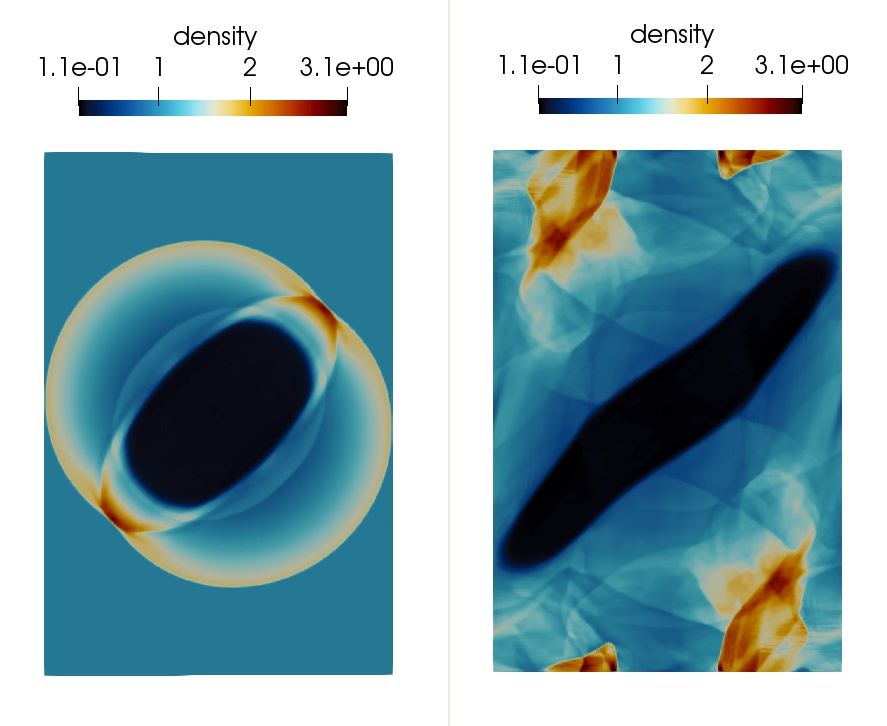
\includegraphics[width=0.8\textwidth]{img/mhd-blast/new/ref-result.jpg}
	\caption{Obtained $\rho$ distribution, $t \approx 0.2$ (left), $t \approx 1.0$ (right)}
	\label{figure:blastFinal}
	\end{center}
\end{figure}
\vspace{-4mm}

\subsubsection{AMR for MHD Blast - extended version}
One can see, that for the finest mesh of $200\times300$ elements, the solution obtained shows very detailed features, and is arguably of even higher quality than the reference one from \cite{blastNew1}. However, the calculation needs
\be
200 \times 300\ = 60000\ \text{elements},
\ee
where each element contains $4$ basis functions for each of $\rho, p, \pi_1, \pi_2, \pi_3$, and $11$ basis functions for $\bfB$, that is $31$ basis functions per element, in total $60000 \times 31 = 1860000$ degrees of freedom (DOFs). This number can be decreased, while keeping the same (or even higher) solution quality, with AMR - as illustrated in \crefrange{figure:amrBlast1}{figure:amrBlast8} below. On each of \crefrange{figure:amrBlast1}{figure:amrBlast8}, the solution is displayed on the left, the adapted mesh in the middle, and the owning processor of a chunk of elements on the right. Note that there were $96$ processors used for the computation.

\begin{figure}[H]
	\begin{center}
		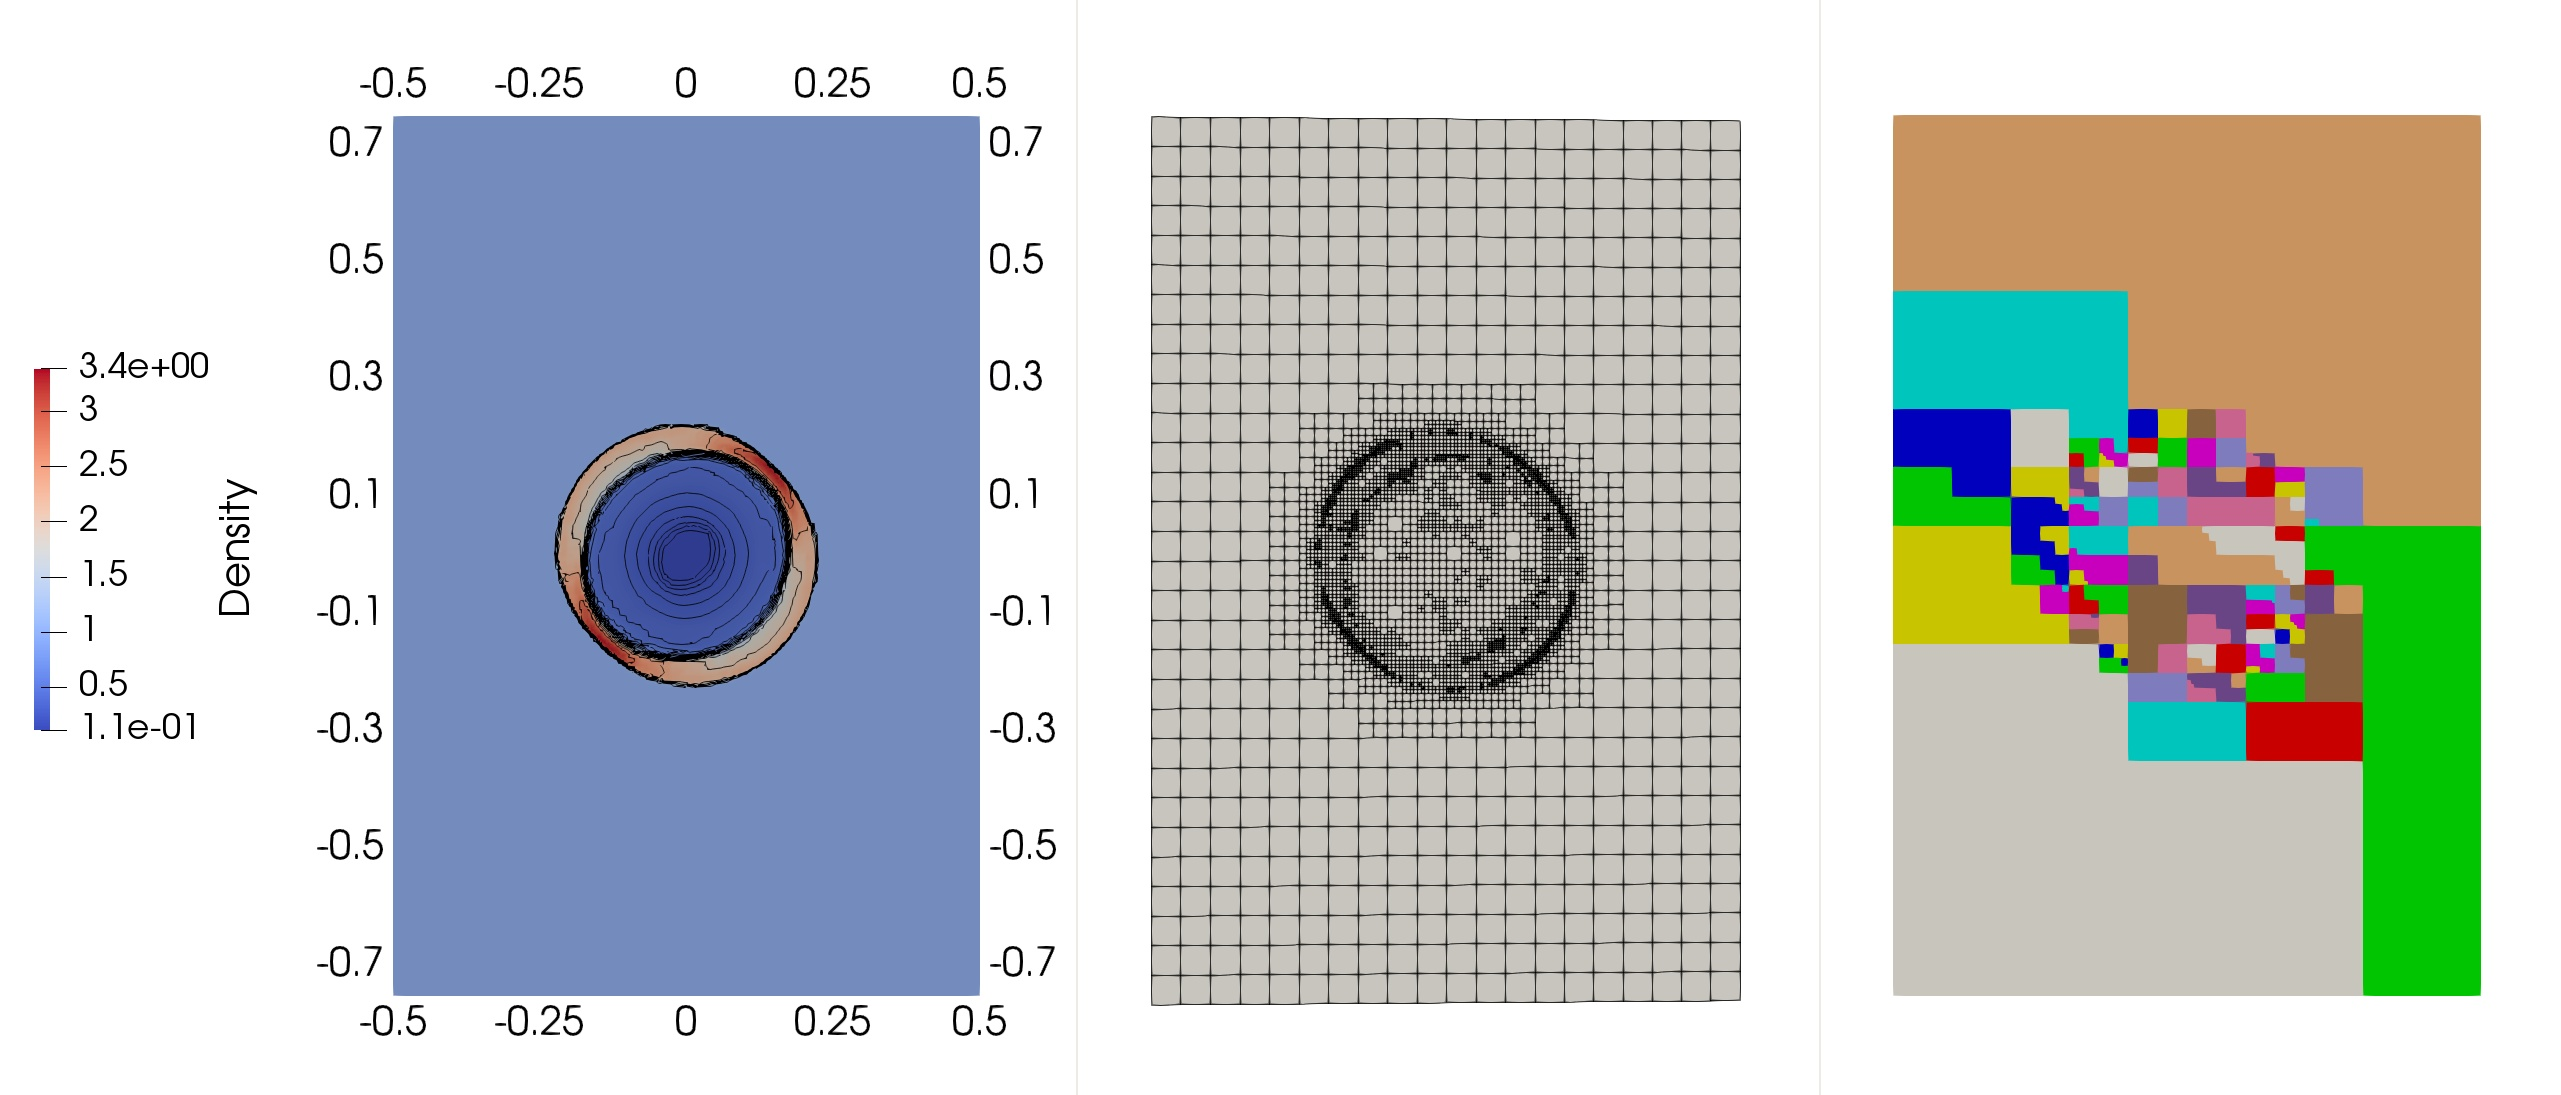
\includegraphics[width=0.8\textwidth]{img/mhd-blast/new/adapt-full0.jpg}
	\caption{Obtained $\rho$ distribution, mesh elements, and their owning processor. Time $t\approx 0.5e-1$.}
	\label{figure:amrBlast1}
	\end{center}
\end{figure}
\vspace{-4mm}

\begin{figure}[H]
	\begin{center}
		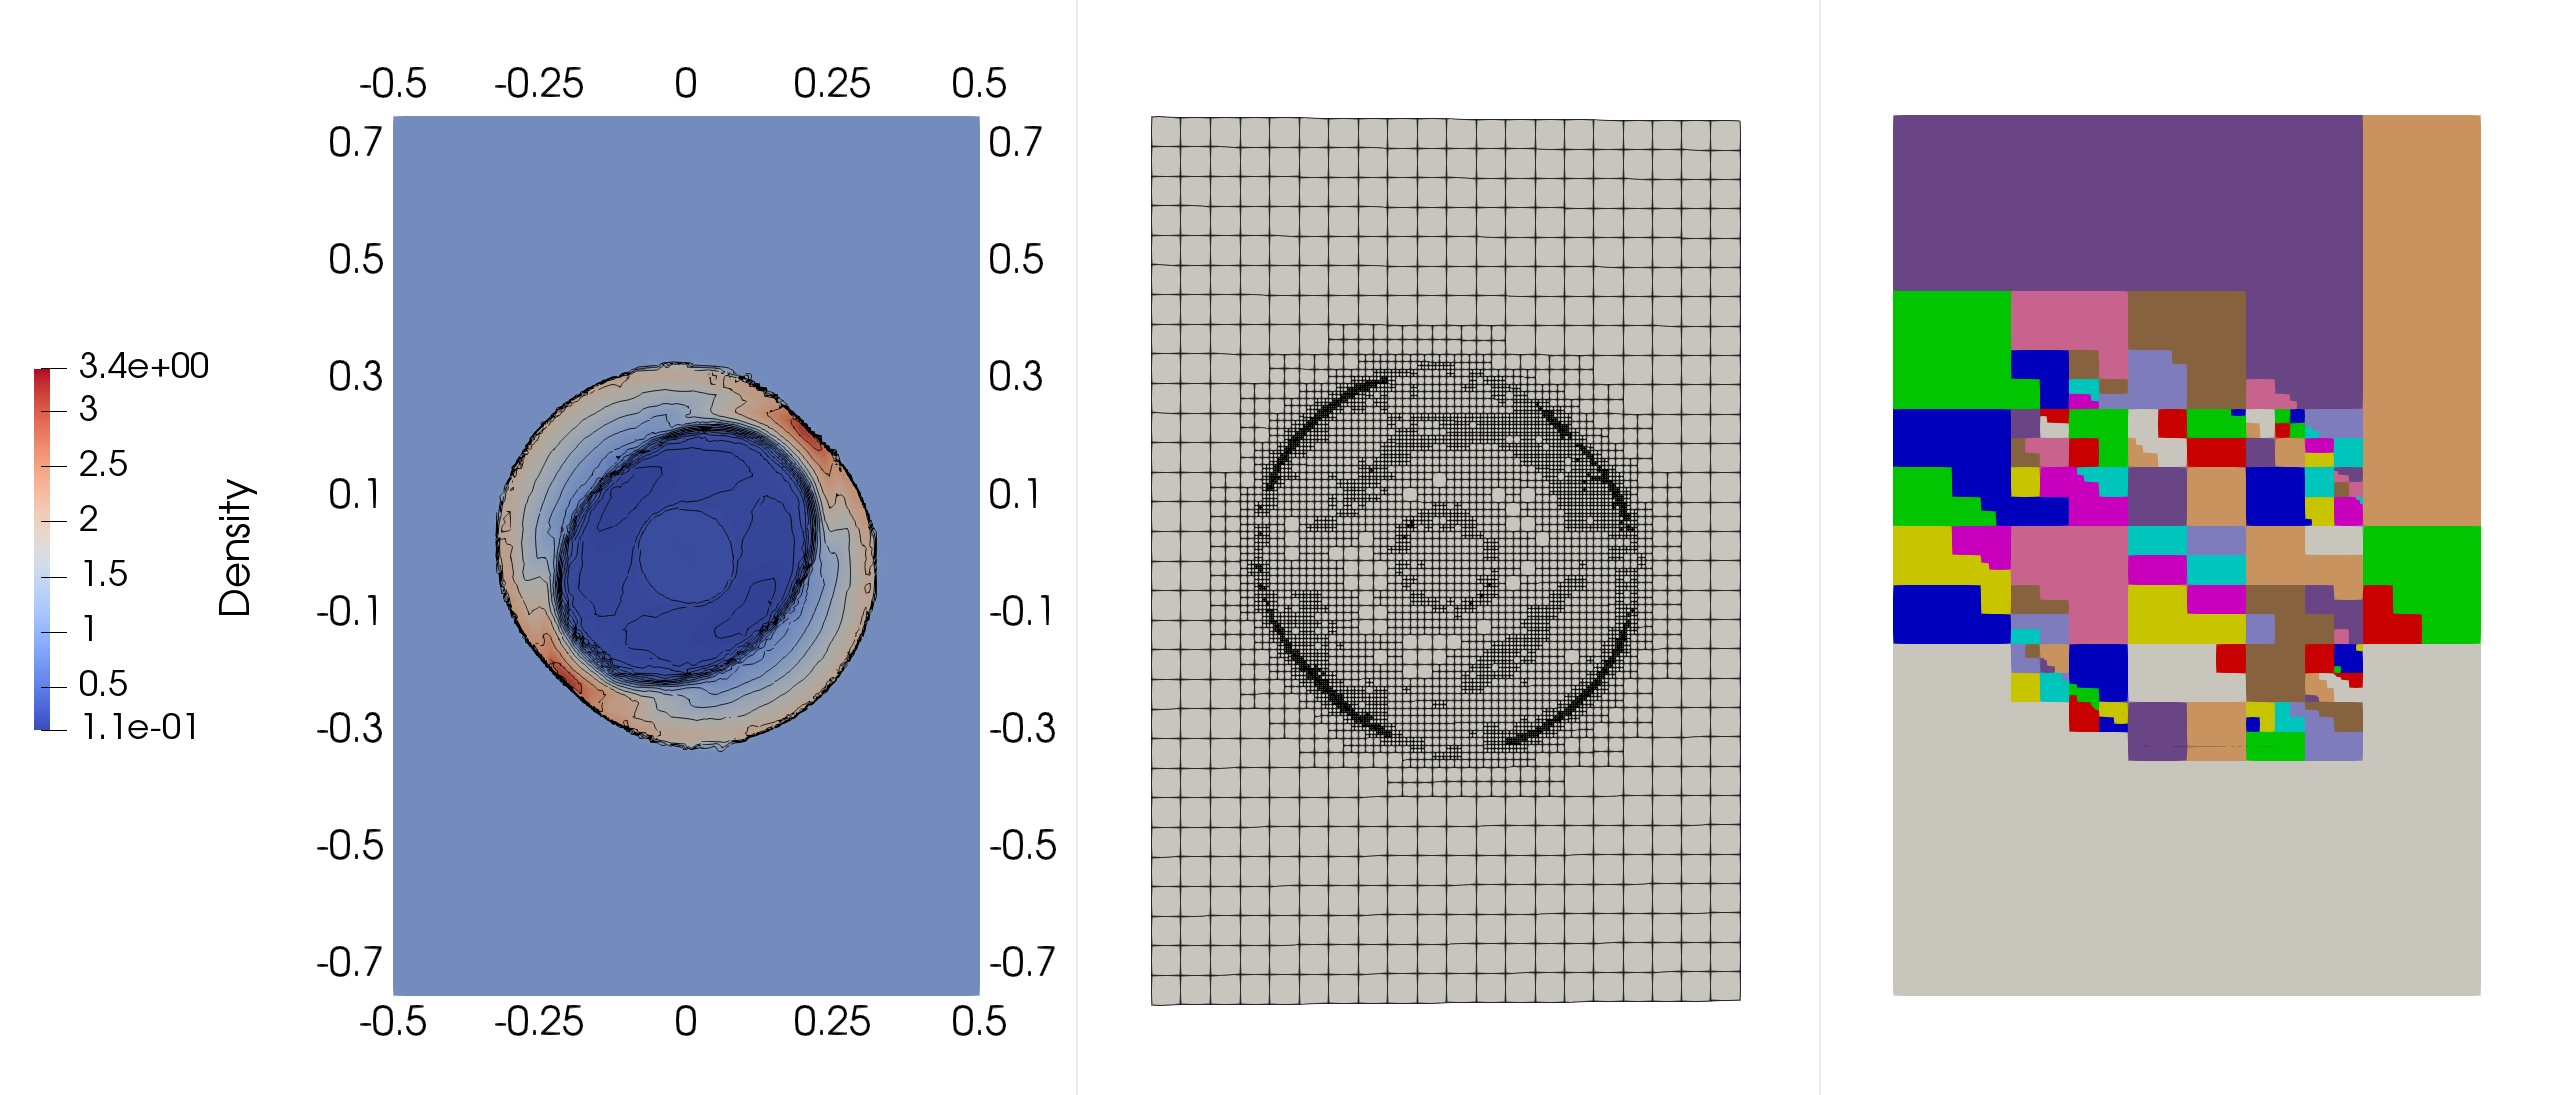
\includegraphics[width=0.8\textwidth]{img/mhd-blast/new/adapt-full1.jpg}
	\caption{Obtained $\rho$ distribution, mesh elements, and their owning processor. Time $t\approx 5e-1$.}
	\label{figure:amrBlast2}
	\end{center}
\end{figure}
\vspace{-4mm}

\begin{figure}[H]
	\begin{center}
		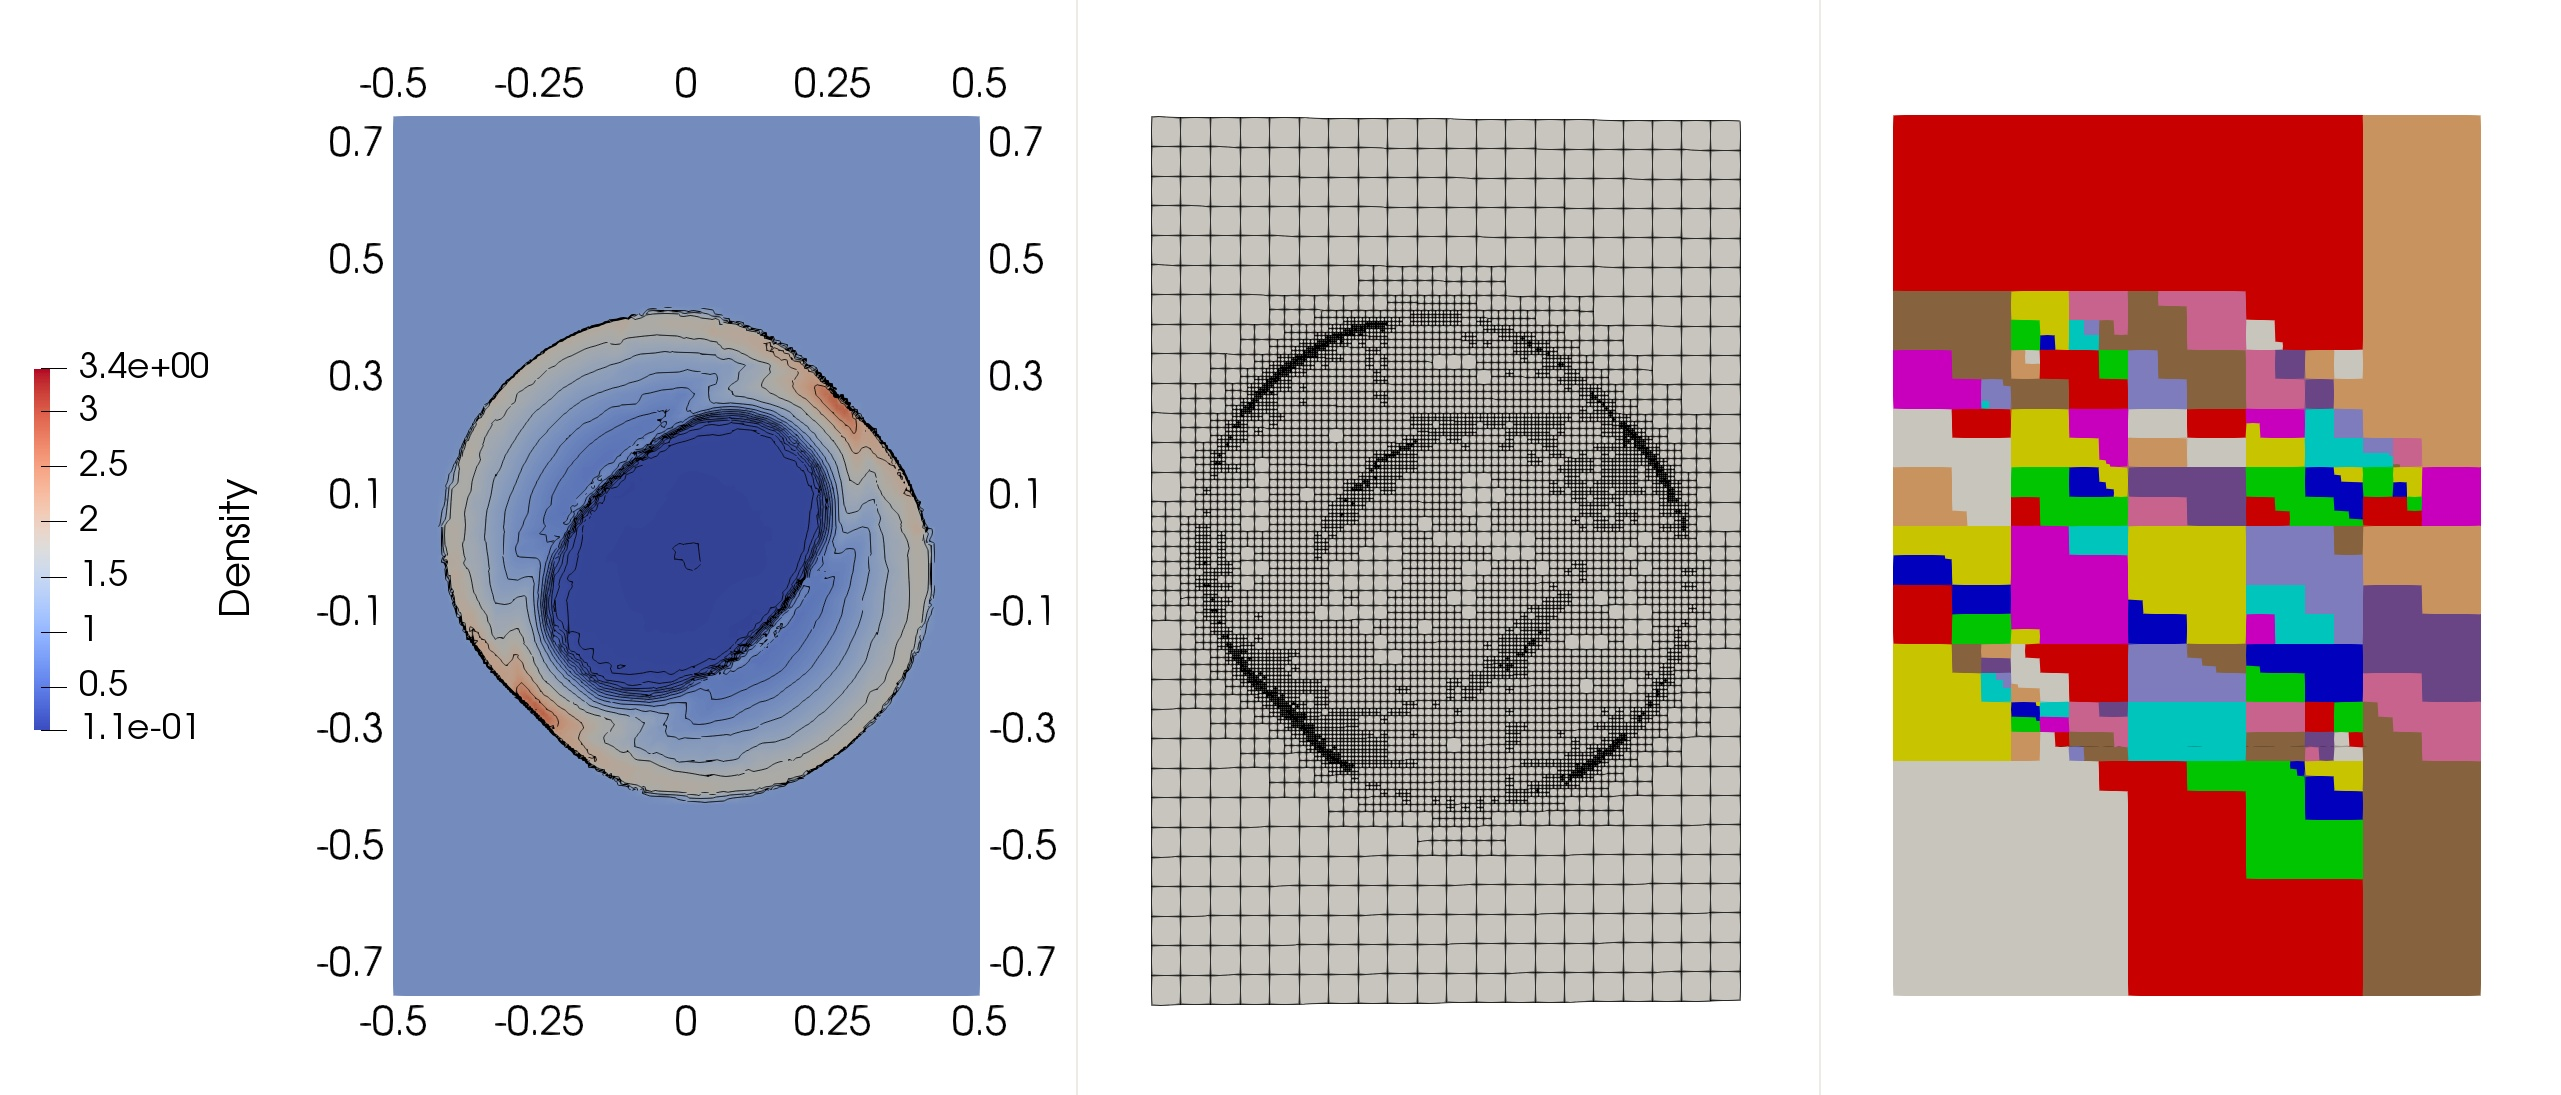
\includegraphics[width=0.8\textwidth]{img/mhd-blast/new/adapt-full2.jpg}
	\caption{Obtained $\rho$ distribution, mesh elements, and their owning processor. Time $t\approx 1.5e-1$.}
	\label{figure:amrBlast3}
	\end{center}
\end{figure}
\vspace{-4mm}

\begin{figure}[H]
	\begin{center}
		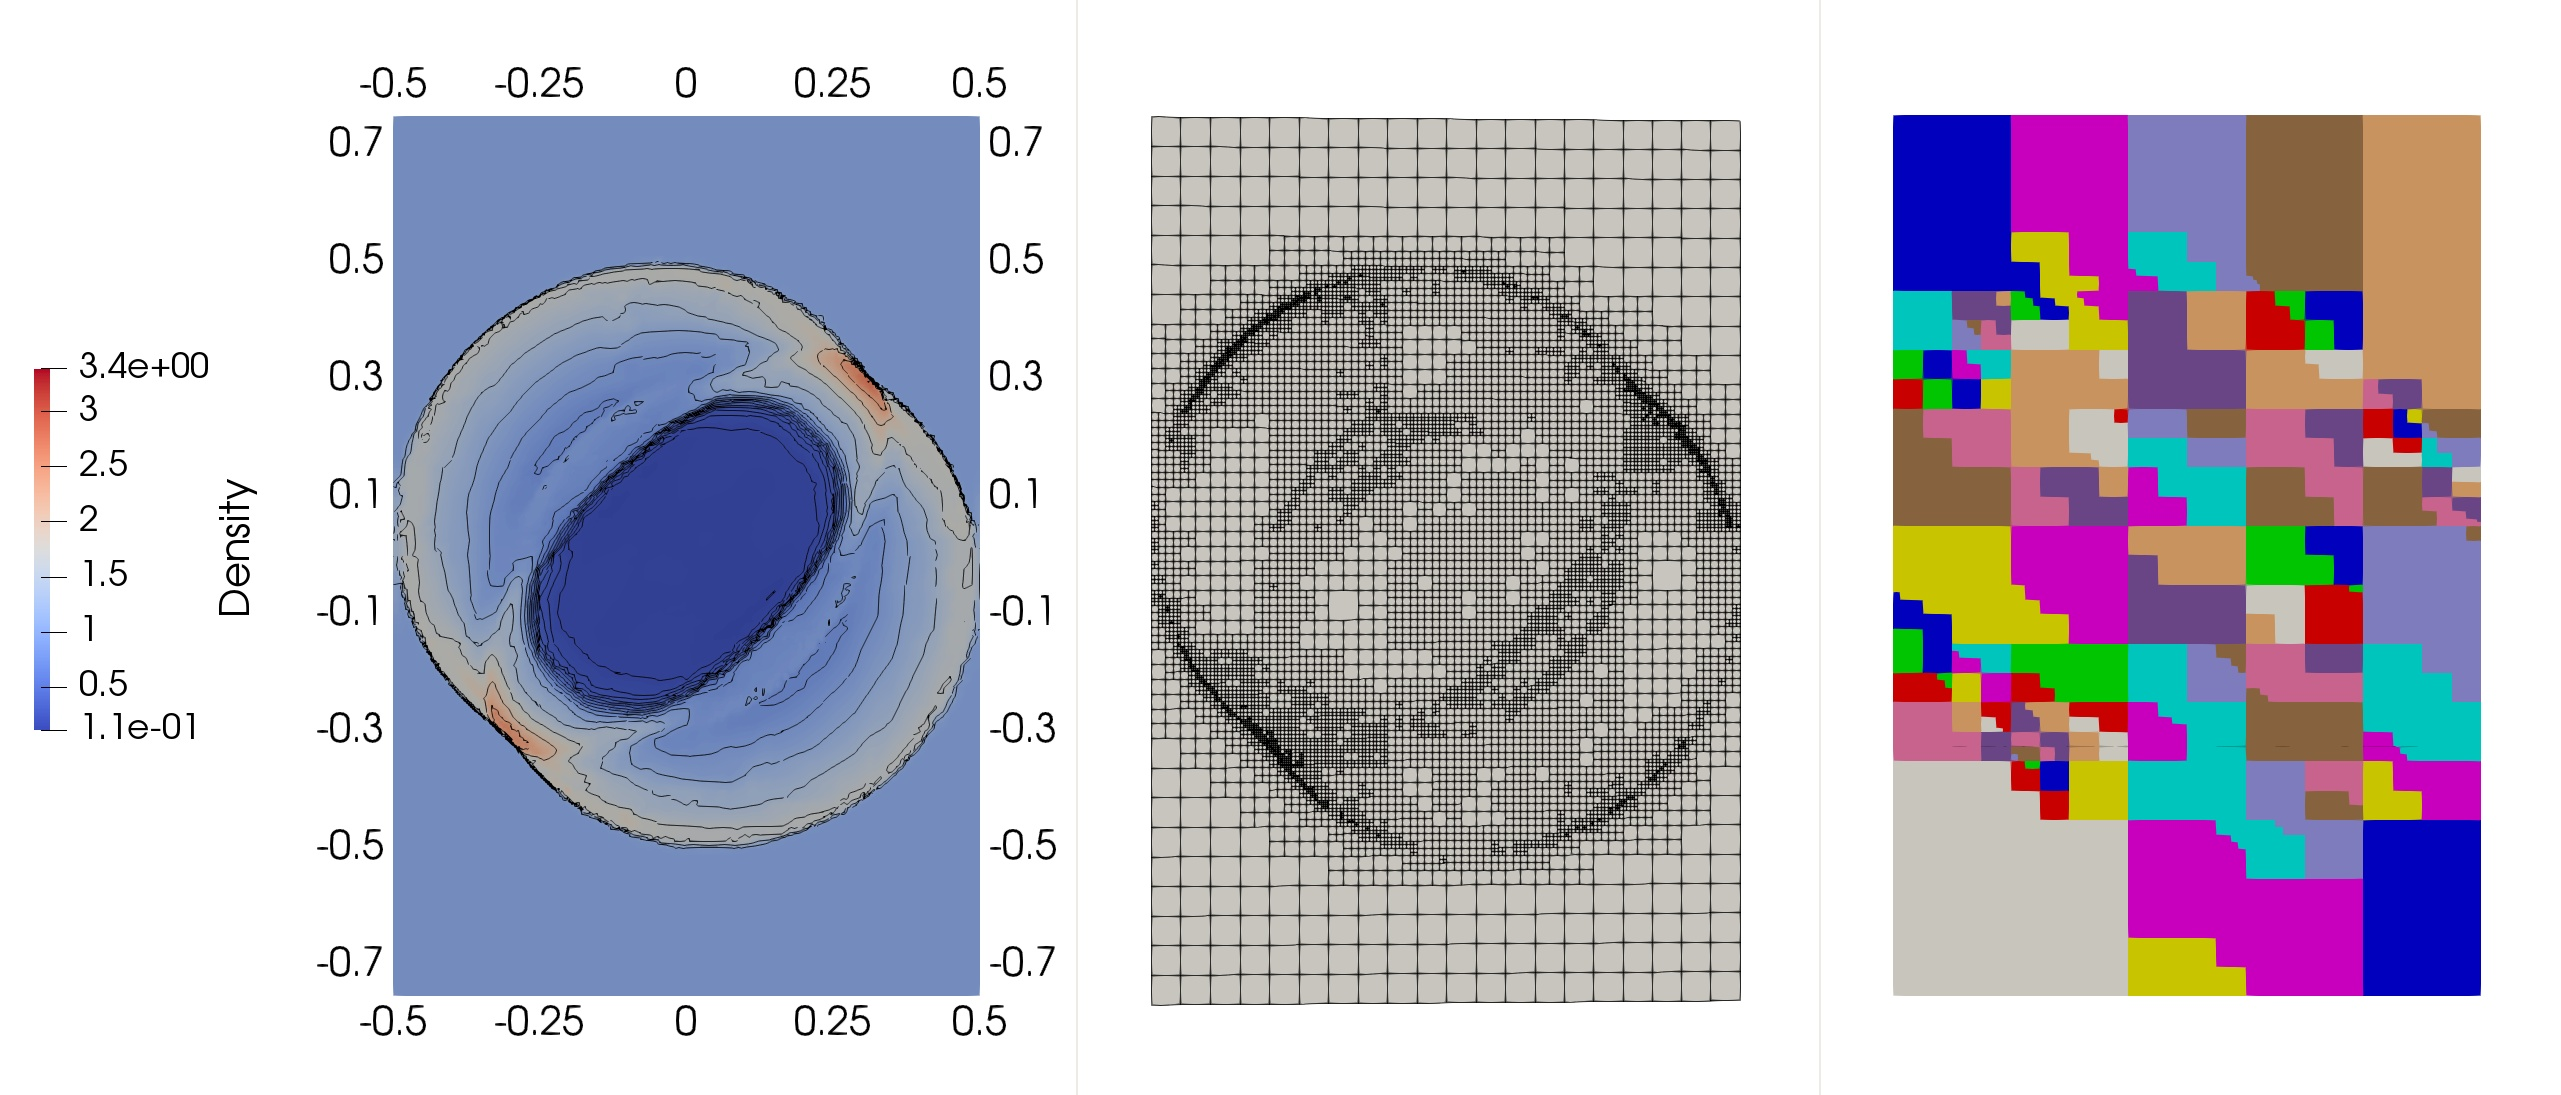
\includegraphics[width=0.8\textwidth]{img/mhd-blast/new/adapt-full3.jpg}
	\caption{Obtained $\rho$ distribution, mesh elements, and their owning processor. Time $t\approx 2e-1$.}
	\label{figure:amrBlast4}
	\end{center}
\end{figure}
\vspace{-4mm}

\begin{figure}[H]
	\begin{center}
		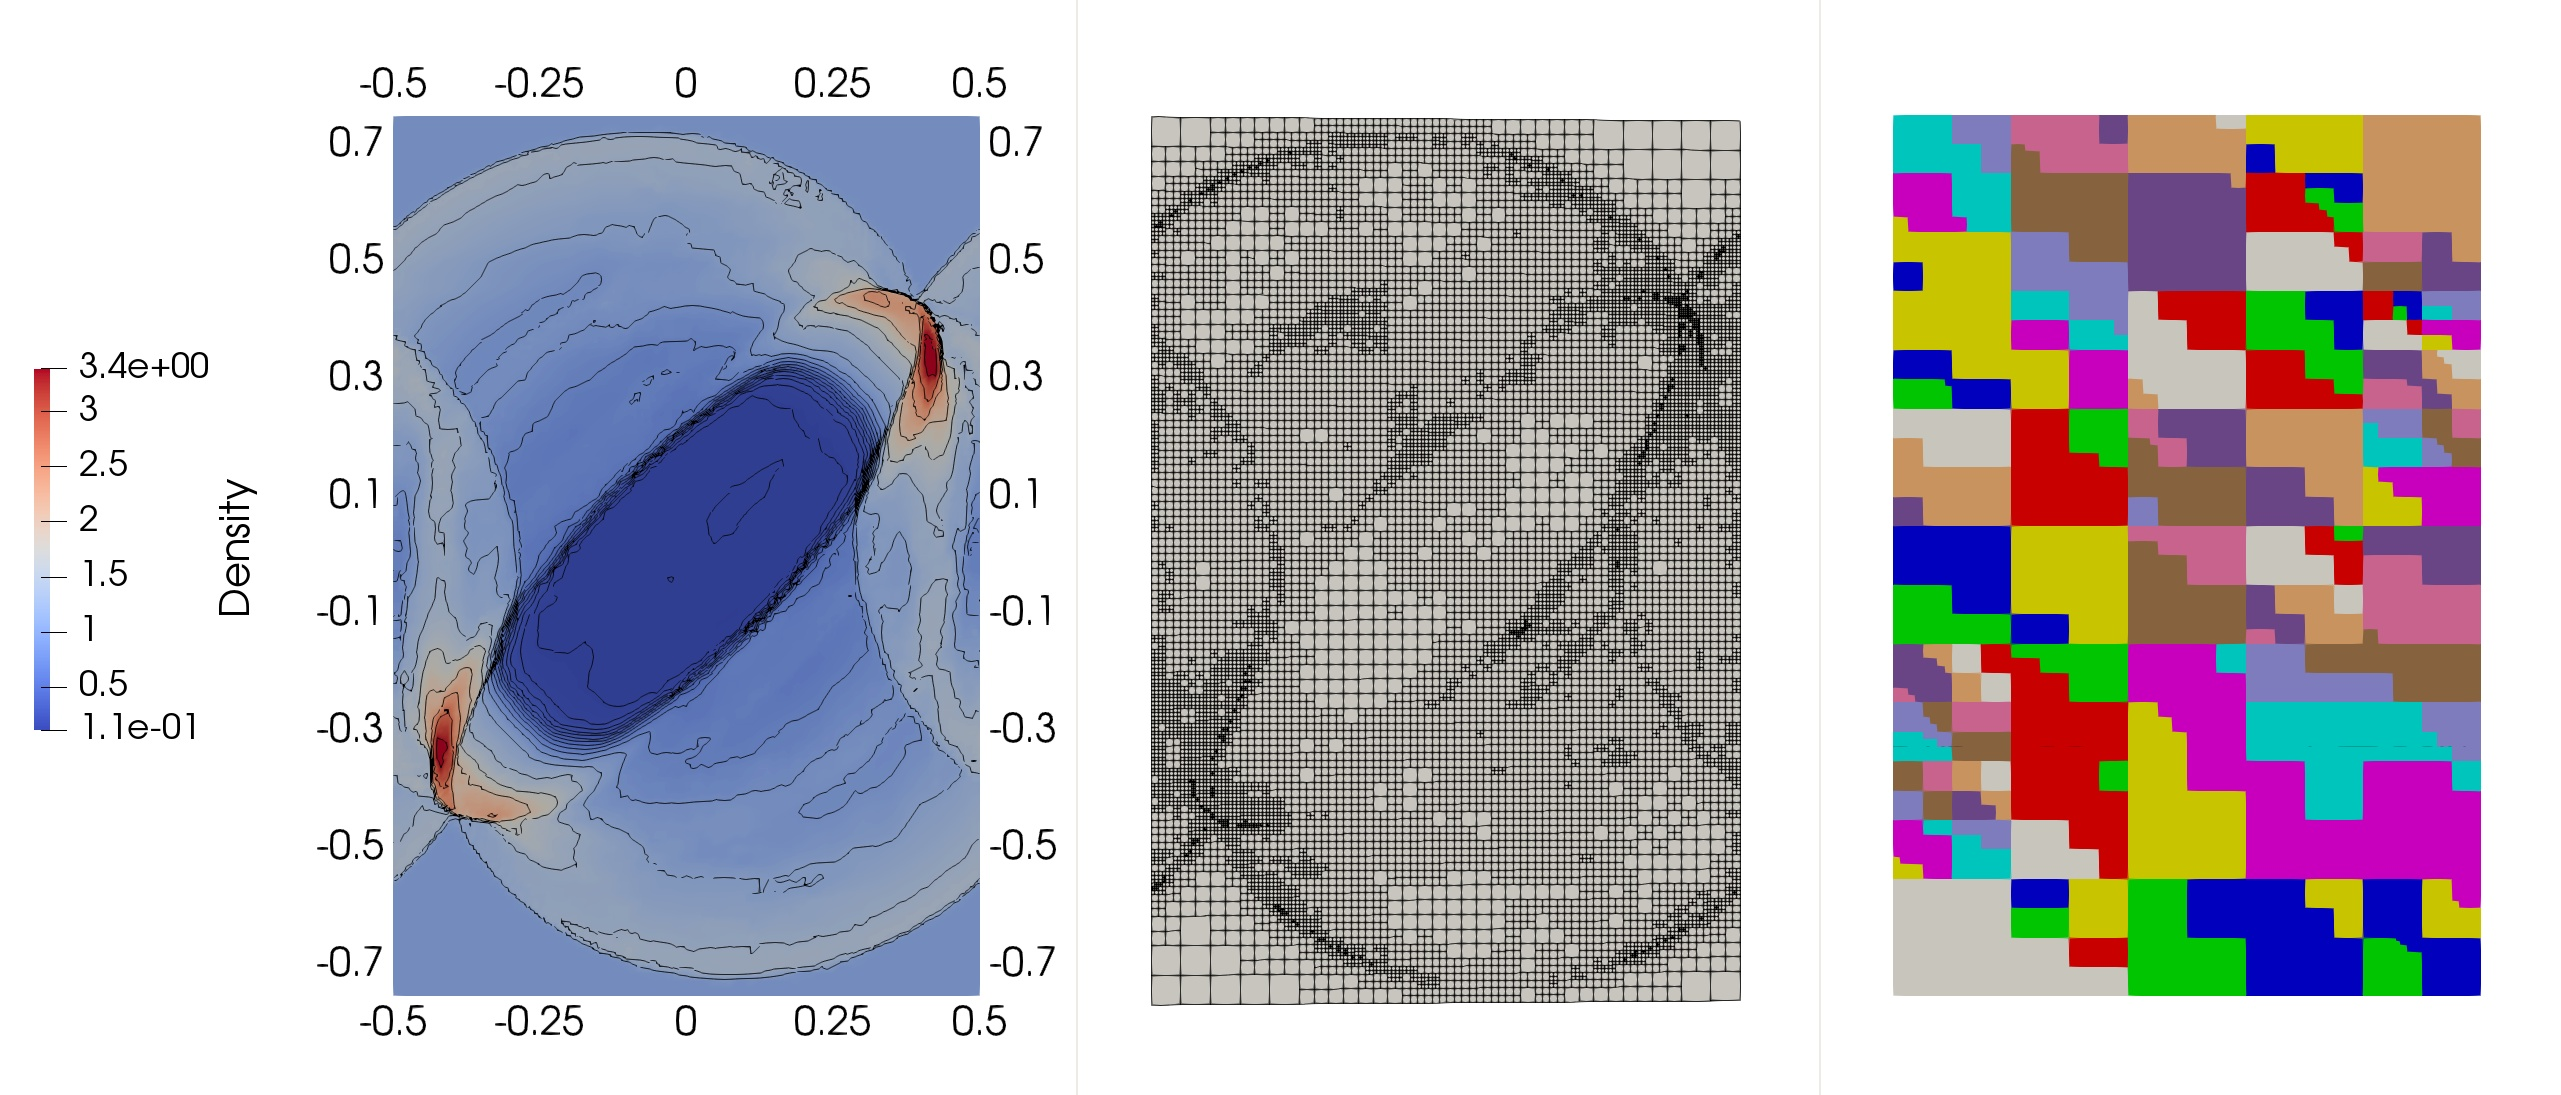
\includegraphics[width=0.8\textwidth]{img/mhd-blast/new/adapt-full6.jpg}
	\caption{Obtained $\rho$ distribution, mesh elements, and their owning processor. Time $t\approx 3.5e-1$.}
	\label{figure:amrBlast5}
	\end{center}
\end{figure}
\vspace{-4mm}

\begin{figure}[H]
	\begin{center}
		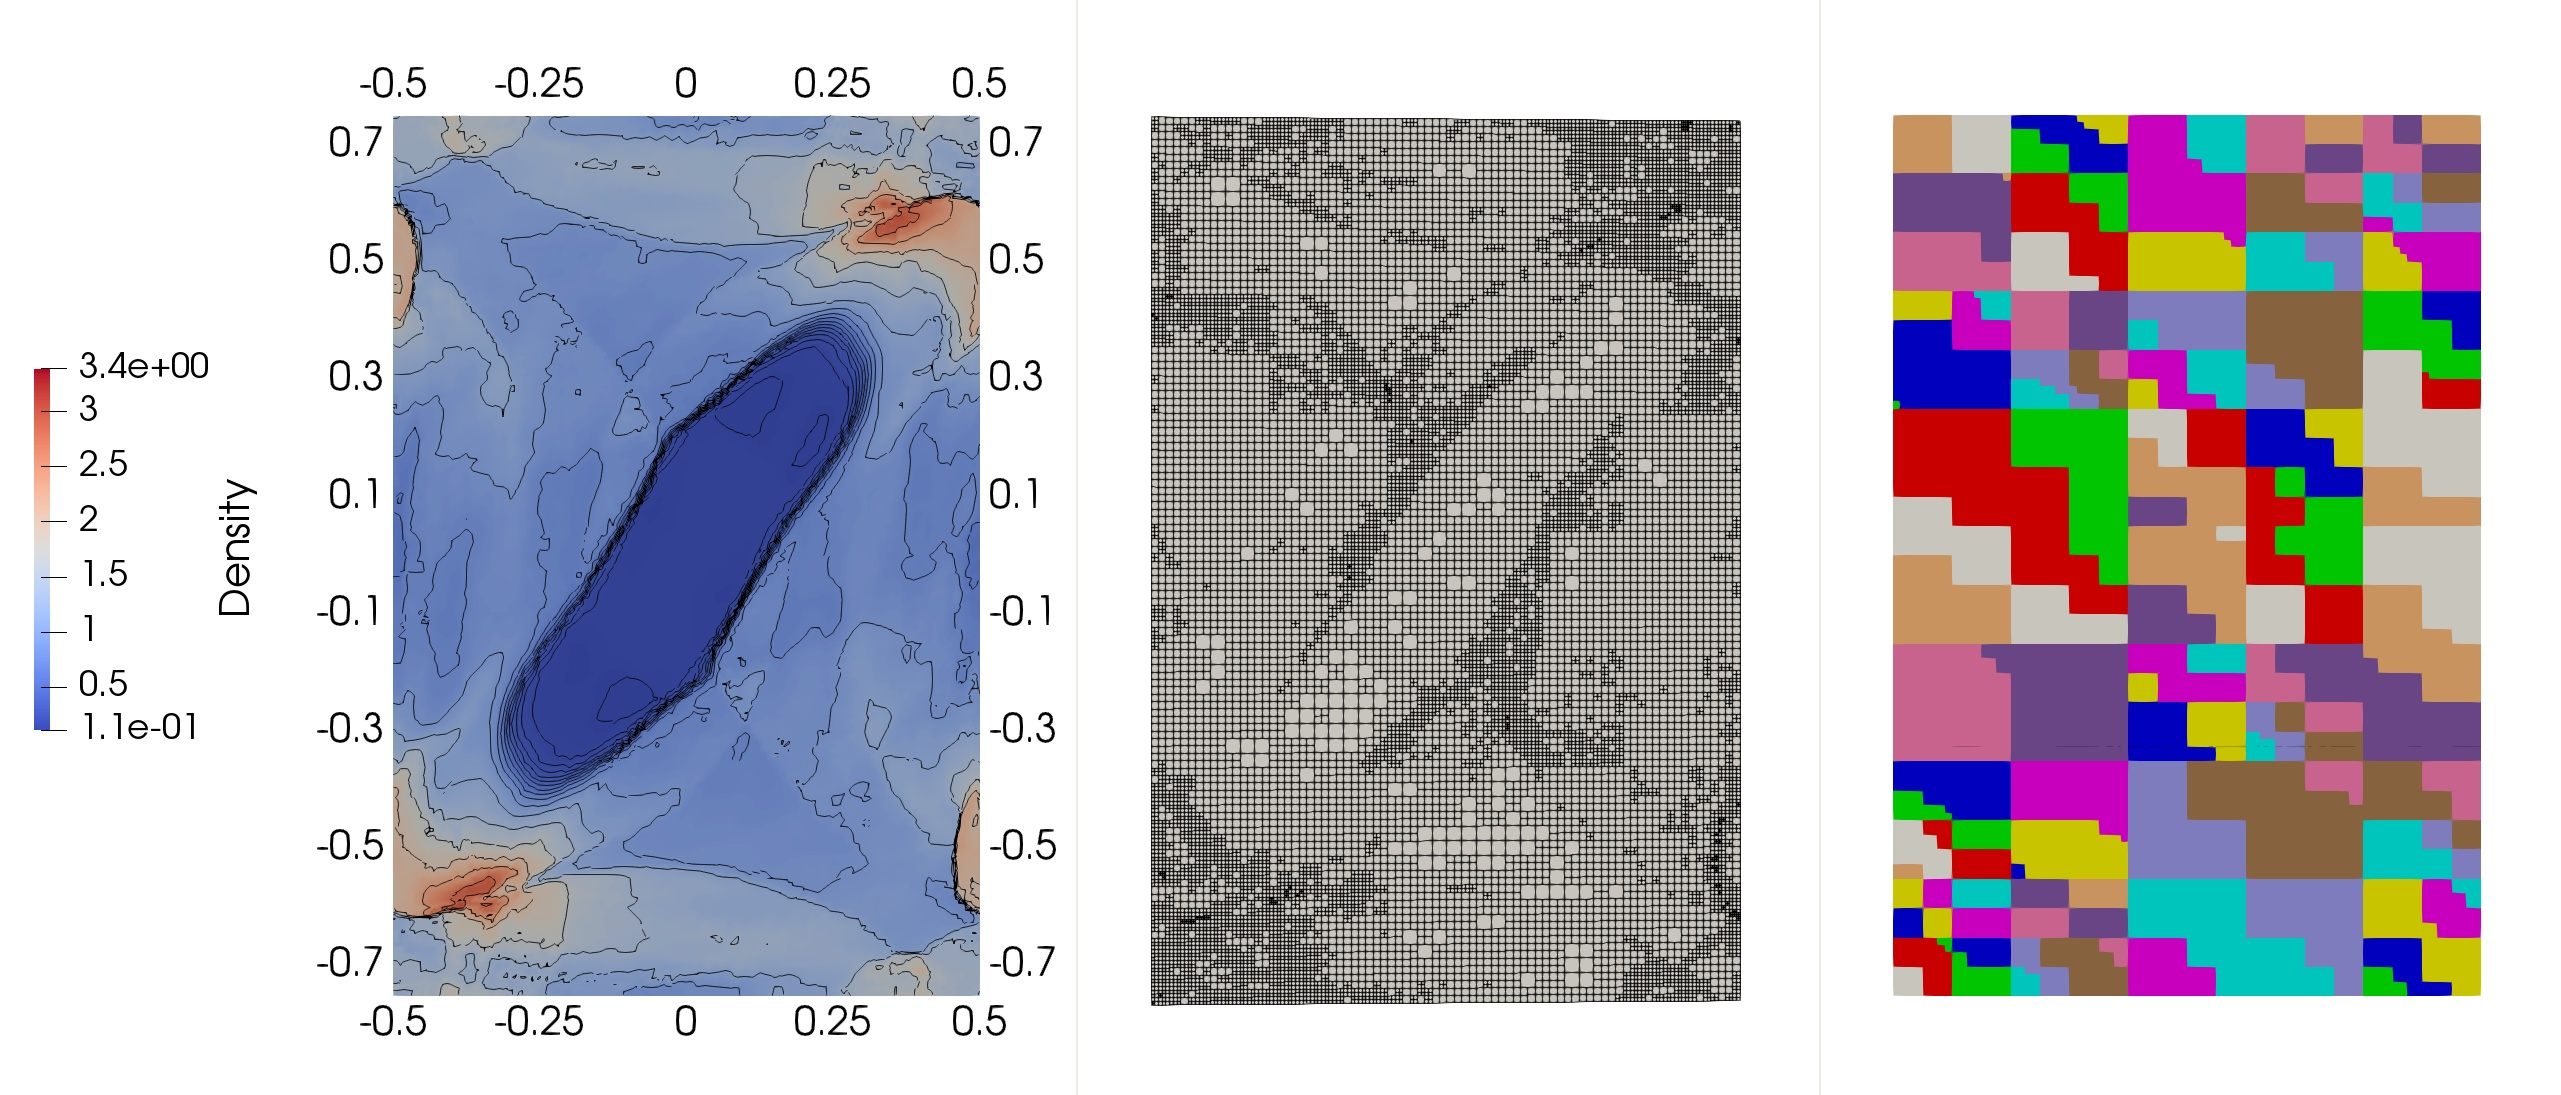
\includegraphics[width=0.8\textwidth]{img/mhd-blast/new/adapt-full10.jpg}
	\caption{Obtained $\rho$ distribution, mesh elements, and their owning processor. Time $t\approx 5.5e-1$.}
	\label{figure:amrBlast6}
	\end{center}
\end{figure}
\vspace{-4mm}


\begin{figure}[H]
	\begin{center}
		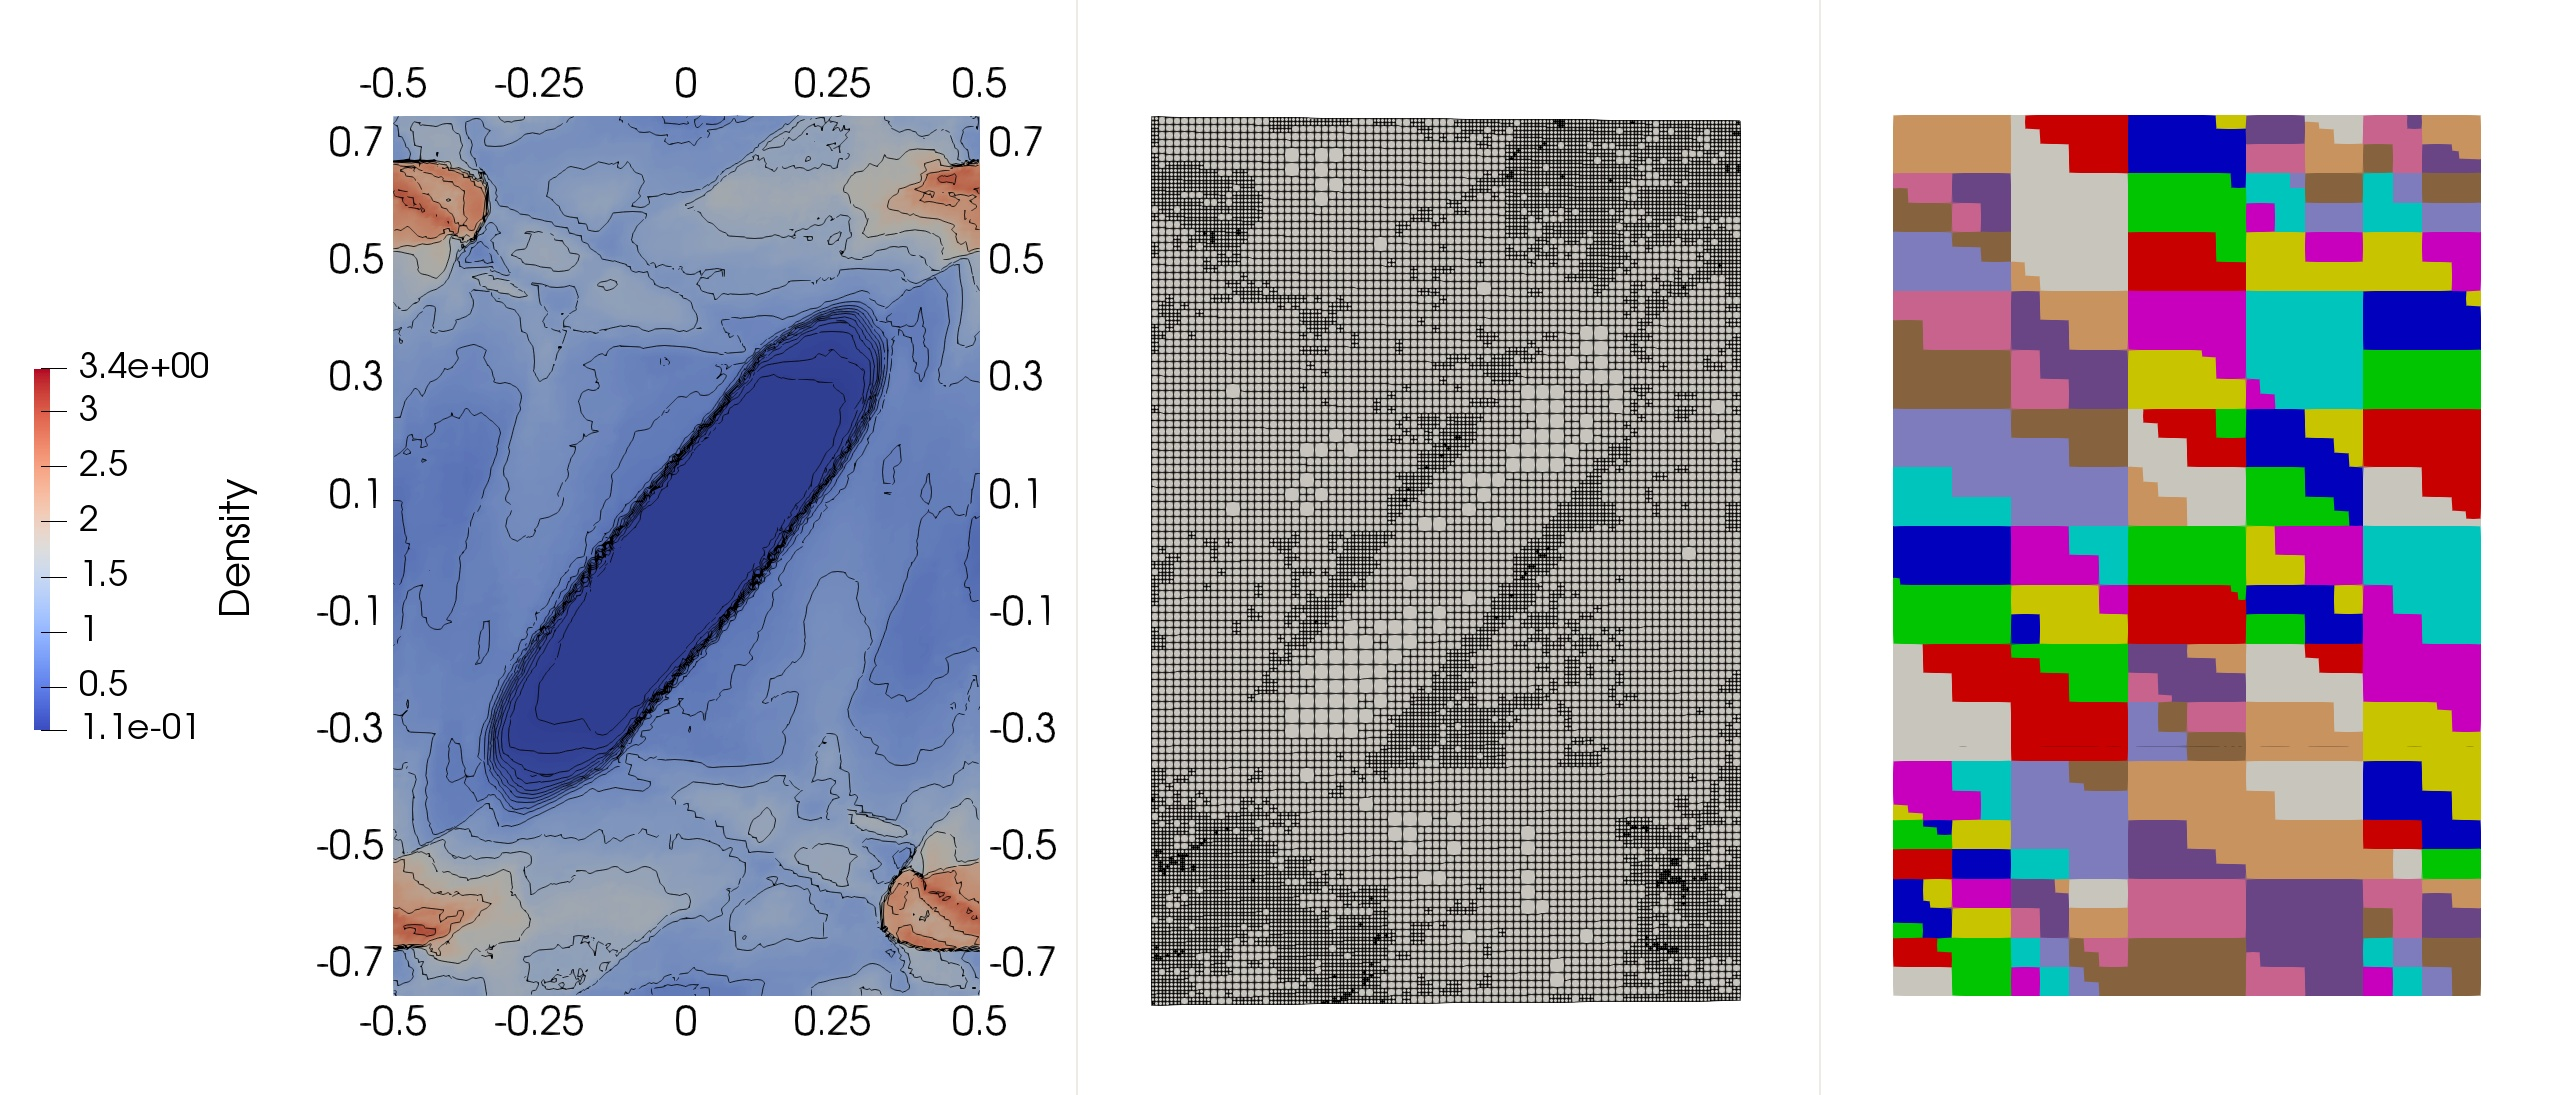
\includegraphics[width=0.8\textwidth]{img/mhd-blast/new/adapt-full13.jpg}
	\caption{Obtained $\rho$ distribution, mesh elements, and their owning processor. Time $t\approx 7e-1$.}
	\label{figure:amrBlast7}
	\end{center}
\end{figure}
\vspace{-4mm}


\begin{figure}[H]
	\begin{center}
		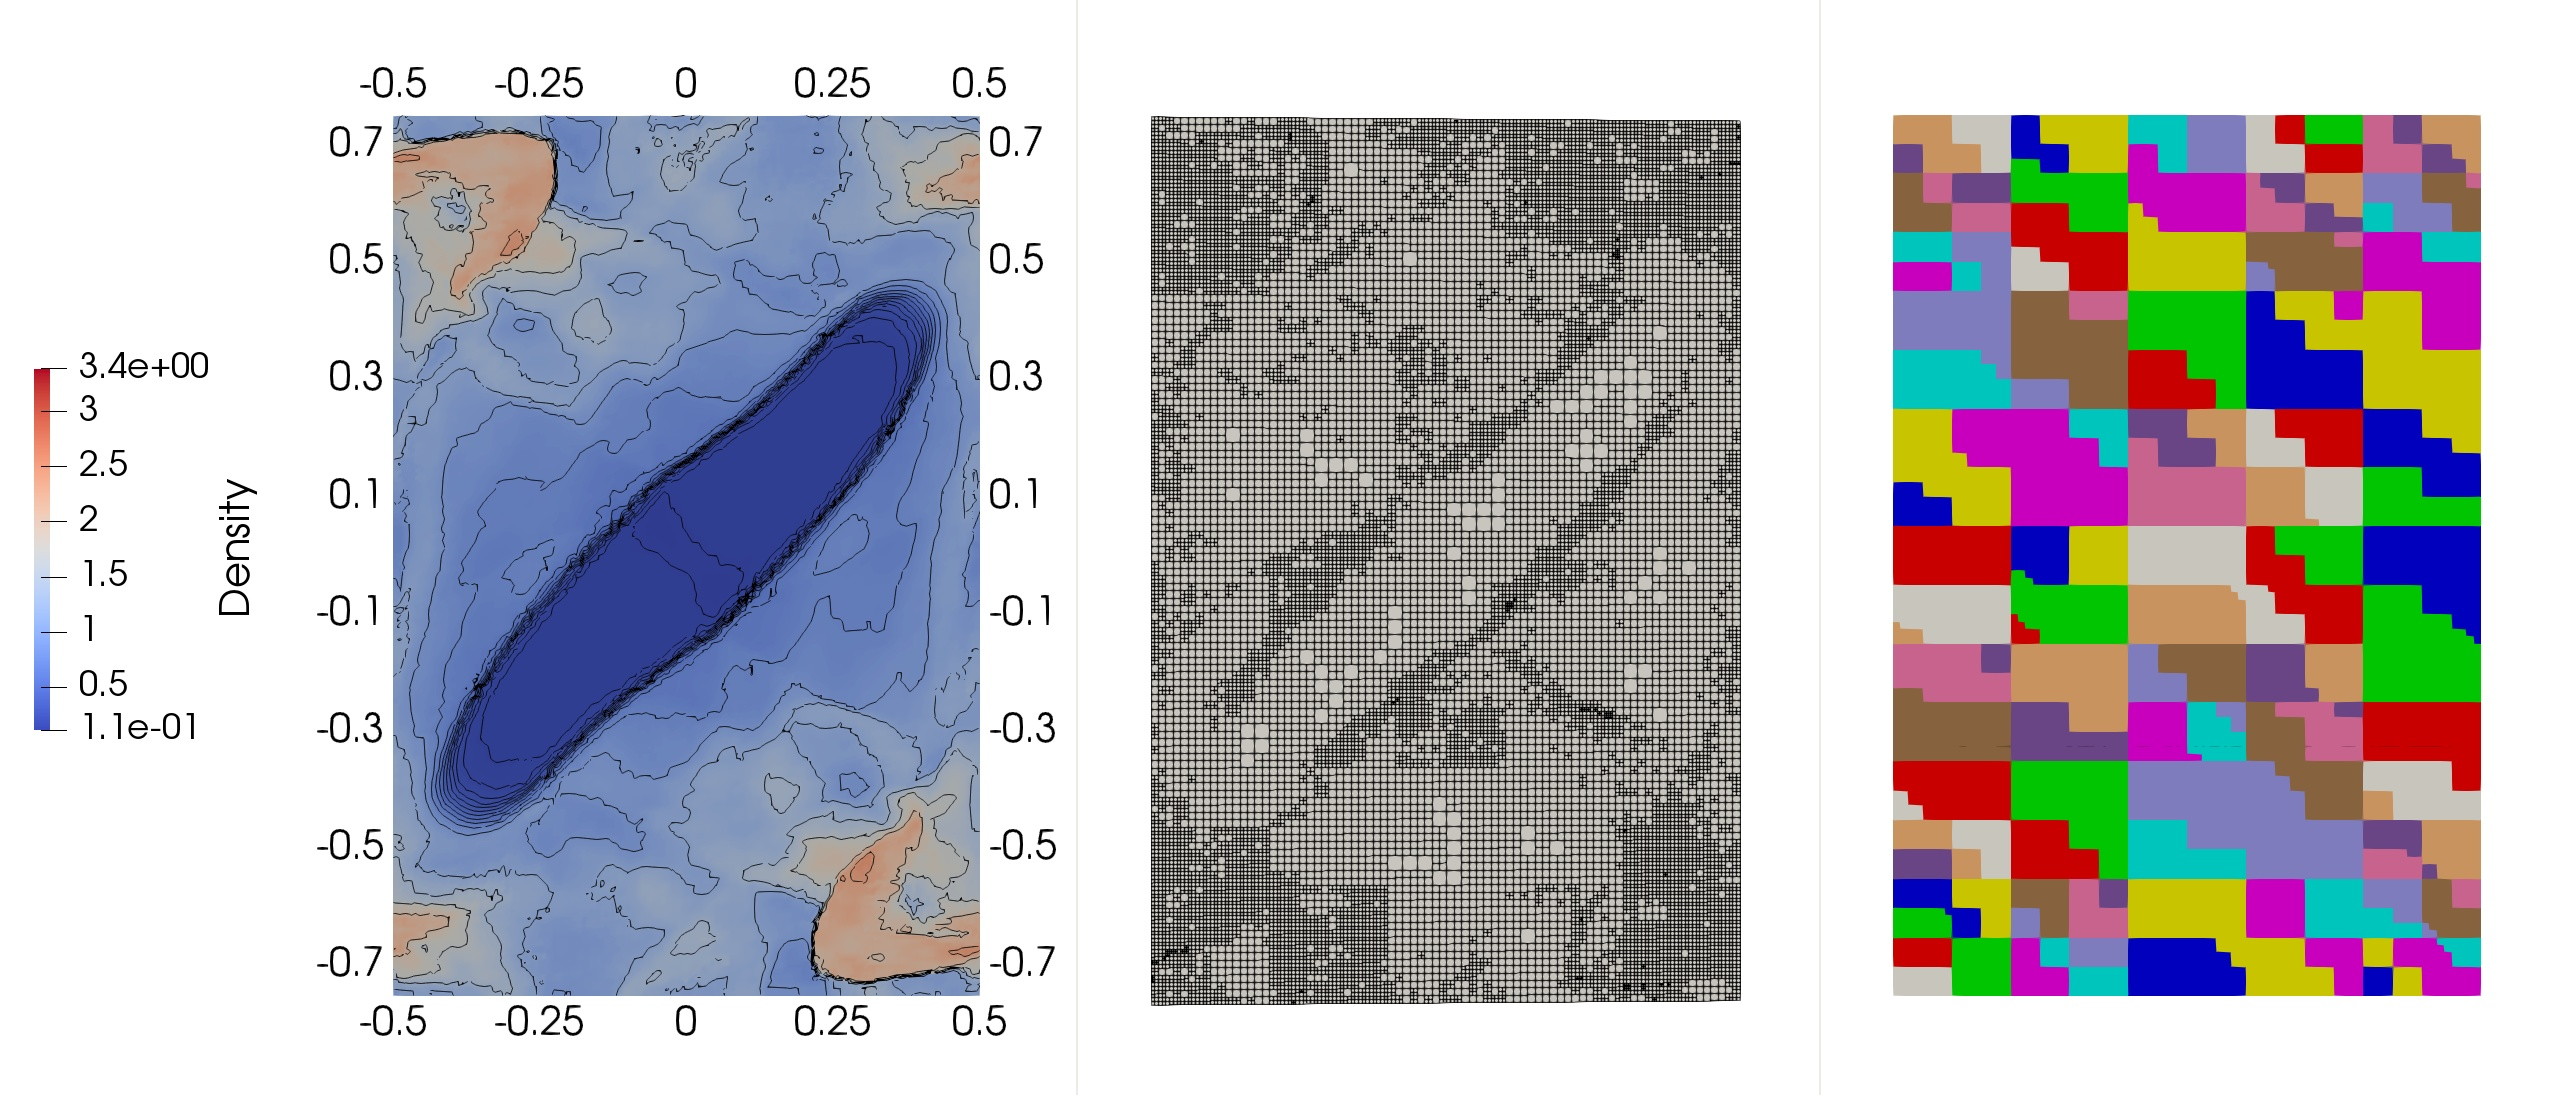
\includegraphics[width=0.8\textwidth]{img/mhd-blast/new/adapt-full16.jpg}
	\caption{Obtained $\rho$ distribution, mesh elements, and their owning processor. Time $t\approx 8.5e-1$.}
	\label{figure:amrBlast8}
	\end{center}
\end{figure}
\vspace{-4mm}
In the \cref{table:meshElems}, mesh elements counts for all the displayed snapshots are given. Note that, as described in \cref{algorithm:AMRFull}, the number of elements constantly evolves.

\begin{table}
    \begin{tabular}
		{ | l | l | p{5cm} |}
		\hline
    \textbf{Time step} & \textbf{Number of mesh elements} & \textbf{Number of DOFs} \\
		\hline
    $t\approx 0.5e-1$ & 5880 & 182280  \\ \hline
    $t\approx 1e-1$ & 7332 & 227292  \\ \hline
    $t\approx 1.5e-1$ & 8649 & 268119  \\ \hline
    $t\approx 2e-1$ & 10044 & 311364  \\ \hline
    $t\approx 3.5e-1$ & 14013 & 434403  \\ \hline
    $t\approx 5.5e-1$ & 16578  & 513918 \\ \hline
    $t\approx 7e-1$ & 17192 & 532952  \\ \hline
    $t\approx 8.5e-1$ & 18708 & 579948  \\ \hline
    \end{tabular}
	\caption{Mesh elements and DOFs counts for snapshots displayed in \crefrange{figure:amrBlast1}{figure:amrBlast8}}
\label{table:meshElems}
\end{table}

From \cref{table:meshElems}, it is cleary visible, that even for such a complex, and seemingly chaotic example, the AMR approach can cut down the number of mesh elements / DOFs radically, by 70-90 \%, while achieving comparable results. 

\subsection{Orszag-Tang vortex}
This problem was first described in \cite{vortex} and has been extensively used as a benchmark for 2- and 3- dimensional MHD code (\cite{blast0}, \cite{blast1}, \cite{honzaFem}, \cite{otnew}, and many others). It is a simple model of the evolution of MHD turbulence including interactions between the several shock waves that appear. The Orszag-Tang system is defined by the initial conditions:
\begin{align}
\rho_0 & =  \frac{25}{36 \pi}\\ \nonumber
p_0 & =  \frac{5}{12 \pi}\\  \nonumber
B_0 & =  \sqrt{\frac{1}{4 \pi}}\\ \nonumber
\gamma & =  5 / 3\\ \nonumber
\rho\lo\bfx, t = 0\ro & =  \rho_0,\\ \nonumber
p\lo\bfx, t = 0\ro & =  p_0,\\ \nonumber
\bfu_1\lo\bfx, t = 0\ro & =  -\sin(2 \pi y),\\ \nonumber
\bfu_2\lo\bfx, t = 0\ro & =  \sin(2 \pi x),\\ \nonumber
\bfu_3\lo\bfx, t = 0\ro & =  0,\\ \nonumber
\bfB_1\lo\bfx, t = 0\ro & =  -B_0 \sin(2 \pi y),\\ \nonumber
\bfB_2\lo\bfx, t = 0\ro & =  B_0 \sin(4 \pi x),\\ \nonumber
\bfB_3\lo\bfx, t = 0\ro & =  0,\\ \nonumber
U\lo\bfx, t = 0\ro & =  \frac{p_0}{\gamma - 1} + U_m\lo\bfx, t\ro + U_k\lo\bfx, t\ro,
\end{align}
where the last term is an application of \cref{magU,kinU,presU}. The domain $\Omega$ is set as $\Omega = [0, 1] \times [0, 1]$ and the problem is equipped with periodic boundary conditions on the top-bottom, and left-right parts of the boundary, similarly as in \cref{sec:blastNew}. This configuration is strongly unstable, leading to a wide spectrum of propagating MHD modes and shock waves.
\paragraph{}
As before, in order to compare with reference papers, figures are presented from these papers - see \cref{figure:otRef}. The images are taken from pages 30 (\cite{blast1}), and 20/282 (\cite{blast0}) respectively. All are taken at $t = 0.5$.

\begin{figure}[H]
\centering
\begin{subfigure}[b]{0.4\textwidth}\vspace{12mm}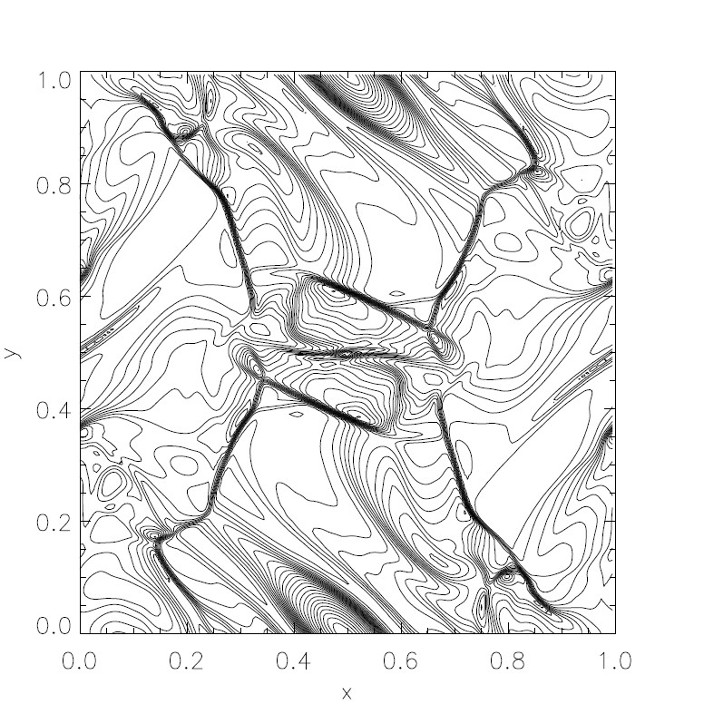
\includegraphics[width=\textwidth]{img/ot/ref-londrillo-pressure.jpg}\end{subfigure}
\begin{subfigure}[b]{0.4\textwidth}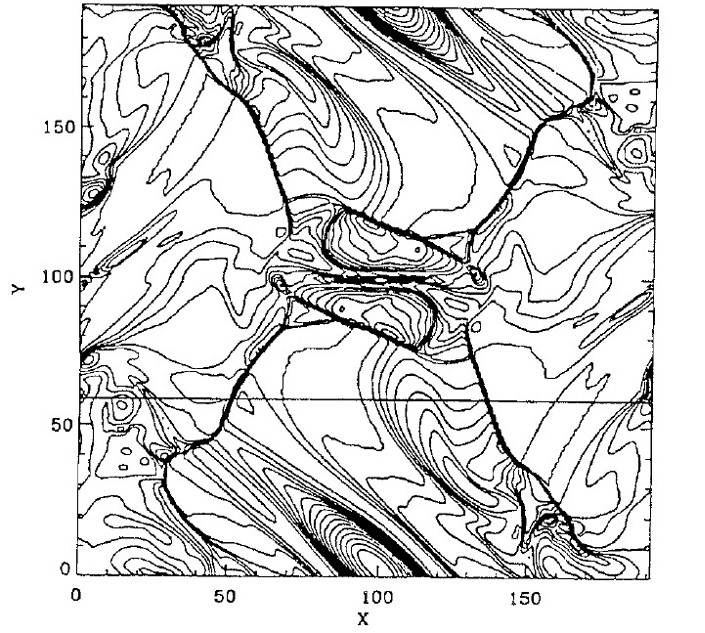
\includegraphics[width=\textwidth]{img/ot/ref-zachary-pressure-contour.jpg}\end{subfigure}
\\
\begin{subfigure}[b]{0.75\textwidth}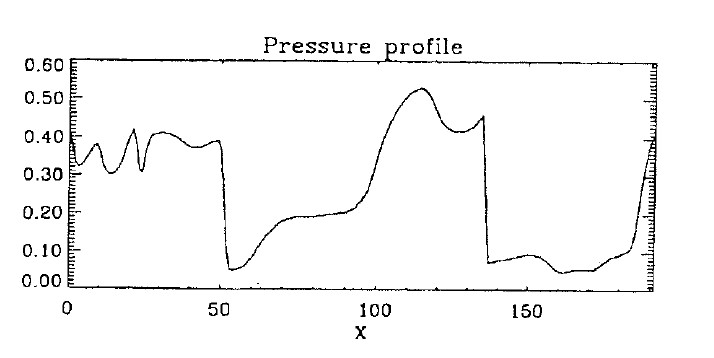
\includegraphics[width=\textwidth]{img/ot/ref-zachary-pressure-profile.jpg}\end{subfigure}
\caption{$p$ isolines from \cite{blast1} (top left), $p$ isolines from \cite{blast0} (top right), $p$ along $y = 0.3125$ from \cite{blast0} (bottom).}
\label{figure:otRef}
\end{figure}

Results obtained in the implemented software are presented in \crefrange{figure:myOt1}{figure:myOt7}. The result on \cref{figure:myOt7} is obviously in almost exact accordance with \cref{figure:otRef}.

\begin{figure}[H]
	\centering
	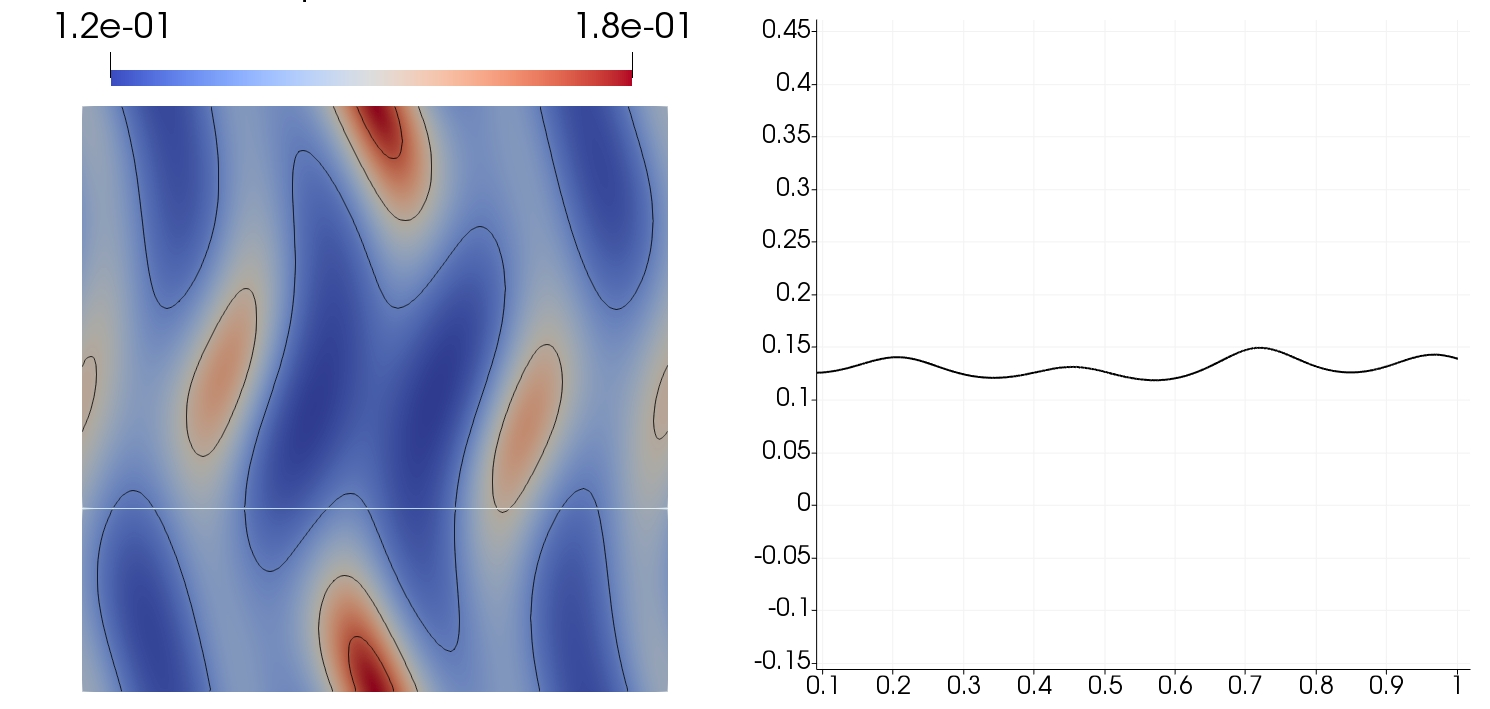
\includegraphics[width=0.92\textwidth]{img/ot/my1new.jpg}
\vspace{-2mm}
\caption{$p$ distribution in $\Omega$ and $p$ along $y = 0.3125$, $t = 0.03$}
\label{figure:myOt1}
\end{figure}
\vspace{-4mm}

\begin{figure}[H]
	\centering
	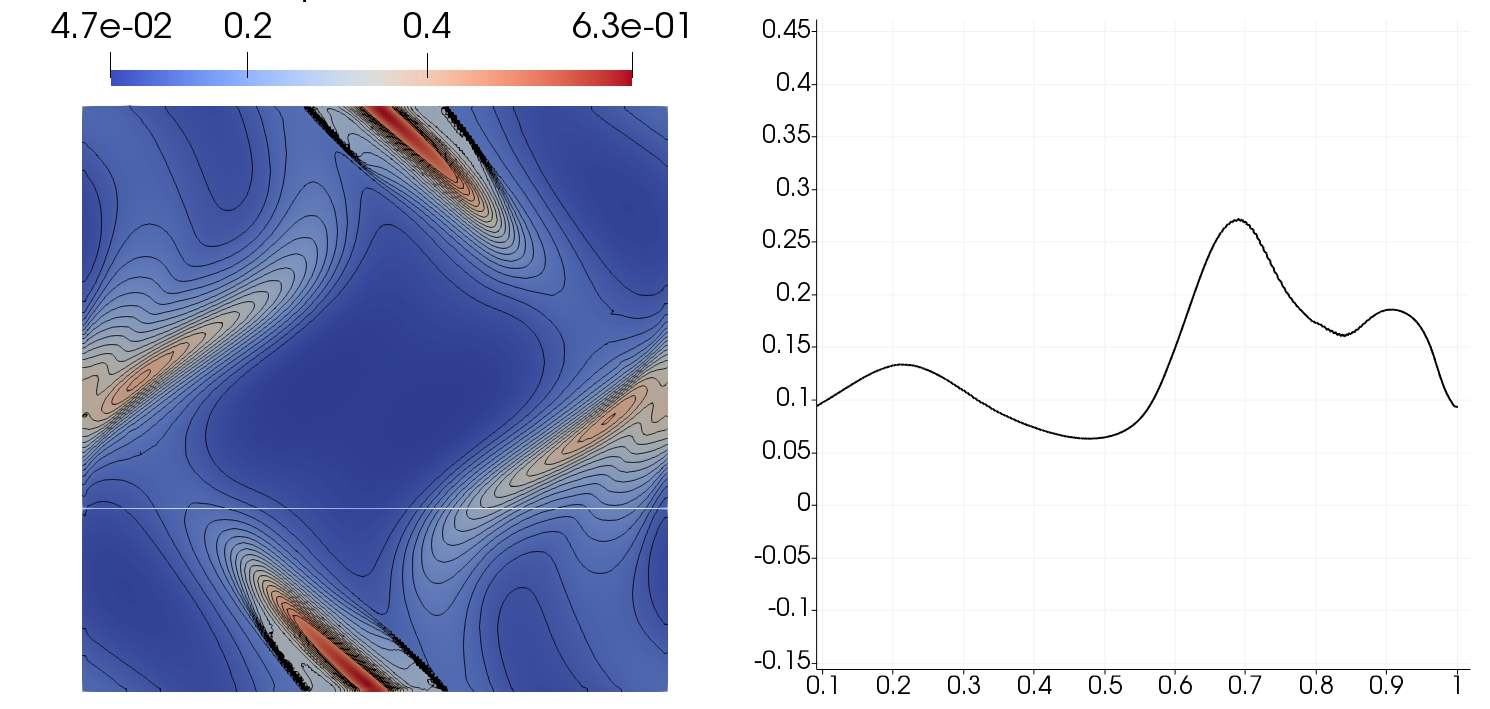
\includegraphics[width=0.92\textwidth]{img/ot/my2new.jpg}
\vspace{-2mm}
\caption{$p$ distribution in $\Omega$ and $p$ along $y = 0.3125$, $t = 0.18$}
\label{figure:myOt2}
\end{figure}
\vspace{-4mm}

\begin{figure}[H]
	\centering
	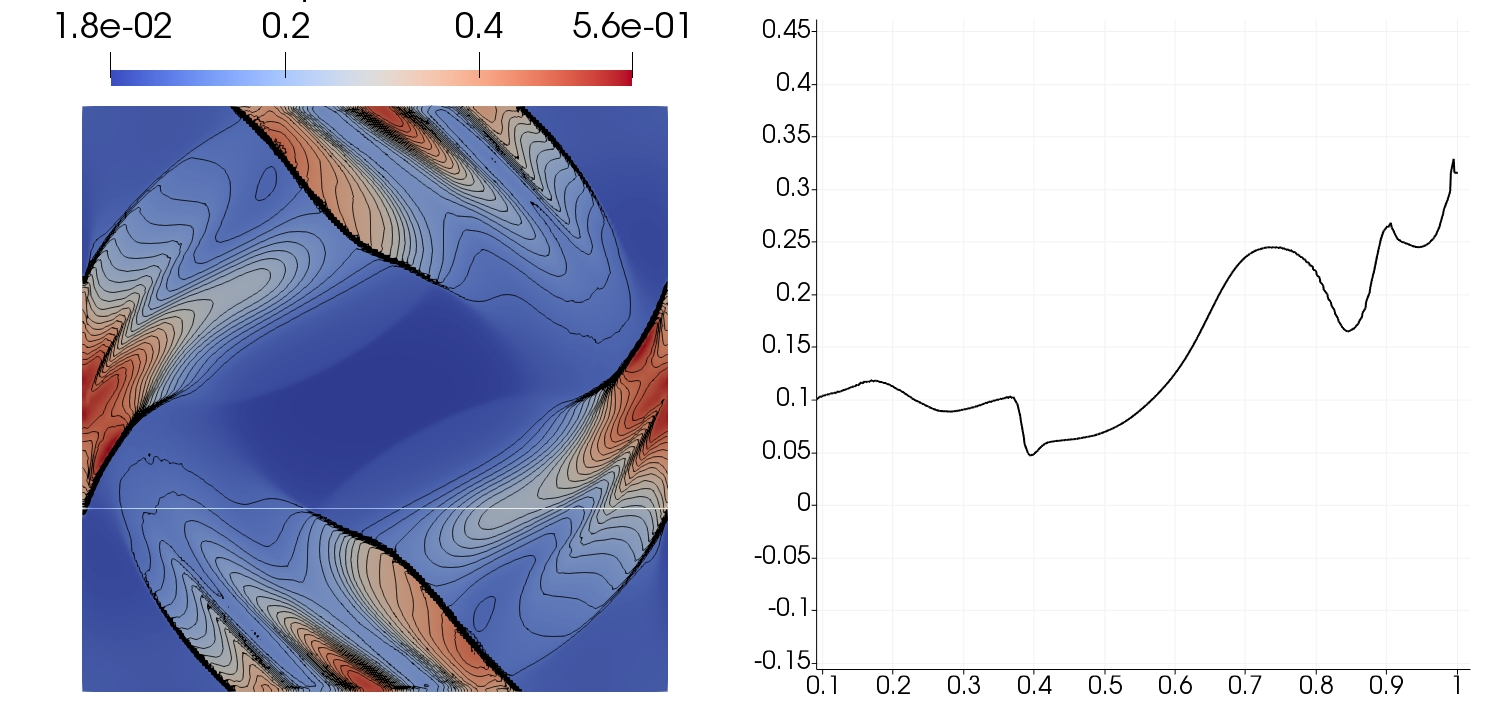
\includegraphics[width=0.92\textwidth]{img/ot/my3new.jpg}
\vspace{-2mm}
\caption{$p$ distribution in $\Omega$ and $p$ along $y = 0.3125$, $t = 0.28$}
\label{figure:myOt3}
\end{figure}
\vspace{-4mm}

\begin{figure}[H]
	\centering
	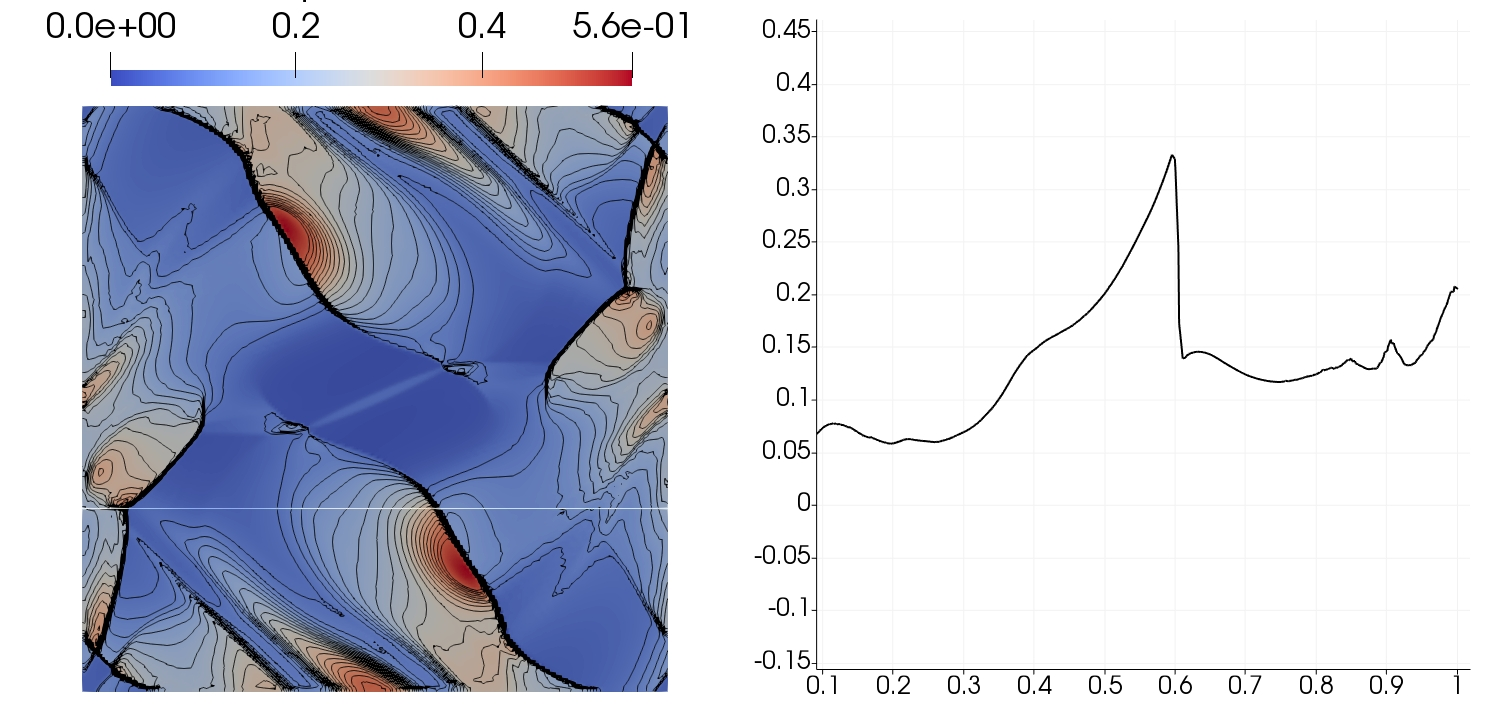
\includegraphics[width=0.92\textwidth]{img/ot/my4new.jpg}
\vspace{-2mm}
\caption{$p$ distribution in $\Omega$ and $p$ along $y = 0.3125$, $t = 0.38$}
\label{figure:myOt4}
\end{figure}
\vspace{-4mm}

\begin{figure}[H]
	\centering
	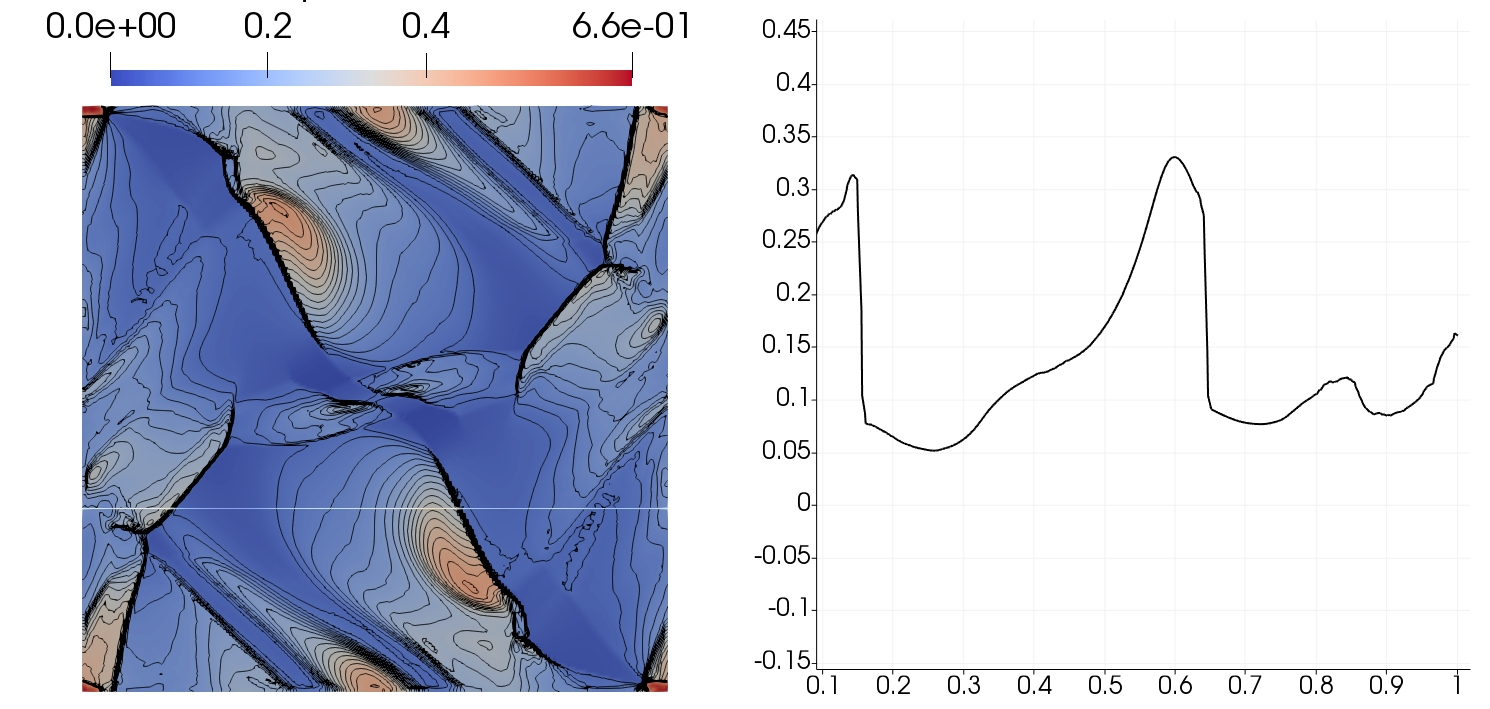
\includegraphics[width=0.92\textwidth]{img/ot/my5new.jpg}
\vspace{-2mm}
\caption{$p$ distribution in $\Omega$ and $p$ along $y = 0.3125$, $t = 0.46$}
\label{figure:myOt5}
\end{figure}
\vspace{-4mm}

\begin{figure}[H]
	\centering
	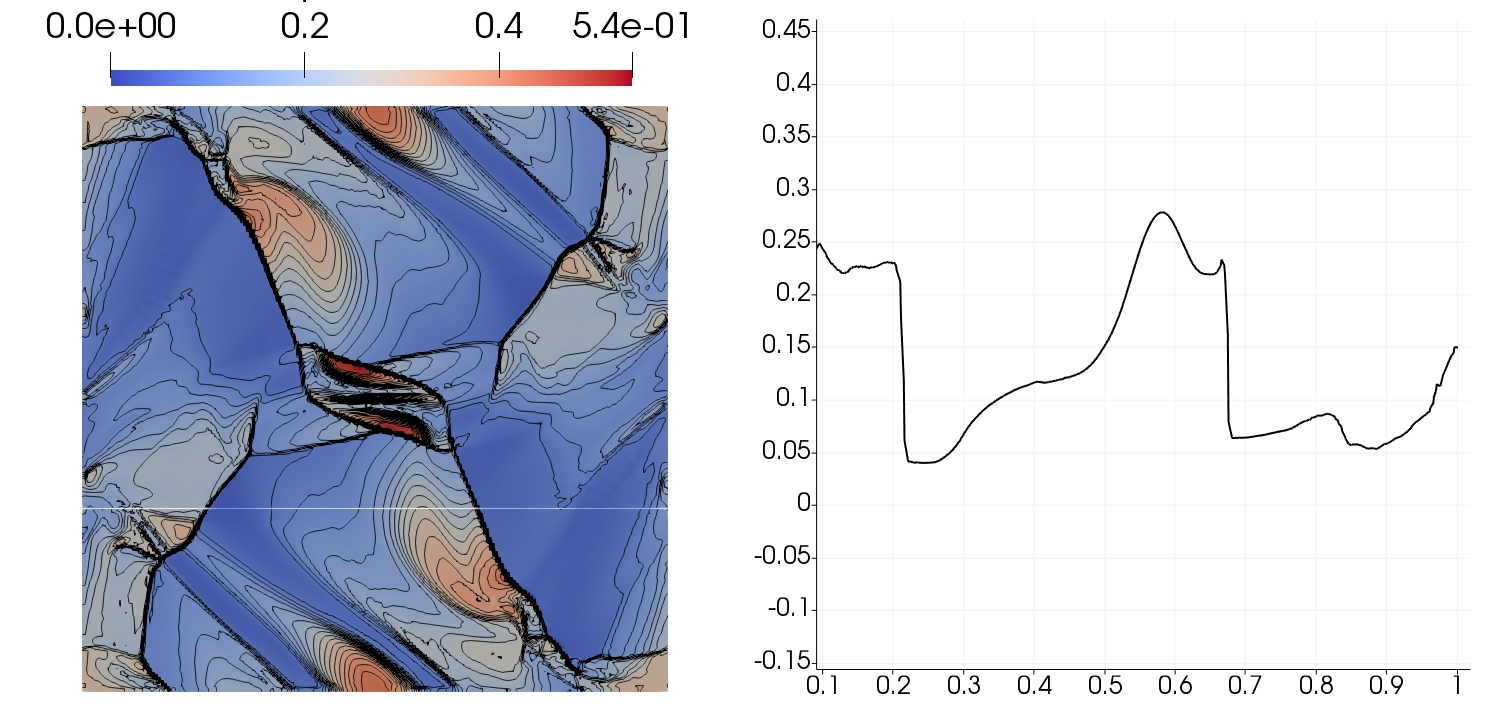
\includegraphics[width=0.92\textwidth]{img/ot/my6new.jpg}
\vspace{-2mm}
\caption{$p$ distribution in $\Omega$ and $p$ along $y = 0.3125$, $t = 0.48$}
\label{figure:myOt6}
\end{figure}
\vspace{-4mm}

\begin{figure}[H]
	\centering
	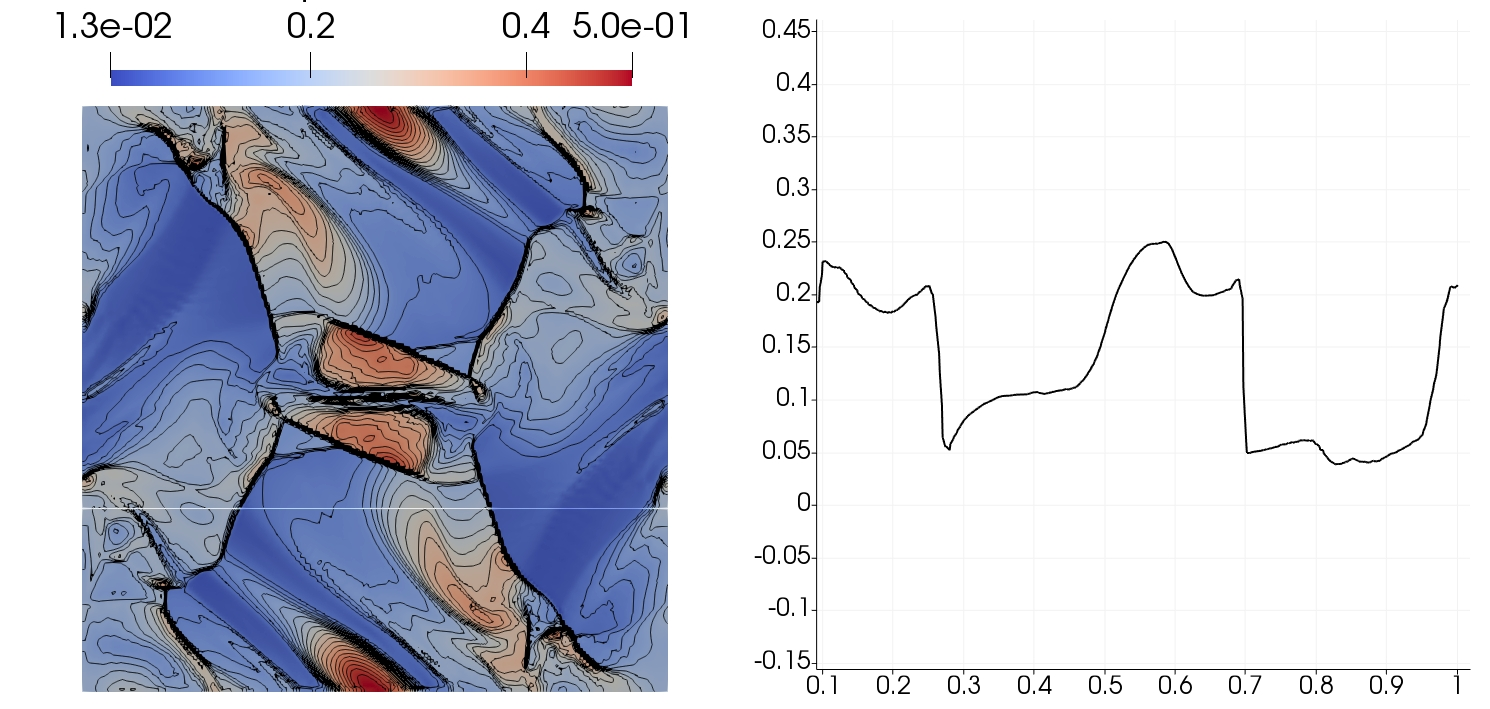
\includegraphics[width=0.92\textwidth]{img/ot/my7new.jpg}
\caption{$p$ distribution in $\Omega$ and $p$ along $y = 0.3125$, $t = 0.5$}
\label{figure:myOt7}
\end{figure}

As noted above these figures, the resolution of all present shocks and discontinuities is very high, and is accordance with the reference results (\cref{figure:otRef}) in \cite{blast1}, and \cite{blast0}.

\section{Flux tube eruption model}
This model is based on the original Titov-Demoulin model from \cite{td}, as used in \cite{miraClanek}, where the geometrical proportions, and equilibrium conditions are taken from \cite{td}.
\subsection{Problem parameters}
The model parameters are as follows. Note that $k_B$ is the Boltzmann constant $k_B = 1.38064852 \times 10^{-23} \frac{\mathrm{J}}{\mathrm{K}}$, $m_p$ is the plasma mass, and $g$ gravitational acceleration. Parameter values read
\begin{align}
\nonumber \beta & =  0.05\ \ \ \ ...\ \text{Plasma beta},\\
\nonumber L_G & =  2\ k_B \frac{T_{ext}}{\lo m_p g \ro} = 1.2 \times 10^8 \left[\text{m}\right],\\
\nonumber L_G & =  20 \ \ \ \ ...\ \text{Coronal height scale in dimension-less units},\\
\nonumber N_t & = 5\ \ \ \ ...\ \text{Torus winding number},\\
\nonumber R & = 3\ \ \ \ ...\ \text{Torus major radius},\\
\nonumber L & = 1.5\ \ \ \ ...\ \text{Magnetic charge separation distance},\\
\nonumber d & =  1.5\ \ \ \ ...\ \text{Geometrical factor},\\
\nonumber q & =  \frac{\ln\lo 8 e^{-5/4} R\ro}{4} N_t \lo\frac{L}{R}\ro^2\left[1 + \lo\frac{R}{L}\ro^2\right]^{3/2},\\
\nonumber q & \approx \text{Normalised magnetic charge corresponding to global equilibrium},\\
\nonumber H & = 2\ \frac{N_t^2}{R^2}\ \ \ \ ...\ \text{"Helicity" factor inside tho loop},\\
\nonumber \frac{ T_{ext} }{T_{in}} & =  10\ \ \ \ ...\ \text{Coronal/prominence temperature ratio}.\\
\end{align}
The domain $\Omega$ is taken as $\left[-2.5, 2.5\right] \times \left[-5, 5\right] \times \left[0, 5\right]$.
\subsection{Initial condition}
The model is equipped with an initial condition:
\begin{align}
\rho\lo\bfx, t_0\ro & = \mathrm{exp}\lo\frac{-z}{\frac{ T_{ext} }{T_{in}}L_G}\ro,\ \bfx\ \text{inside the torus}\\
\rho\lo\bfx, t_0\ro & = \frac{ T_{in} }{T_{ext}} \mathrm{exp}\lo\frac{-z}{L_G}\ro,\ \bfx\ \text{outside the torus}\\
p\lo\bfx, t_0\ro & = \beta\ \text{everywhere}\\
\bfv\lo\bfx, t_0\ro & = 0\ \text{everywhere}\\
\bfB\lo\bfx, t_0\ro & \bfB_{in}\lo\bfx, t_0\ro + \bfB_{ext}\lo\bfx, t_0\ro,
\end{align}
where $t_0 = 0$, and the equations for the magnetic field of the flux rope $\bfB_{in}\lo\bfx, t_0\ro$, magnetic field created by the (artificial) magnetic charges $\bfB_{ext}\lo\bfx, t_0\ro$ are the same as in equations (3) and (4) in \cite{miraClanek}.
\subsection{Boundary conditions}
The model of equilibrium is equipped with these boundary conditions for density $\rho$, pressure $p$, and velocity $\bfv$:
\begin{align}
\frac{\partial \rho}{\partial \bfn} & = 0\ \text{everywhere},\\
\frac{\partial p}{\partial \bfn} & = 0\ \text{everywhere},\\
\frac{\partial \bfv}{\partial \bfn} & = 0\ \text{on the left, right, front, back, and top boundary},\ z > 0,\\
\bfv & = 0\ \text{on the bottom boundary},\ z = 0,\\
\end{align}
where the last equations represents the fixed ends of the flux rope on Sun's surface.
The conditions for the magnetic field are more difficult to set, as we need to make sure that $\nabla \cdot \bfB = 0$ also for the magnetic field across the boundary.
One way to achieve this is to set:
\begin{align}
\frac{\partial B_{t_{1,2}}}{\partial \bfn} & = 0,\\
\frac{\partial B_n}{\partial \bfn} & = -\sum_{i = 1, 2}\frac{\partial B_{t_{i}}}{\partial \bft_{i}},
\end{align}
where $\bfn$ is the normal direction, $\bft_{i}, i = 1, 2$ are the two tangential directions, and $B_n$, and $B_{t_{1,2}}$ stands for the normal, and two tangential components of the magnetic field $\bfB$. Also, $U$ is calculated from the above so that the relation \cref{presU} holds.

